\label{Chapter6}
\chapter{Results}
\lhead{Chapter 6. \emph{Results}}
%=======================================================
\section{Computation of resonant frequencies and modes}
%text
\label{sc:FrequenciesAndModes}
%=======================================================

The proposed strategy to compute the resonant frequencies and associated modes in a cavity consist on two stages described in this section. 

%=======================================================
\subsection{Resonant frequencies}
%text
\label{sc:frequencies}
The computation of the resonant frequencies of a cavity using a time domain solver is performed by integrating in time the Maxwell's equations using an initial condition or current source designed to excite the frequencies within a desired interval $[f_m, f_M]$. The use of localised pulses designed to excite a broad range of frequencies is commonly used~\cite{guo2001computation,taflove2013advances,dantanarayana2014resonant} although it is possible to exclude unwanted frequencies by carefully exciting the fields~\cite{werner2008extracting}.

The solution is then advanced using a time marching algorithm and the electromagnetic fields are recorded at one or several points. In this work we employ an explicit fourth order Runge-Kutta scheme for advancing the solution in time. When combined with the spatial DG discretisation described in the previous section, this results in an efficient and low-storage approach because the resulting mass matrix is block diagonal~\cite{HybridMeshesCEM}. 

At the end of the time domain simulation, a signal processing algorithm is applied to the recorded fields in order to compute the resonant frequencies. The most popular choice is the fast Fourier transform (FFT) but other alternatives such as the filter diagonalisation method (FDM~\cite{FDM}) are able to provide the same accuracy as FFT with shorter signals (i.e, shorter runs of the time domain solver). Figure~\ref{fig:comparisonFFT_FDM} shows a comparison of the error on a computed resonant frequency as a function of the final time of the time domain simulation using FFT and FDM. 
%figure DONE FDM (maybe remove)
\begin{figure}[!ht]
	\centering
	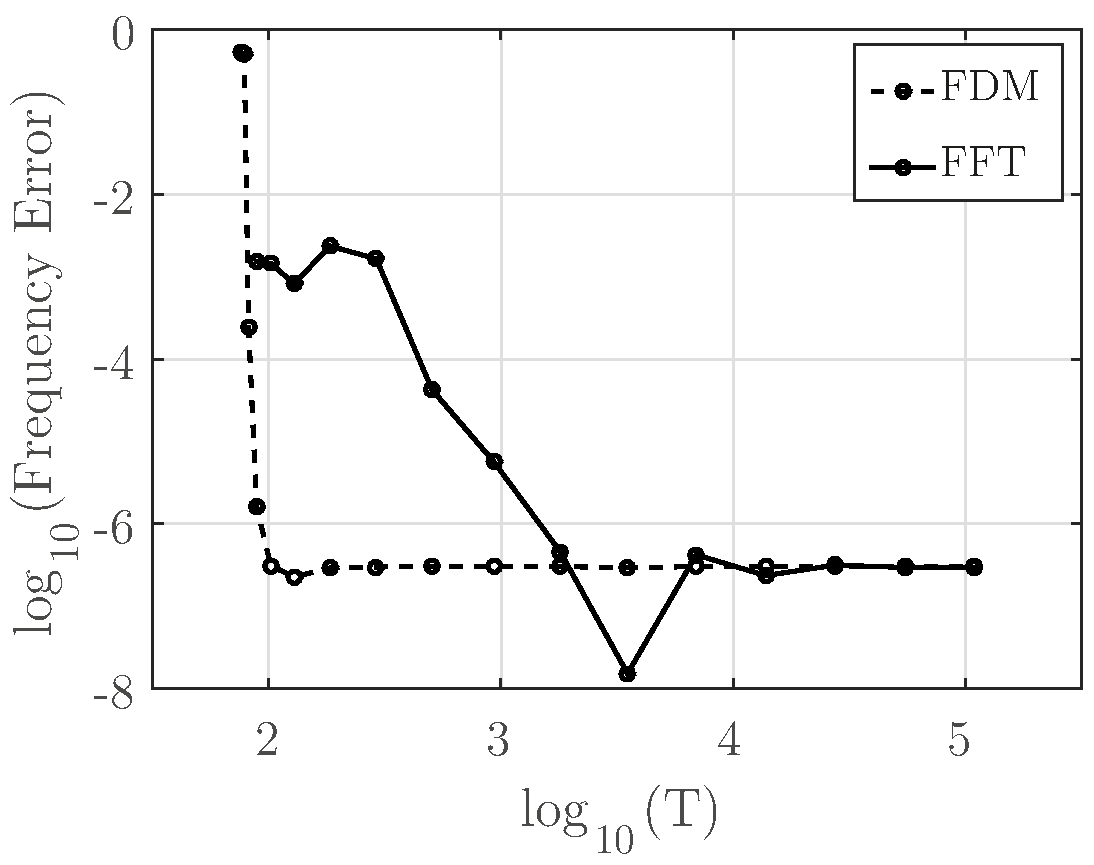
\includegraphics[width=0.6\textwidth]{figs/comparisonFFT_FDM}
	\caption{Error on a computed resonant frequency as a function of the length of the signal for FFT and FDM.}
	\label{fig:comparisonFFT_FDM}
\end{figure}
%TODO specify the units of time (T) somewhere in the text for an example
%geometry (so that I know what order they are for a problem of interest)
%text
It can be clearly observed that FDM is able to provide the same accuracy than FFT by reducing the final simulation time by more than two orders of magnitude. A detailed comparison of different frequency extraction techniques has been recently presented in~\cite{dantanarayana2014resonant}.

The choice of the monitor/s points can have an important effect on the final spectrum obtained. For instance, if a monitor point coincides (or it is very close) to a symmetry point of a particular mode, the frequency associated to this mode will not be obtained when applying the signal processing algorithm to the recorded signal. This effect has been studied in detail in~\cite{stark2009positional} and also can be utilised to avoid exciting undesired modes. 

Finally, it is worth mentioning that filters are commonly applied to the recorded fields to reduce the spectral leakage effect induced by the length of the signal~\cite{harris1978use,madisetti2009digital}. For the examples considered in this work the FDM is applied to the recorded signals and a Blackman filter is applied before extracting the frequency content. 

%=========================================================

\subsection{Resonant modes}
%text
\label{sc:modes}
After the resonant frequencies are computed, the associated resonant modes are computed by performing a second run of the time domain solver with a built-in discrete Fourier transform, namely
\begin{equation*}
    \hat{\USoltn}_j(f_k) = \sum_{n=0}^{\nT-1} \USoltn_j (t_n) \exp(-i2\pi t_n f_k), \quad j=1,\cdots,\nnode,
\end{equation*}
where $\nT$ is the total number of time steps, $\Delta t$ is the time step, $i = \sqrt{-1}$, $f_k$ are the computed resonant frequencies,  $t_n = n\Delta t$ and $\nnode$ is the total number of mesh nodes.


%=======================================================

\section{Numerical examples} 
%text
\label{sc:examples}

This sections presents a number of numerical examples to validate the implementation of the proposed technique for both free-space and dispersive materials. A comparison of the performance of low and high-order elements is presented and the effect of the geometric representation of cavities with curved boundaries on the accuracy and convergence properties of the proposed methodology are presented.

%============================================================

\subsection{Rectangular free space cavity}
%text
\label{sbc:freeSpace2D}

The first example involves the computation of the resonant frequencies and associated modes on a rectangular metallic cavity of dimension $2L \times L$ where $L=$20$\mu$m filled with air. The objective is to show the optimal convergence of the proposed approach for approximating the resonant frequencies and compare the performance of high and low-order approximations.  

The TM mode is considered and the frequencies are computed using a series of
structured quadrilateral meshes with 4$\times$2, 8$\times$4, 16$\times$8,
32$\times$16 and 64$\times$32 elements and different degrees of approximation.
The spectra obtained is shown in Figure~\ref{fig:rectangle2DfreeSpace_Spectrum}
\begin{itemize}
\item EXAMPLE INTRODUCTION (PHYSICS)
\item show the analytical solution
\item refer to a reference problem (i.e. length etc)
\item show a table of first 10 analytical solution values (up to $f=2$) with $f_1...f_10$ labels
\item include the analytical frequencies for the reference problem in the table
\item EXAMPLE INTRODUCTION (NUMERICS)
\item say the type of initial condition (delta, location, intensity)
\item final time + timesteps used (for each example) : make sure everything is
  normalised (same final time)
\item say that the way the initial condition is represented depends on the shape functions.
\item say that spectrum computed is the UNION of all the components (justify by
  saying that this shows all frequencies that have been captured).
\end{itemize}

note: TM only has one "good" component (which is U3), and TE has two U1 and U2 (but no U3) is the only component 
%figure
\begin{figure}[!ht]
	\centering
  \subfigure[4$\times$2 ]{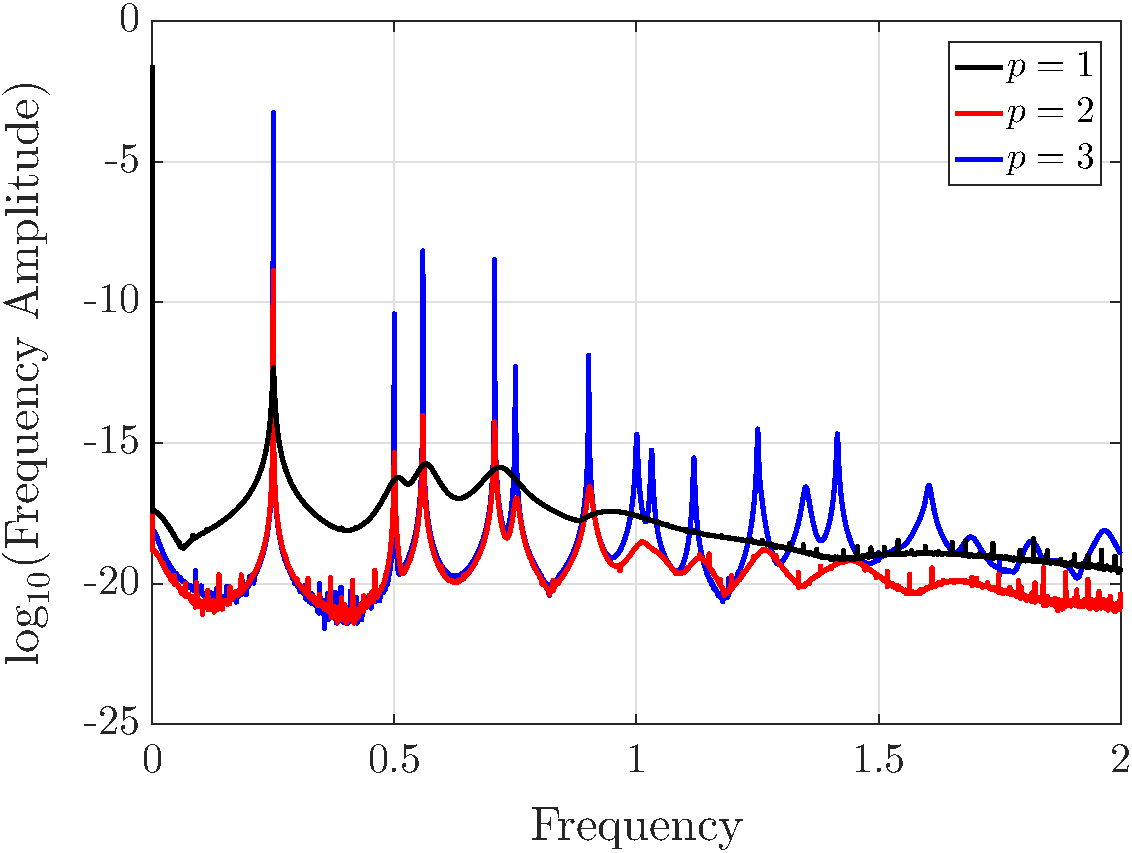
\includegraphics[width=0.49\textwidth]{2D_FreeSpaceCavity/spectra/spectrum2x4}}
  \subfigure[16$\times$8 ]{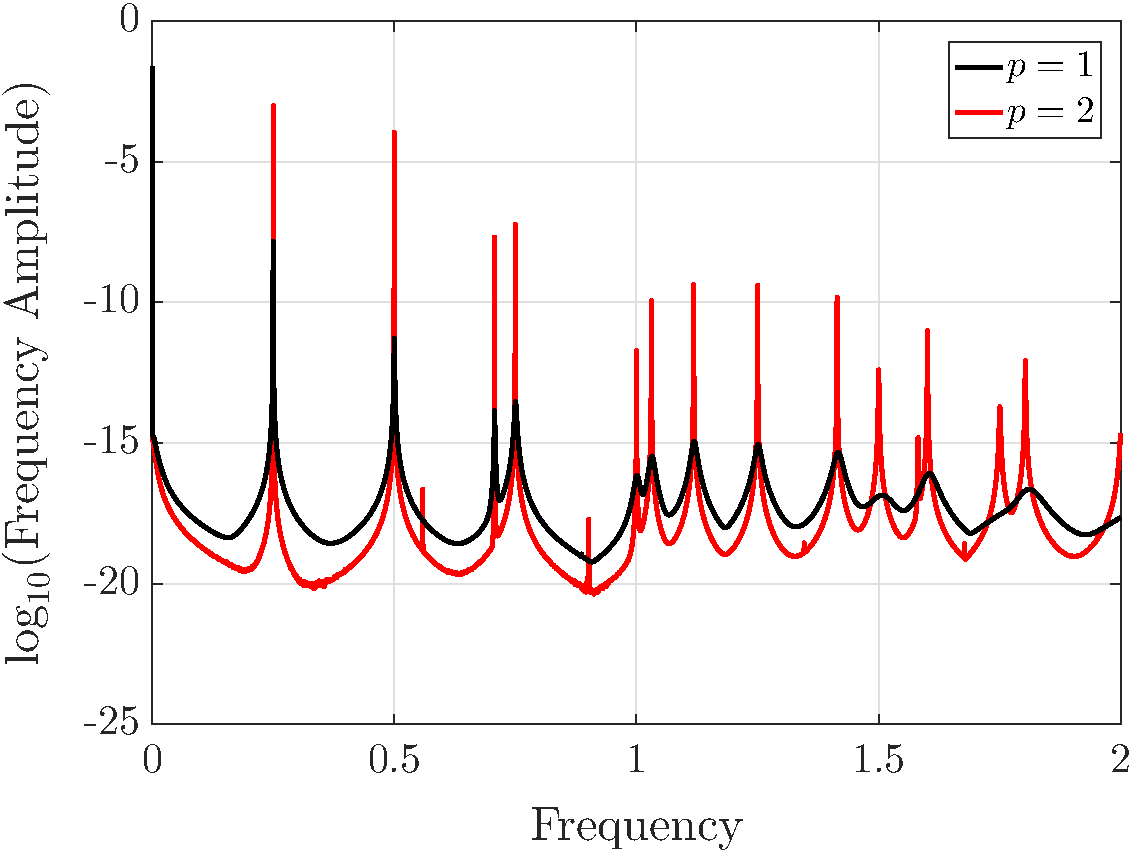
\includegraphics[width=0.49\textwidth]{2D_FreeSpaceCavity/spectra/spectrum8x16}}
	\caption{Rectangular free space cavity: spectra for two meshes of quadrilaterals for different $p$.}
	\label{fig:}
\end{figure}
TODO: double check that the same point IC and the same final time is used in each case.
TODO: change the spectra to be LENGTHWAYS (maybe less tall?) - check font size
not affected

\begin{itemize}
\item PLOT 1
\item discuss the advantages of high order (higher frequency + higher amplitude)
\item say WHY we want higher amplitude...maybe this should have already happened by this stage?
\item all frequencies captured up to...
\item some comments about peak at zero
\item PLOT 2
\item Focus on the lowest frequency, compare the p=1 fine mesh vs p=2 coarse
  mesh, p=2 fne vs p=3 coarse (give ndof, nsteps for each example, total cpu time numbers)
\item discuss the initial condition, we are using a delta function, which means
\item mention that some frequencies are not captured
\item mention that this is due to initial condition, and could be modified by: gaussian, multiple initial conditions
\item show a plot of p=2, 16x8 with multiple initial conditions
\item need to mention peak WIDTH (for the same final time?), make sure the final
  time is ACTUALLY the same - width should be a measure of quality factor
\item mention that these are done using a Blackman envelope (haven't introduced
  this yet!!)
\end{itemize}

Figure~\ref{fig:rectangle2DfreeSpace_Convergence} shows the evolution of the error on four computed resonant frequencies as a function of the element size for a degree of approximation $p$ ranging from 1 up to 3.
%figure
TODO: cut out the points (p2 8x16) has some time marching error!
TODO: Add extra (higher error) points to make plots more asthetically pleasing
TODO: Add legends to all figures
\begin{figure}[!ht]
	\centering

   \subfigure[$f_{1} \approx, \USoltn_{2}, \TEz $]{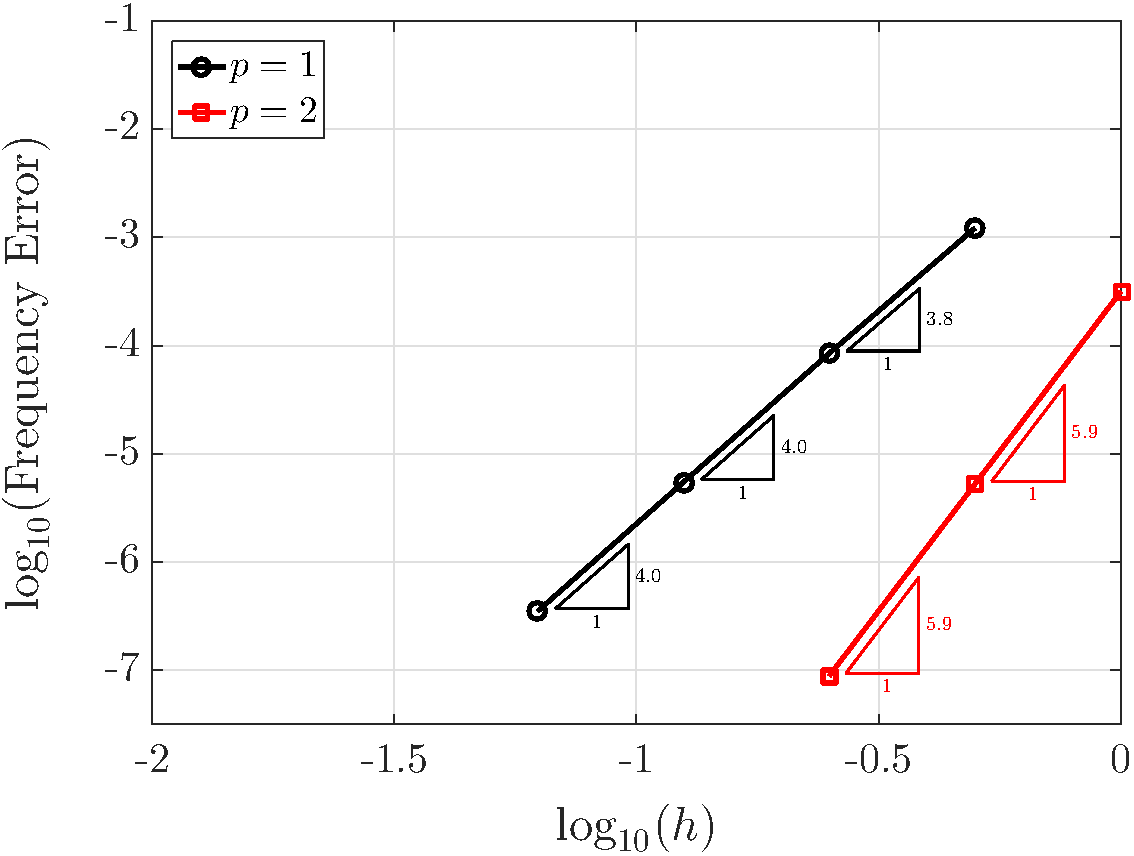
\includegraphics[width=0.49\textwidth]{2D_FreeSpaceCavity/Conv/U[2]/F1_TE}}
   \subfigure[$f_{2} \approx, \USoltn_{1}, \TEz $]{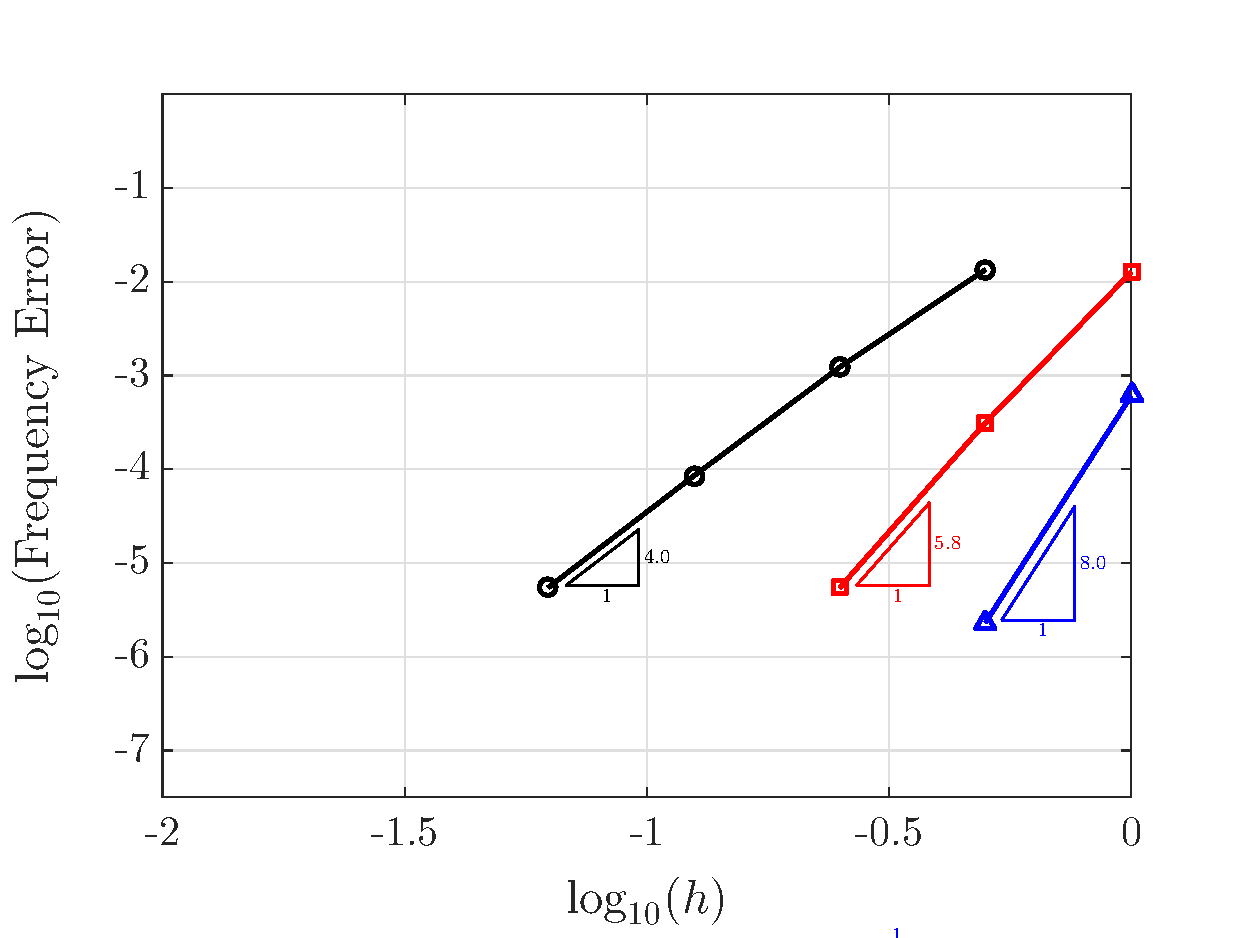
\includegraphics[width=0.49\textwidth]{2D_FreeSpaceCavity/Conv/U[1]/F2_TE}}
   \subfigure[$f_{3} \approx, \USoltn_{3}, \TMz $]{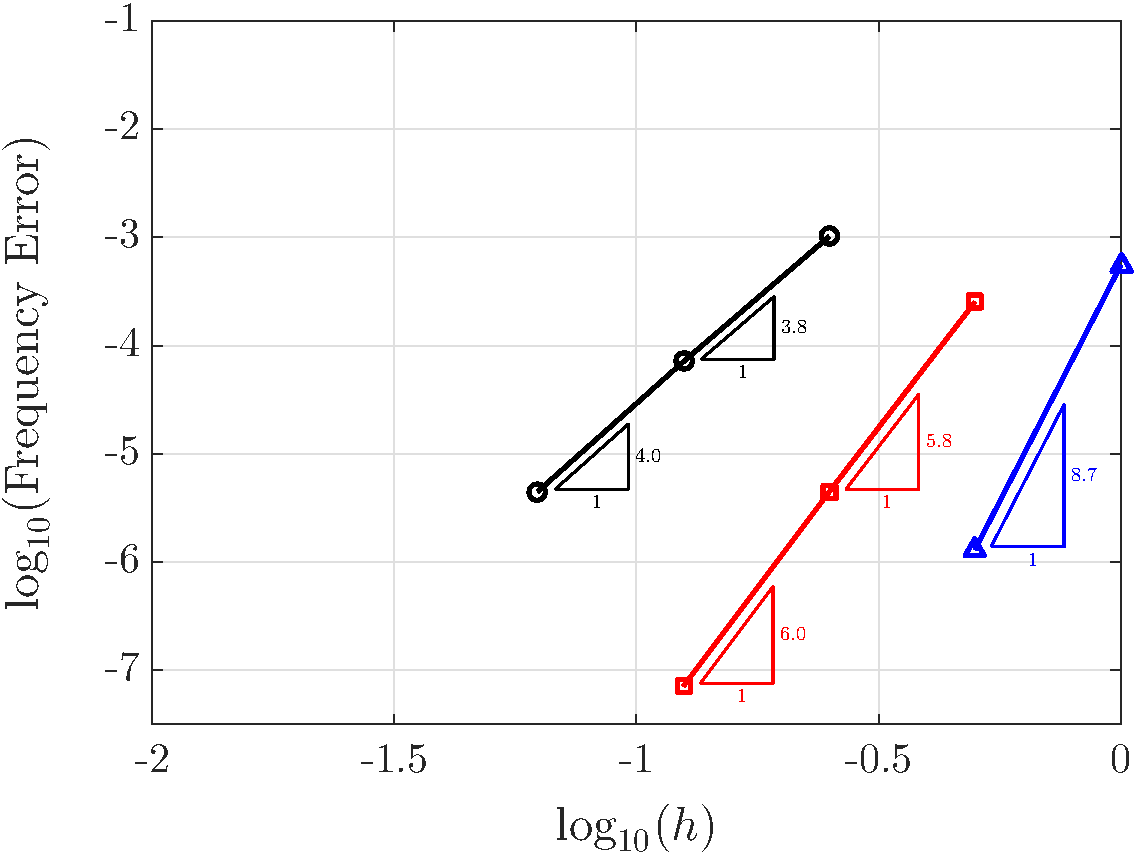
\includegraphics[width=0.49\textwidth]{2D_FreeSpaceCavity/Conv/U[3]/F3_TM}}
   \subfigure[$f_{6} \approx, \USoltn_{2}, \TMz $]{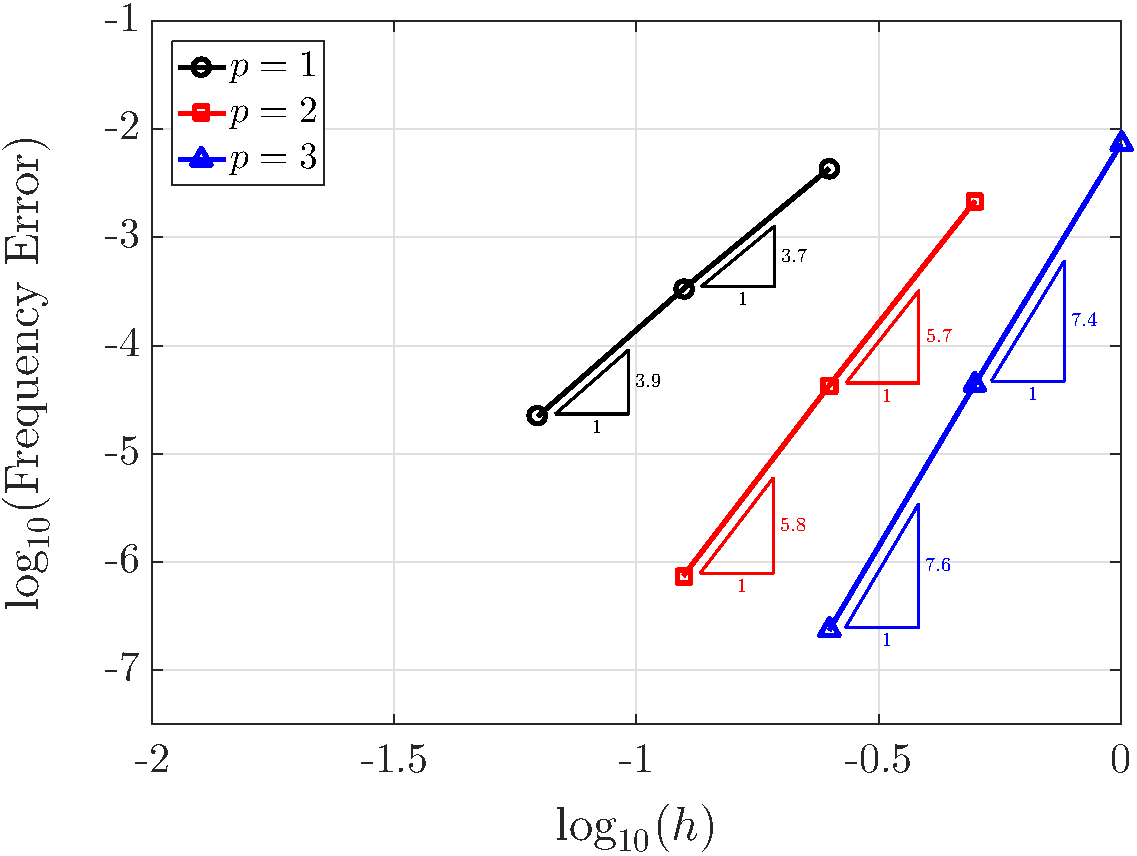
\includegraphics[width=0.49\textwidth]{2D_FreeSpaceCavity/Conv/U[2]/F6_TM}}
   \subfigure[$f_{8} \approx, \USoltn_{3}, \TMz $]{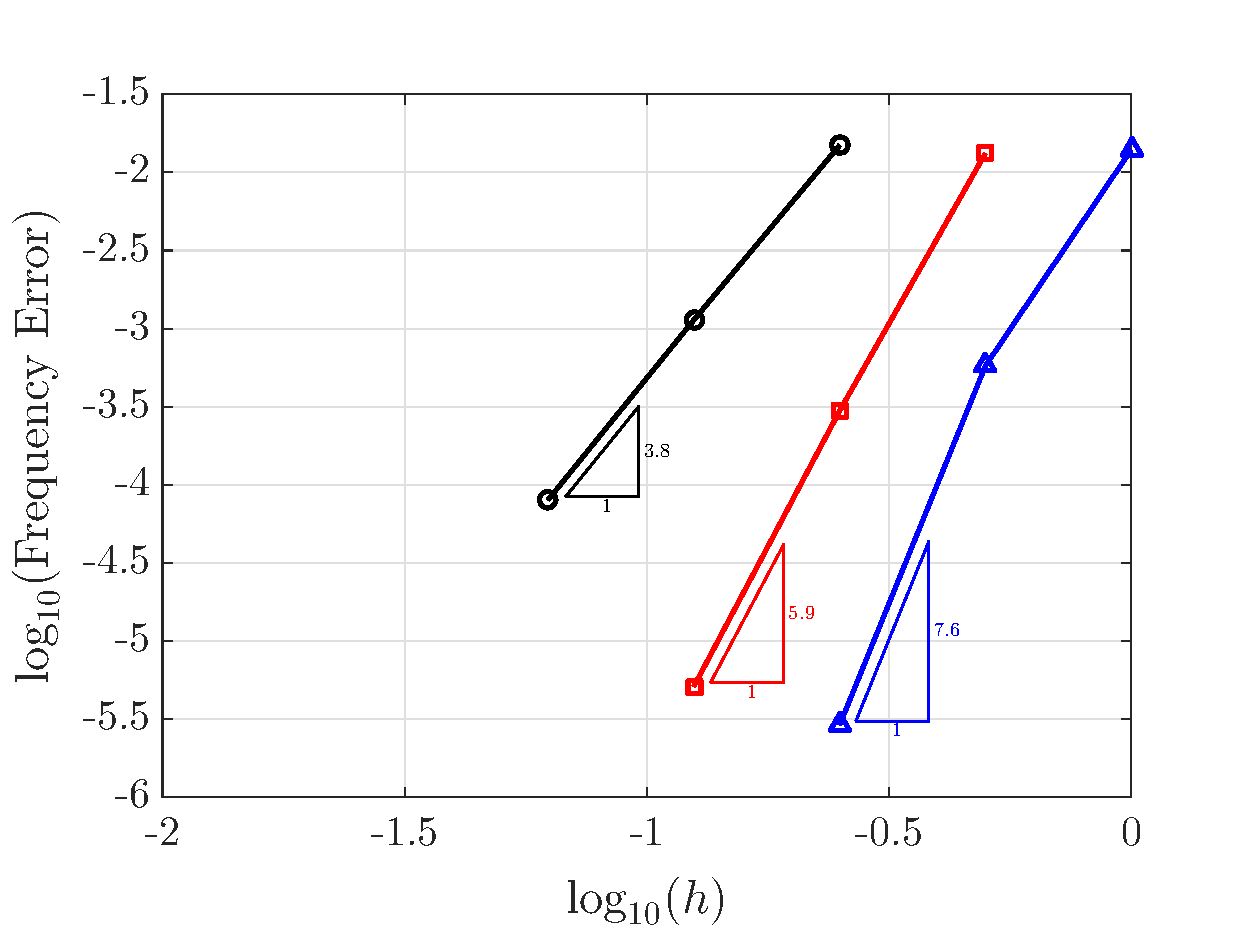
\includegraphics[width=0.49\textwidth]{2D_FreeSpaceCavity/Conv/U[3]/F8_TM}}
   \subfigure[$f_{10} \approx, \USoltn_{3}, \TMz $]{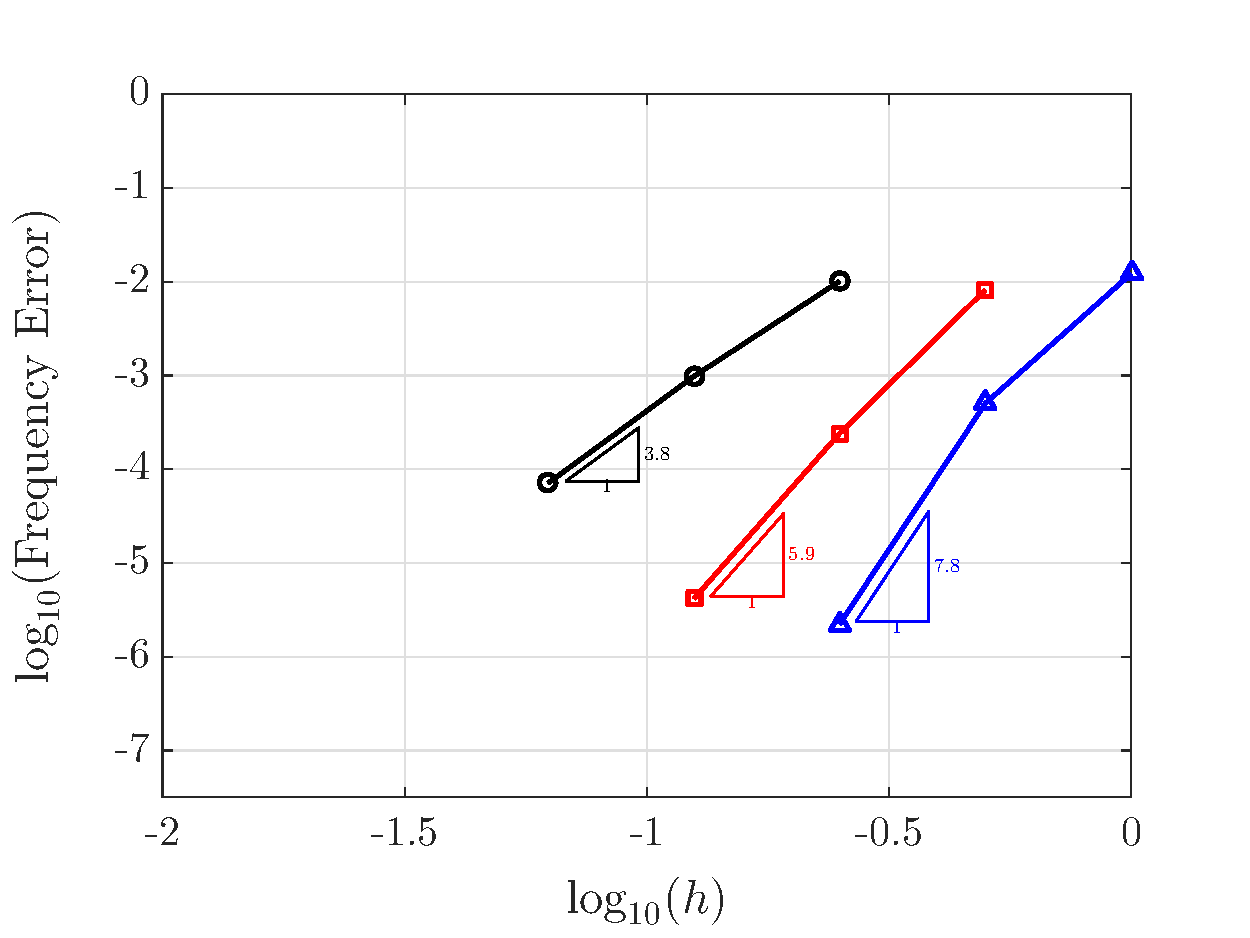
\includegraphics[width=0.49\textwidth]{2D_FreeSpaceCavity/Conv/U[3]/F10_TM}}
	\caption{Rectangular free-space cavity: $h$-convergence of the error for six resonant frequencies.}
	\label{fig:rectangle2DfreeSpace_Convergence}
\end{figure}
\begin{itemize}
\item RECTANGULAR CAVITY CONVERGENCE PLOTS
\item *only* a single component has been used, any component could have been used
\item refer to which components/modes used for which plot in the text
\item all components could have been used - this is easier
\item initial condition selected to excite these modes
\item find a reference for the 2p+2 convergence rate
\end{itemize}
%text
In this figure, and in subsequent examples, $f_i$ denotes the computed $i$-th resonant frequency and the frequencies are assumed ordered from lower to higher, i.e. $f_i < f_j$ if $i<j$. The error in the computed frequency $f_i$ is evaluated as $\epsilon_i = (|f_i - f_i^\star|)/f_i^\star$, where $f_i^\star$ is the known exact value of the resonant frequency~\cite{BalanisBook}.

In all the examples, the expected $2p+2$ rate of convergence is approximately obtained, confirming the optimality of the proposed approach for computing the resonant frequencies of a free-space cavity. It can be observed that, for a given mesh and degree of approximation, the error increases as the frequency increases, illustrating the challenge in approximating higher frequencies. For instance, if the third mesh is used with a linear approximation (i.e., $p$=1), the resonant frequency $f_3 \approx$  8.38 THz is computed with an accuracy of $6.1 \times 10^{-4}$ whereas the error on the computed frequency $f_9 \approx$ 16.76 THz is $3.9 \times 10^{-3}$ (i.e. the error on the $f_9$ is more than 6 times higher than the error on the frequency $f_3$).

The results also illustrate the benefit of using high-order approximations. In the second mesh, the use of a cubic approximation of the solution offers a result almost four orders more accurate than using a linear approximation and two orders of magnitude more accurate than using a quadratic approximation. In the four cases presented in Figure~\ref{fig:rectangle2DfreeSpace_Convergence}, the use of a cubic approximation in the second mesh provides a similar accuracy than the computation in the finest mesh with a linear approximation. This implies that the computation with $p$=3 provides the same accuracy than the computation with $p$=1 by reducing the number of degrees of freedom by a factor of almost 20. It is worth mentioning that the required use of finer meshes with linear elements induces a significantly higher computational cost due to the use of an explicit time marching scheme.

After computing the resonant frequencies, the associated modes can be extracted by performing a discrete Fourier transform as described in Section~\ref{sc:FrequenciesAndModes}. Figure~\ref{fig:rectangle2DfreeSpace_modes} shows the second component of the electric field for the four modes associated to the frequencies $f_3$, $f_4$, $f_6$ and $f_9$.
%figure DONE Rectangular cavities
\begin{figure}[!ht]
	\centering
	\subfigure[$f_3 \approx$  8.38 THz]{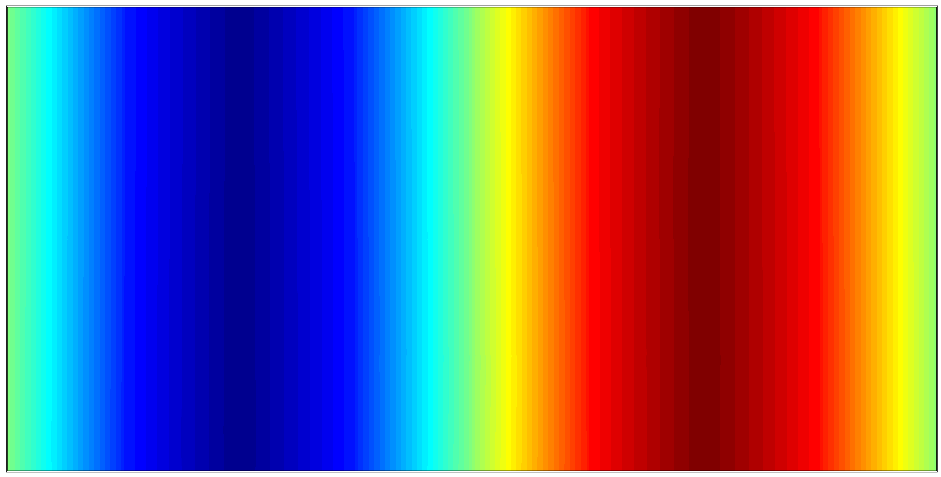
\includegraphics[width=0.24\textwidth]{2D_FreeSpaceCavity/modeShapes/rectangleFreeSpace_U2_Mode2}}
	\subfigure[$f_4 \approx$ 10.60 THz]{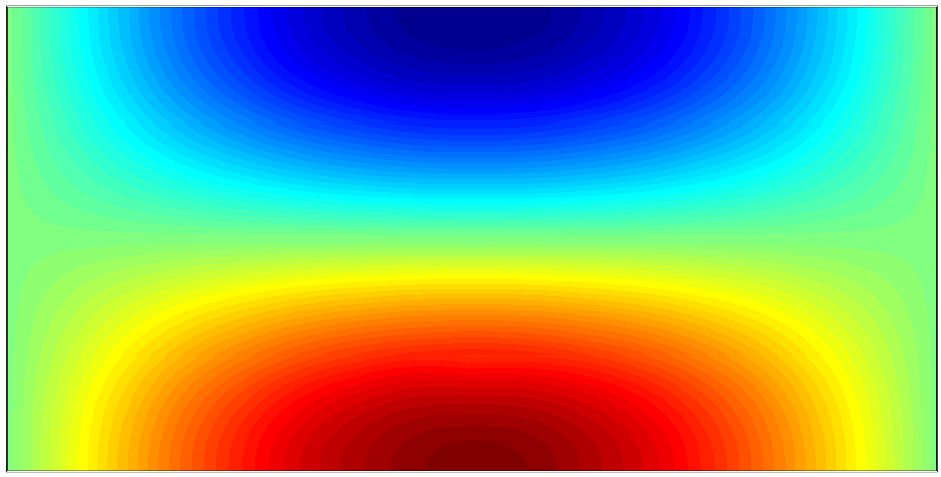
\includegraphics[width=0.24\textwidth]{2D_FreeSpaceCavity/modeShapes/rectangleFreeSpace_U2_Mode3}}
	\subfigure[$f_6 \approx$ 13.51 THz]{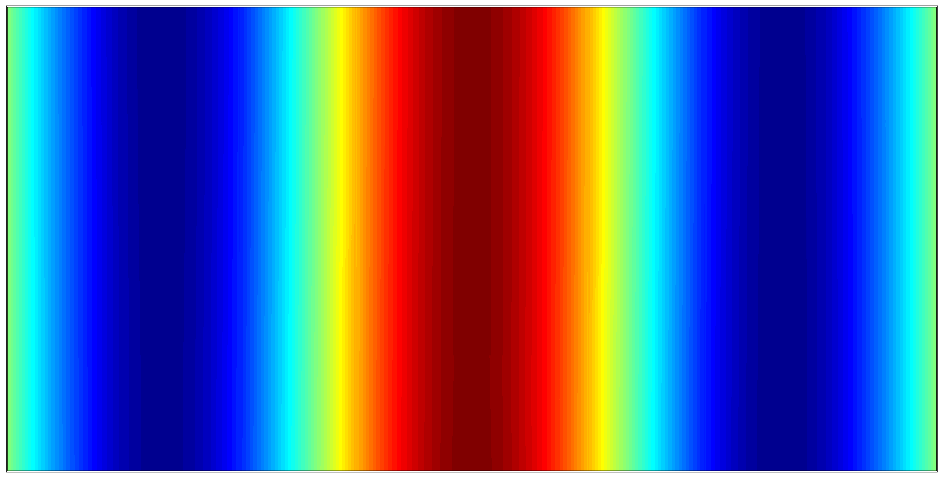
\includegraphics[width=0.24\textwidth]{2D_FreeSpaceCavity/modeShapes/rectangleFreeSpace_U2_Mode5}}
	\subfigure[$f_9 \approx$ 16.76 THz]{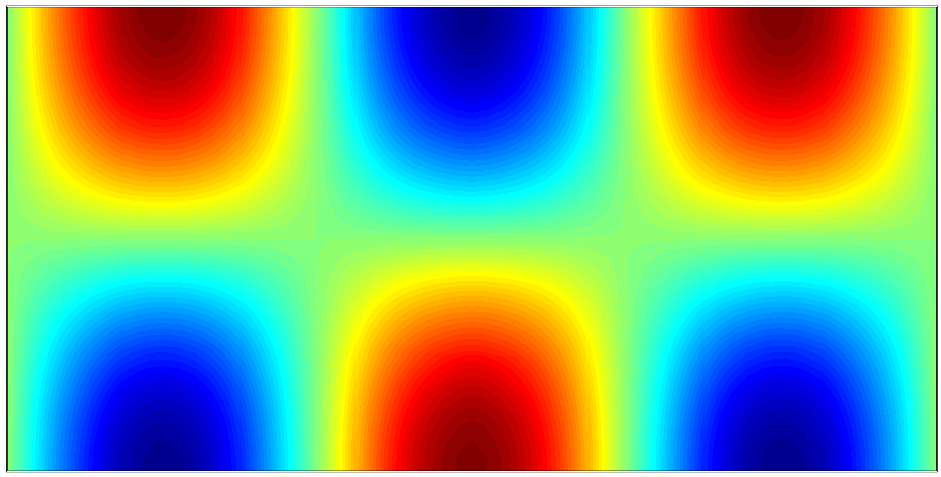
\includegraphics[width=0.24\textwidth]{2D_FreeSpaceCavity/modeShapes/rectangleFreeSpace_U2_Mode6}} 
	\caption{Rectangular free-space cavity: component $E_2$ of four resonant modes.}
	\label{fig:rectangle2DfreeSpace_modes}
\end{figure}

%text
To further illustrate the potential of the proposed approach, Figure~\ref{fig:rectangle2DfreeSpace_modesHF} shows the first electric and magnetic component of the electromagnetic field corresponding to a high frequency mode, with associated resonant frequency of $f_{26} \approx 31.80$ THz. 
%figure DONE high-frequency rectangular cavities
\begin{figure}[!ht]
	\centering
	\subfigure[$E_1$]{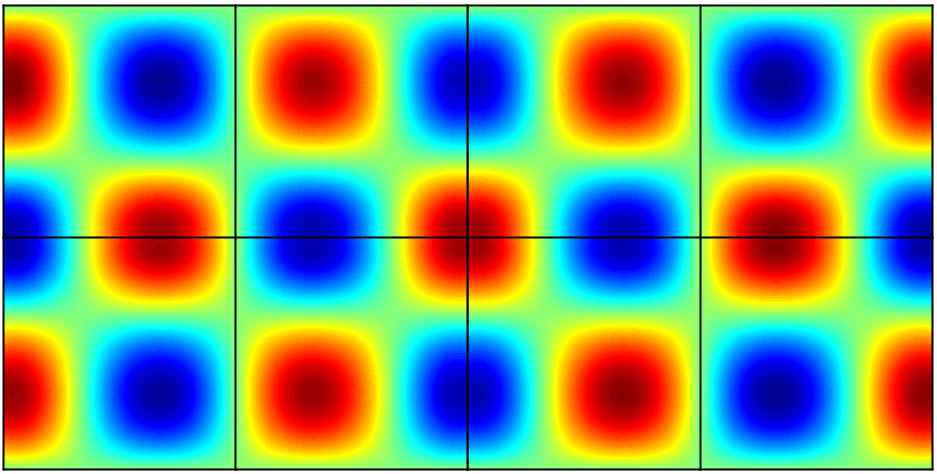
\includegraphics[width=0.45\textwidth]{2D_FreeSpaceCavity/modeShapes/rectangleFreeSpace_2x4_p4_f15_U1}}
	\hspace{1cm}
	\subfigure[$H_1$]{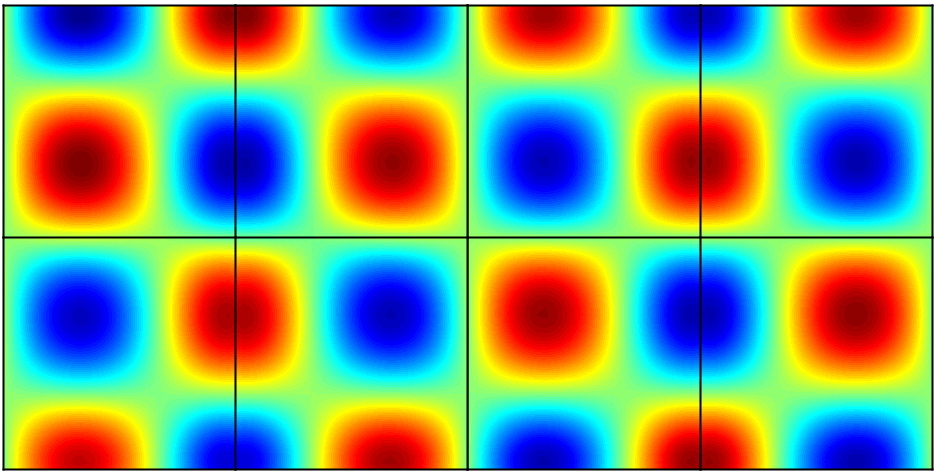
\includegraphics[width=0.45\textwidth]{2D_FreeSpaceCavity/modeShapes/rectangleFreeSpace_2x4_p4_f15_U4}}
	\caption{Rectangular free-space cavity: two components of a high frequency resonant mode corresponding to the resonant frequency $f_{26} \approx 31.80$ THz.}
	\label{fig:rectangle2DfreeSpace_modesHF}
\end{figure}
%text
The computation has been performed on a very coarse mesh with only 8 elements and using a degree of approximation $p$=4 and the high quality of the mode shape can be clearly observed.

%============================================================
%============================================================
\clearpage
\subsection{Aliasing effects}
%figure TODO: make whole width of page to show spectra, use the p=3 mesh above?
\begin{figure}[!ht]
	\centering
\subfigure[$\Delta t = 0.025$]{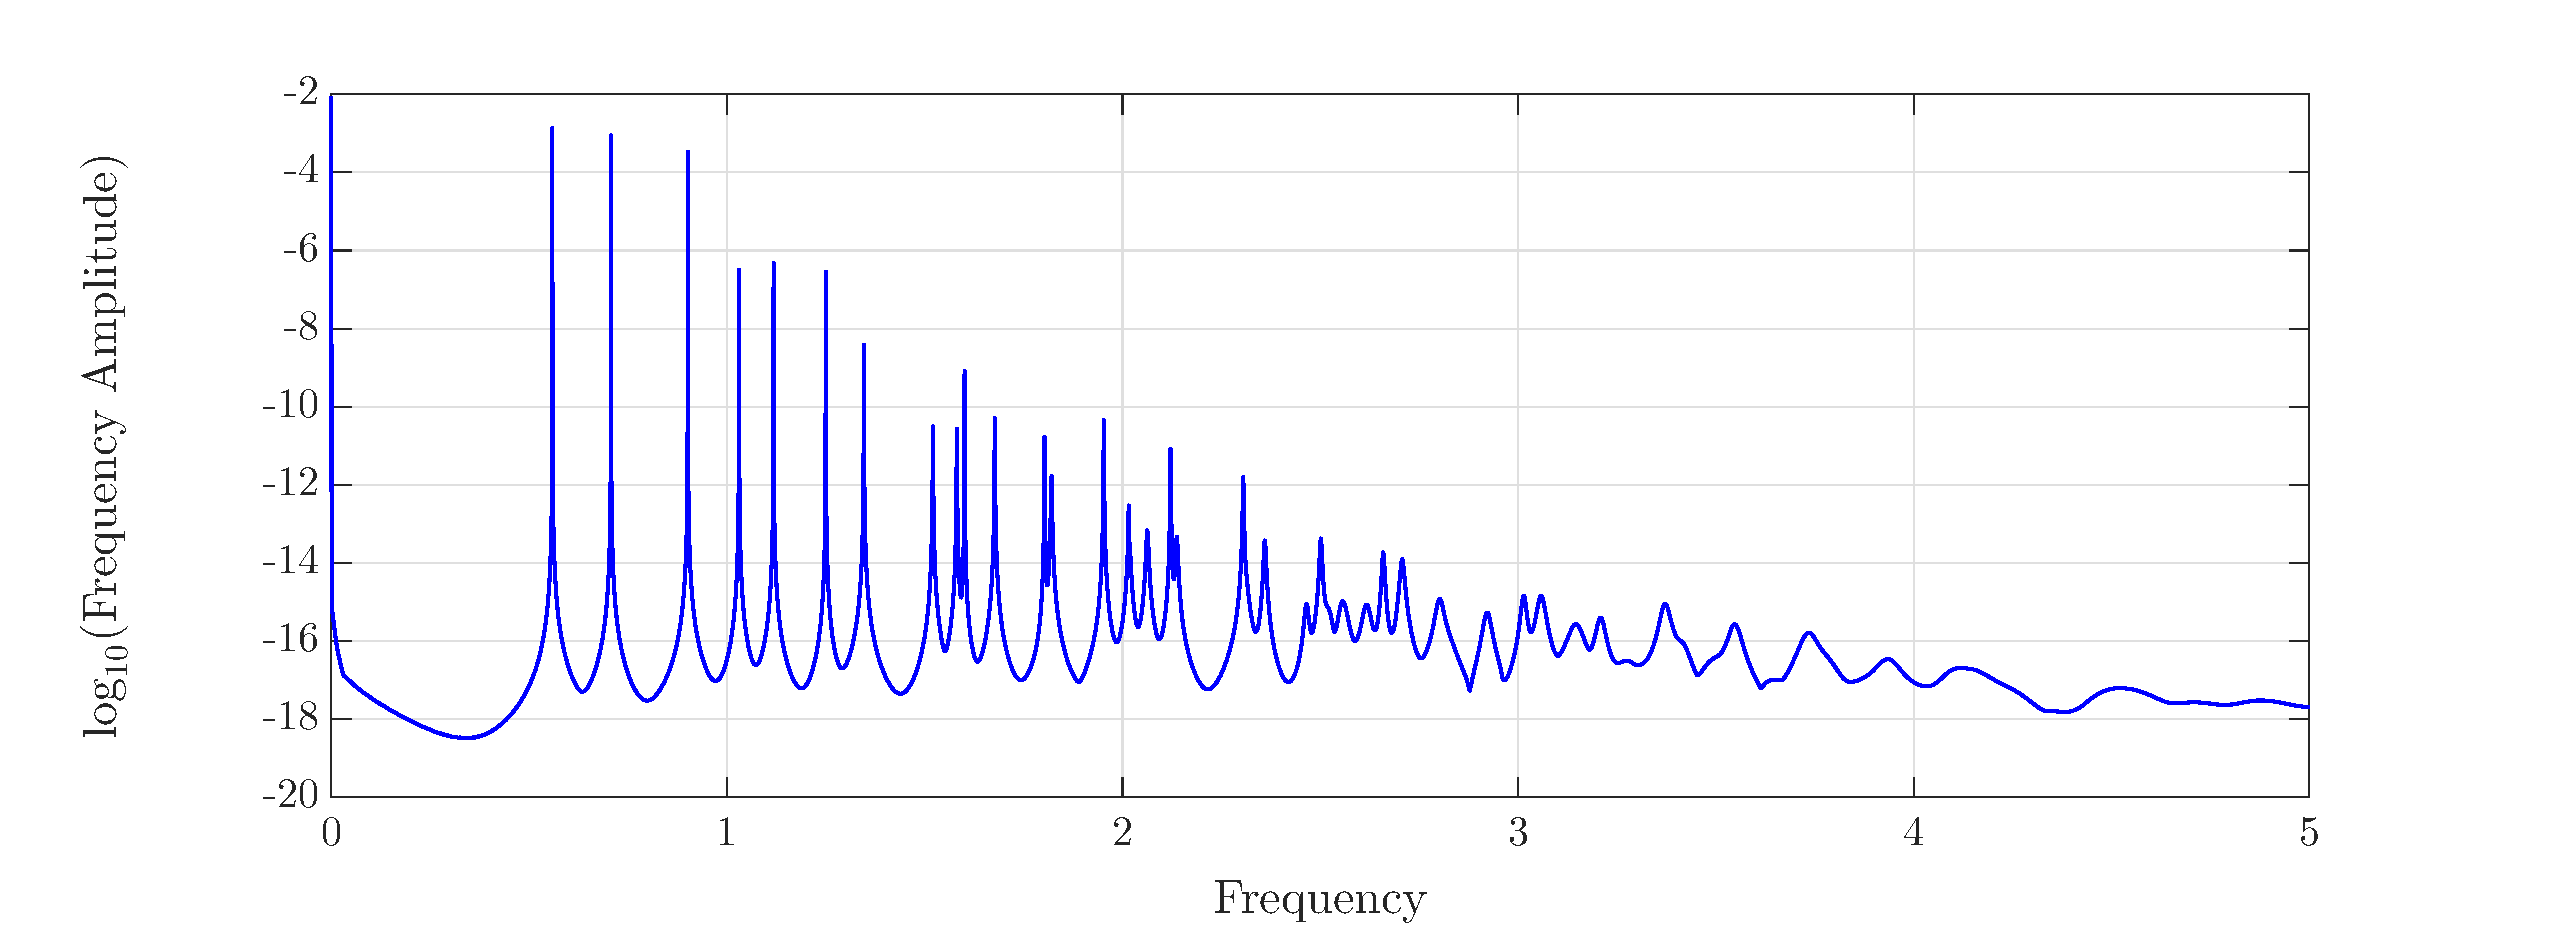
\includegraphics[width=\textwidth]{2D_FreeSpaceCavity/Aliasing/4x8_p3_TM_notaliased}} \\
\subfigure[$\Delta t = 0.2$]{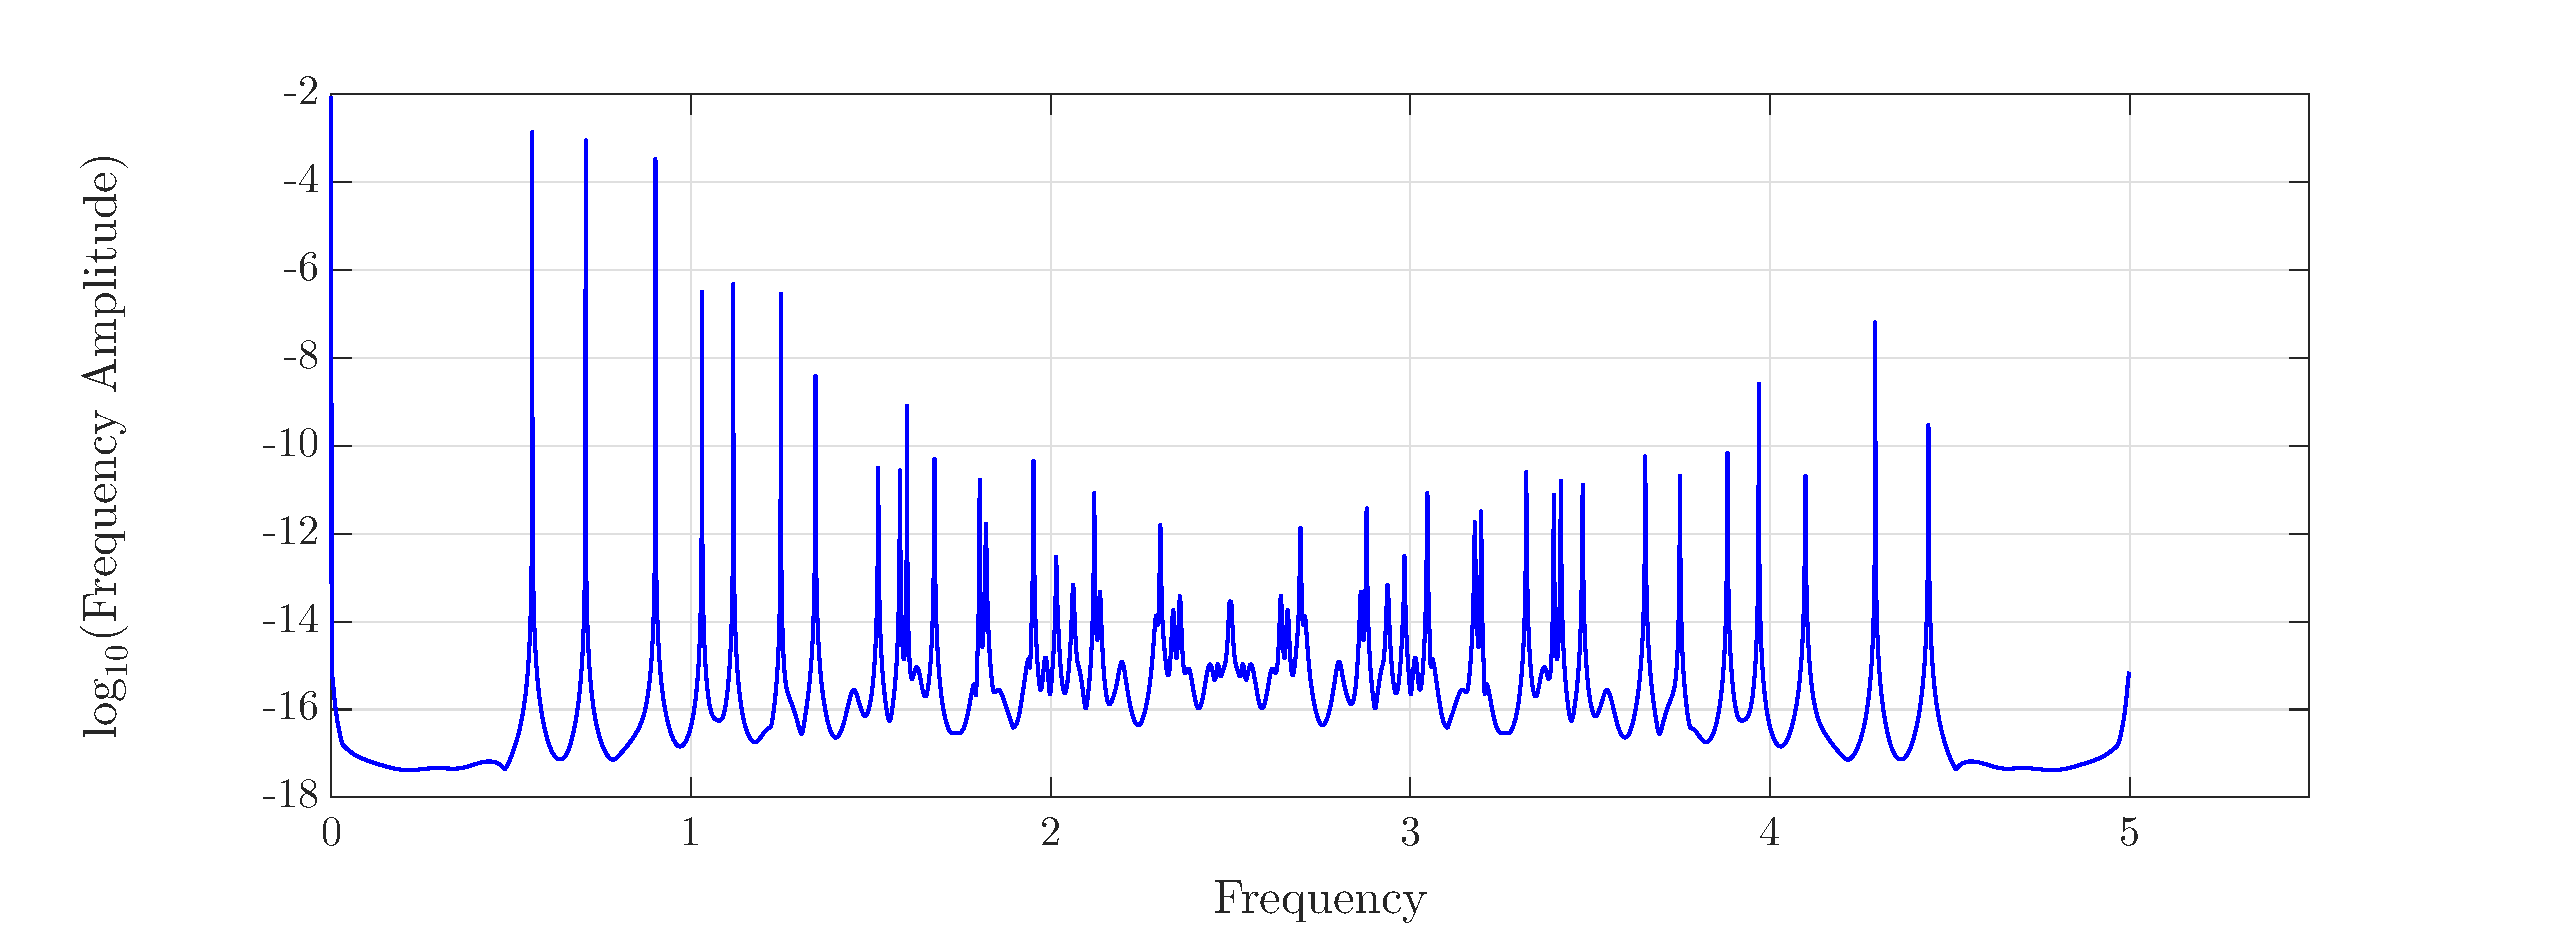
\includegraphics[width=\textwidth]{2D_FreeSpaceCavity/Aliasing/4x8_p3_TM_dt0_2}} \\
\subfigure[$\Delta t = 0.4$]{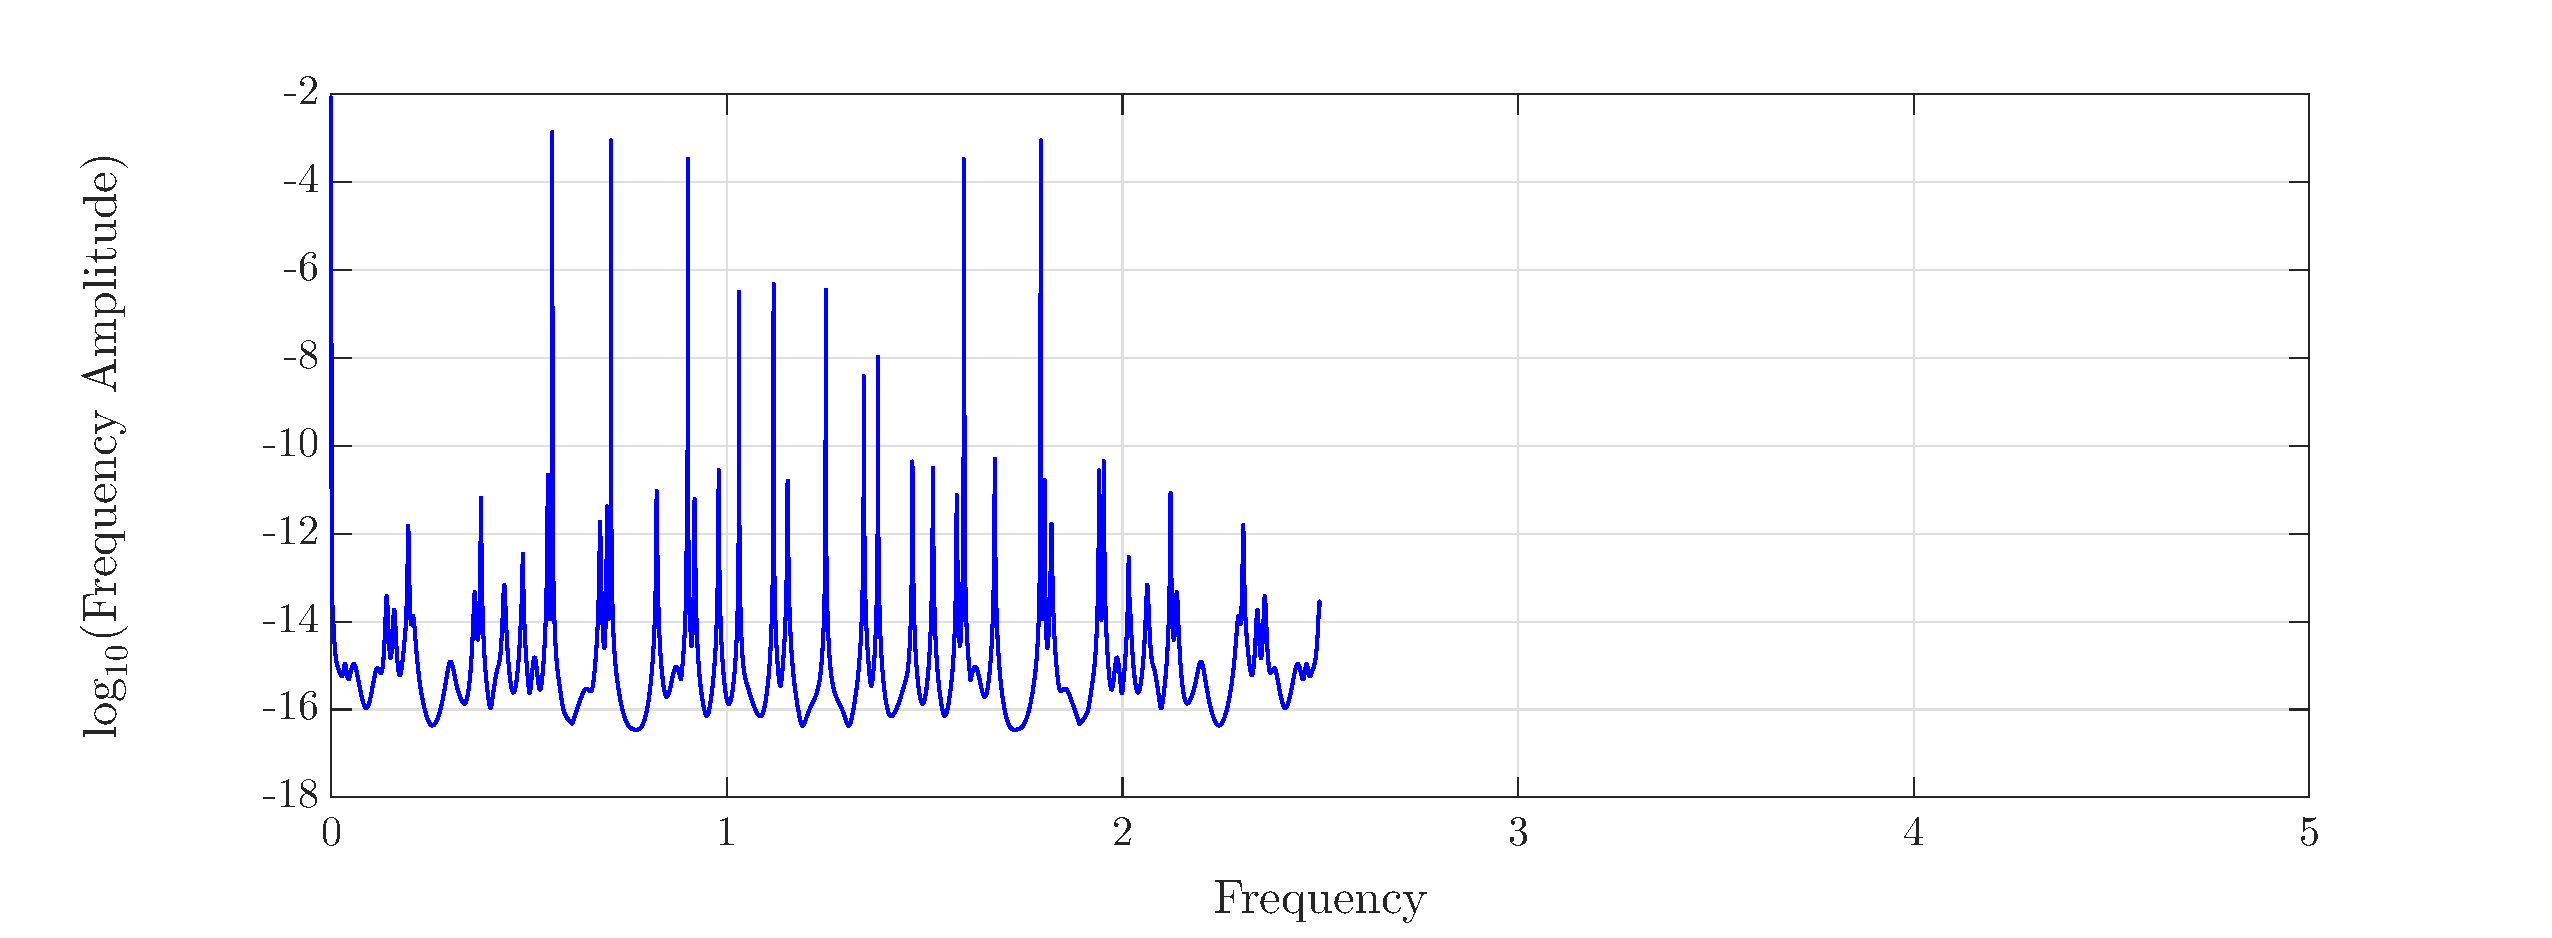
\includegraphics[width=\textwidth]{2D_FreeSpaceCavity/Aliasing/4x8_p3_TM_aliased}} \\
	\caption{Rectangular free-space cavity: spectrum with and without aliasing
    effects for two choices of timestep}
	\label{fig:rectangle2DfreeSpace_modesHF}
\end{figure}

%text TODO
spectrum - $T = 418300$, zero padded to $2^{ 24 }$, $\TMz$ mode, same IC as above
peaks which coincide have a higher amplitude
say in words that the timestep has no effect on error (no need for plot -
doesn't show much)

%figure TODO figure showing modes and convergence (i.e. FEM as a filter)

\clearpage
\subsection{Window functions}
%text TODO
same mesh for both sets of plots:
mesh 16 $\times$ 8 , $p = 2$ and $\TMz$ mode
                x: [-0.5000 0]
             mode: 'TM'
    nOfComponents: 3
     nOfTimeSteps: 896000
               dt: 0.0250
\begin{figure}[!ht]
	\centering
\subfigure[$T=10$]{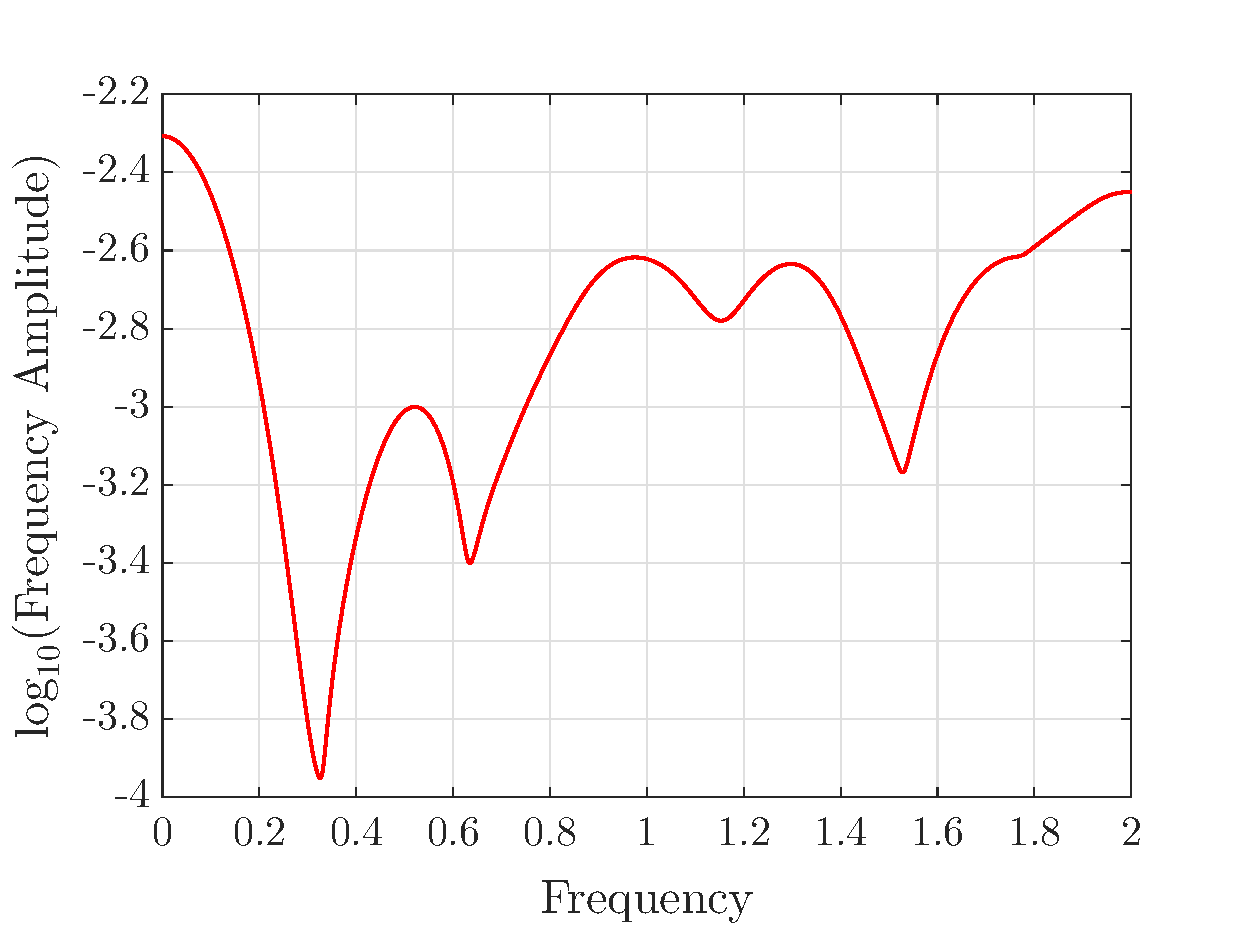
\includegraphics[width=0.49\textwidth]{Windows/spectra/BlackmanHarris-T10}} \subfigure[$T=100$]{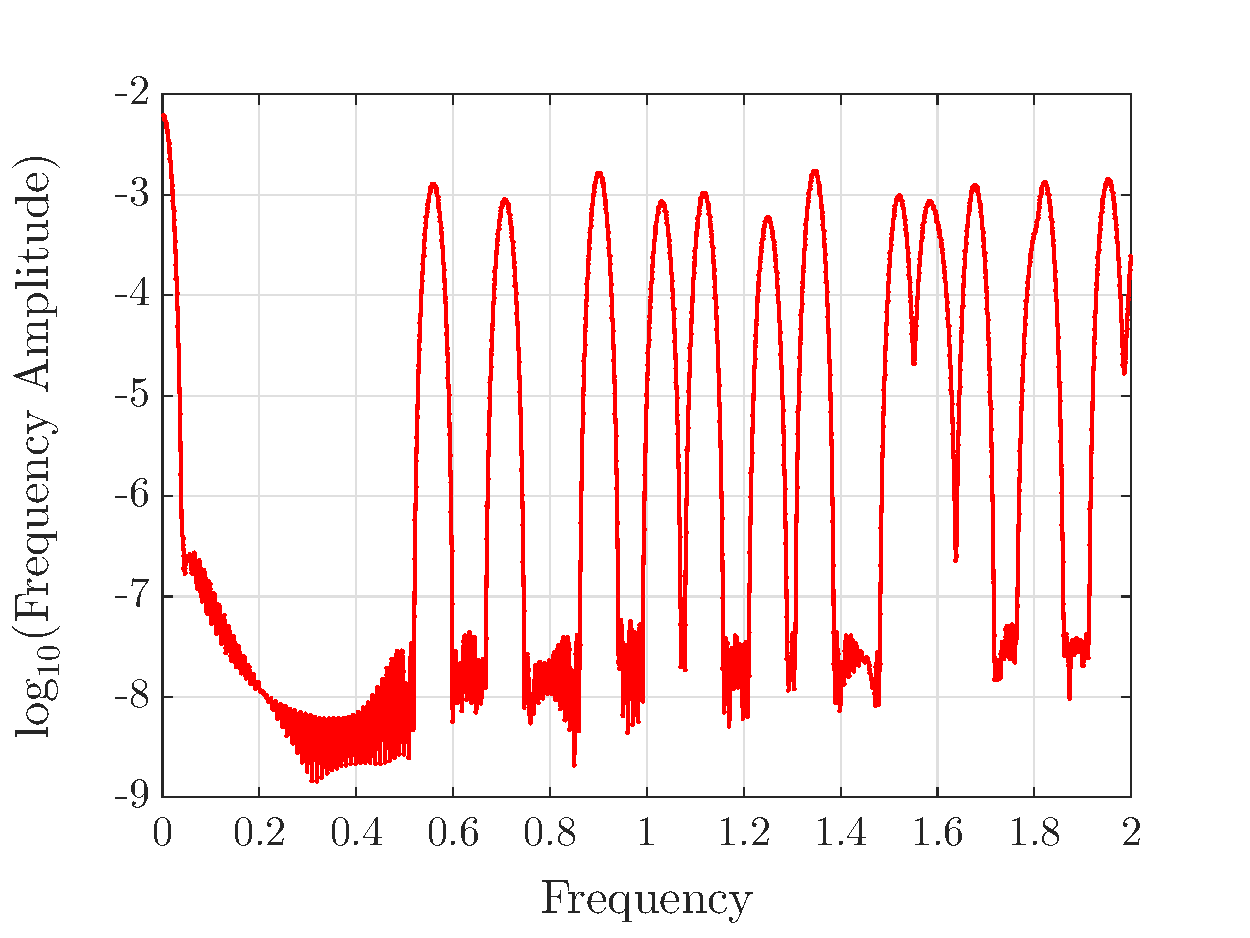
\includegraphics[width=0.49\textwidth]{Windows/spectra/BlackmanHarris-T100}}
\subfigure[$T=1000$]{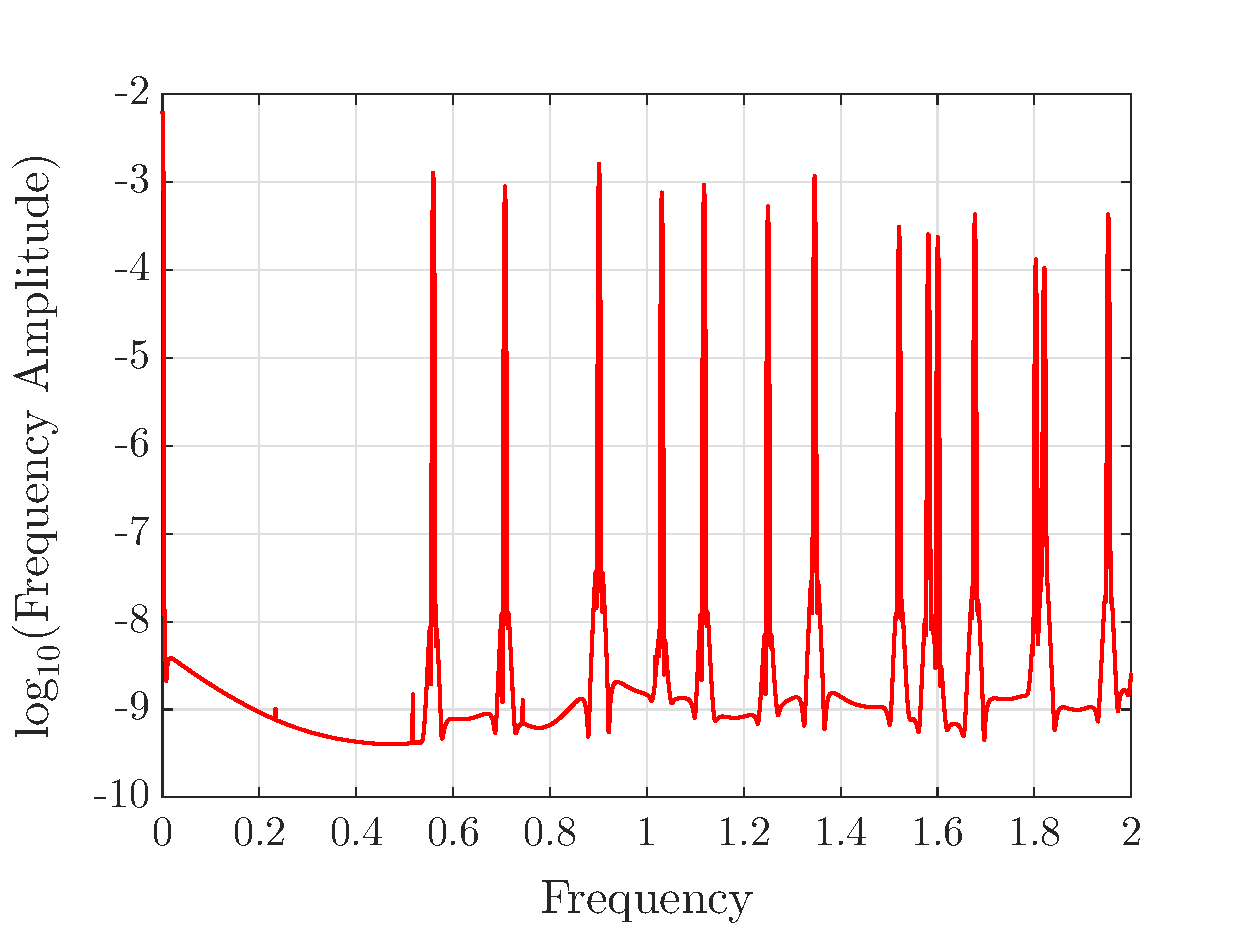
\includegraphics[width=0.49\textwidth]{Windows/spectra/BlackmanHarris-T1000}}
\subfigure[$T=10000$]{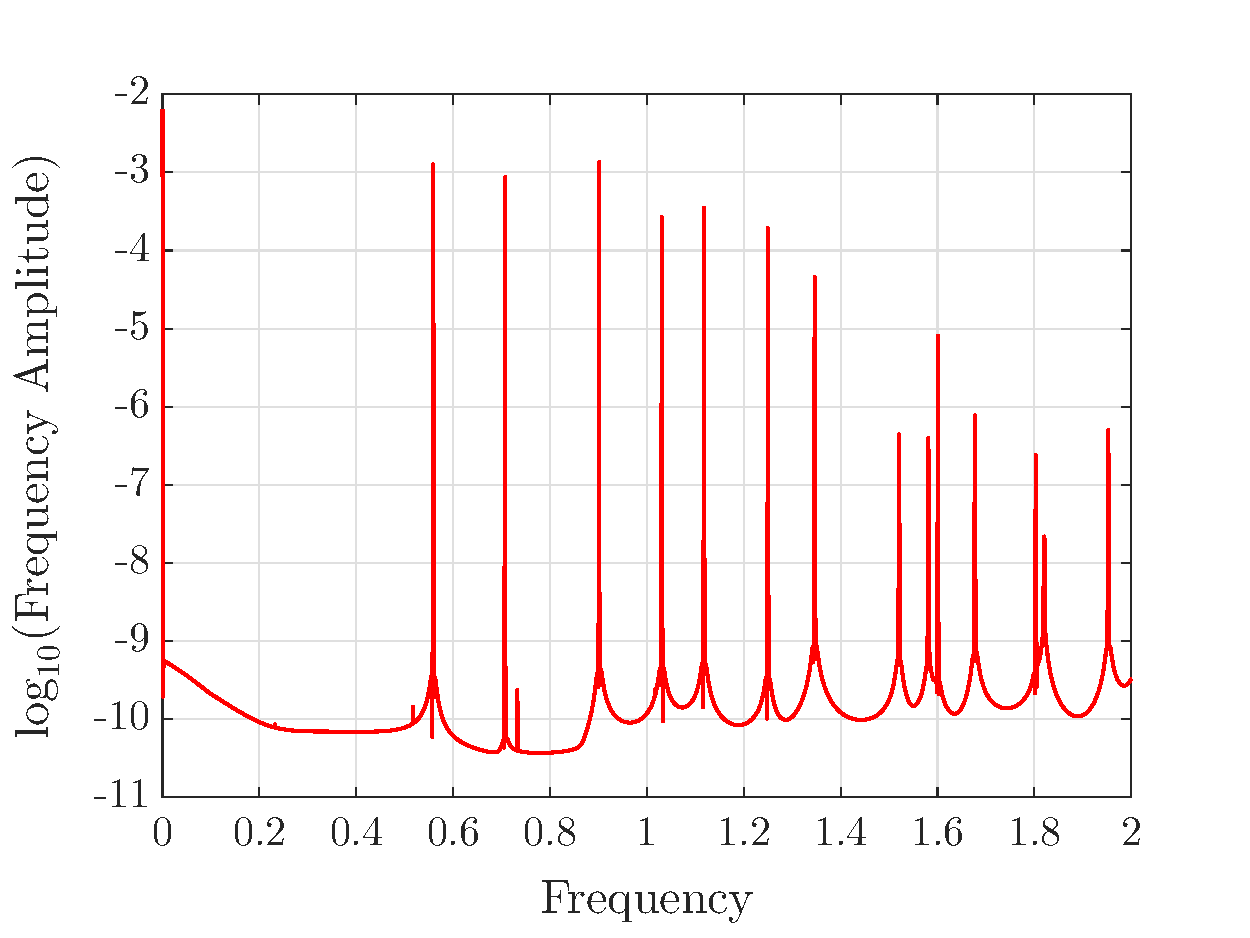
\includegraphics[width=0.49\textwidth]{Windows/spectra/BlackmanHarris-T10000}}
\end{figure}
%figure: DONE various windows (spectra)
\begin{figure}[!ht]
	\centering
\subfigure[ Rectangular window]{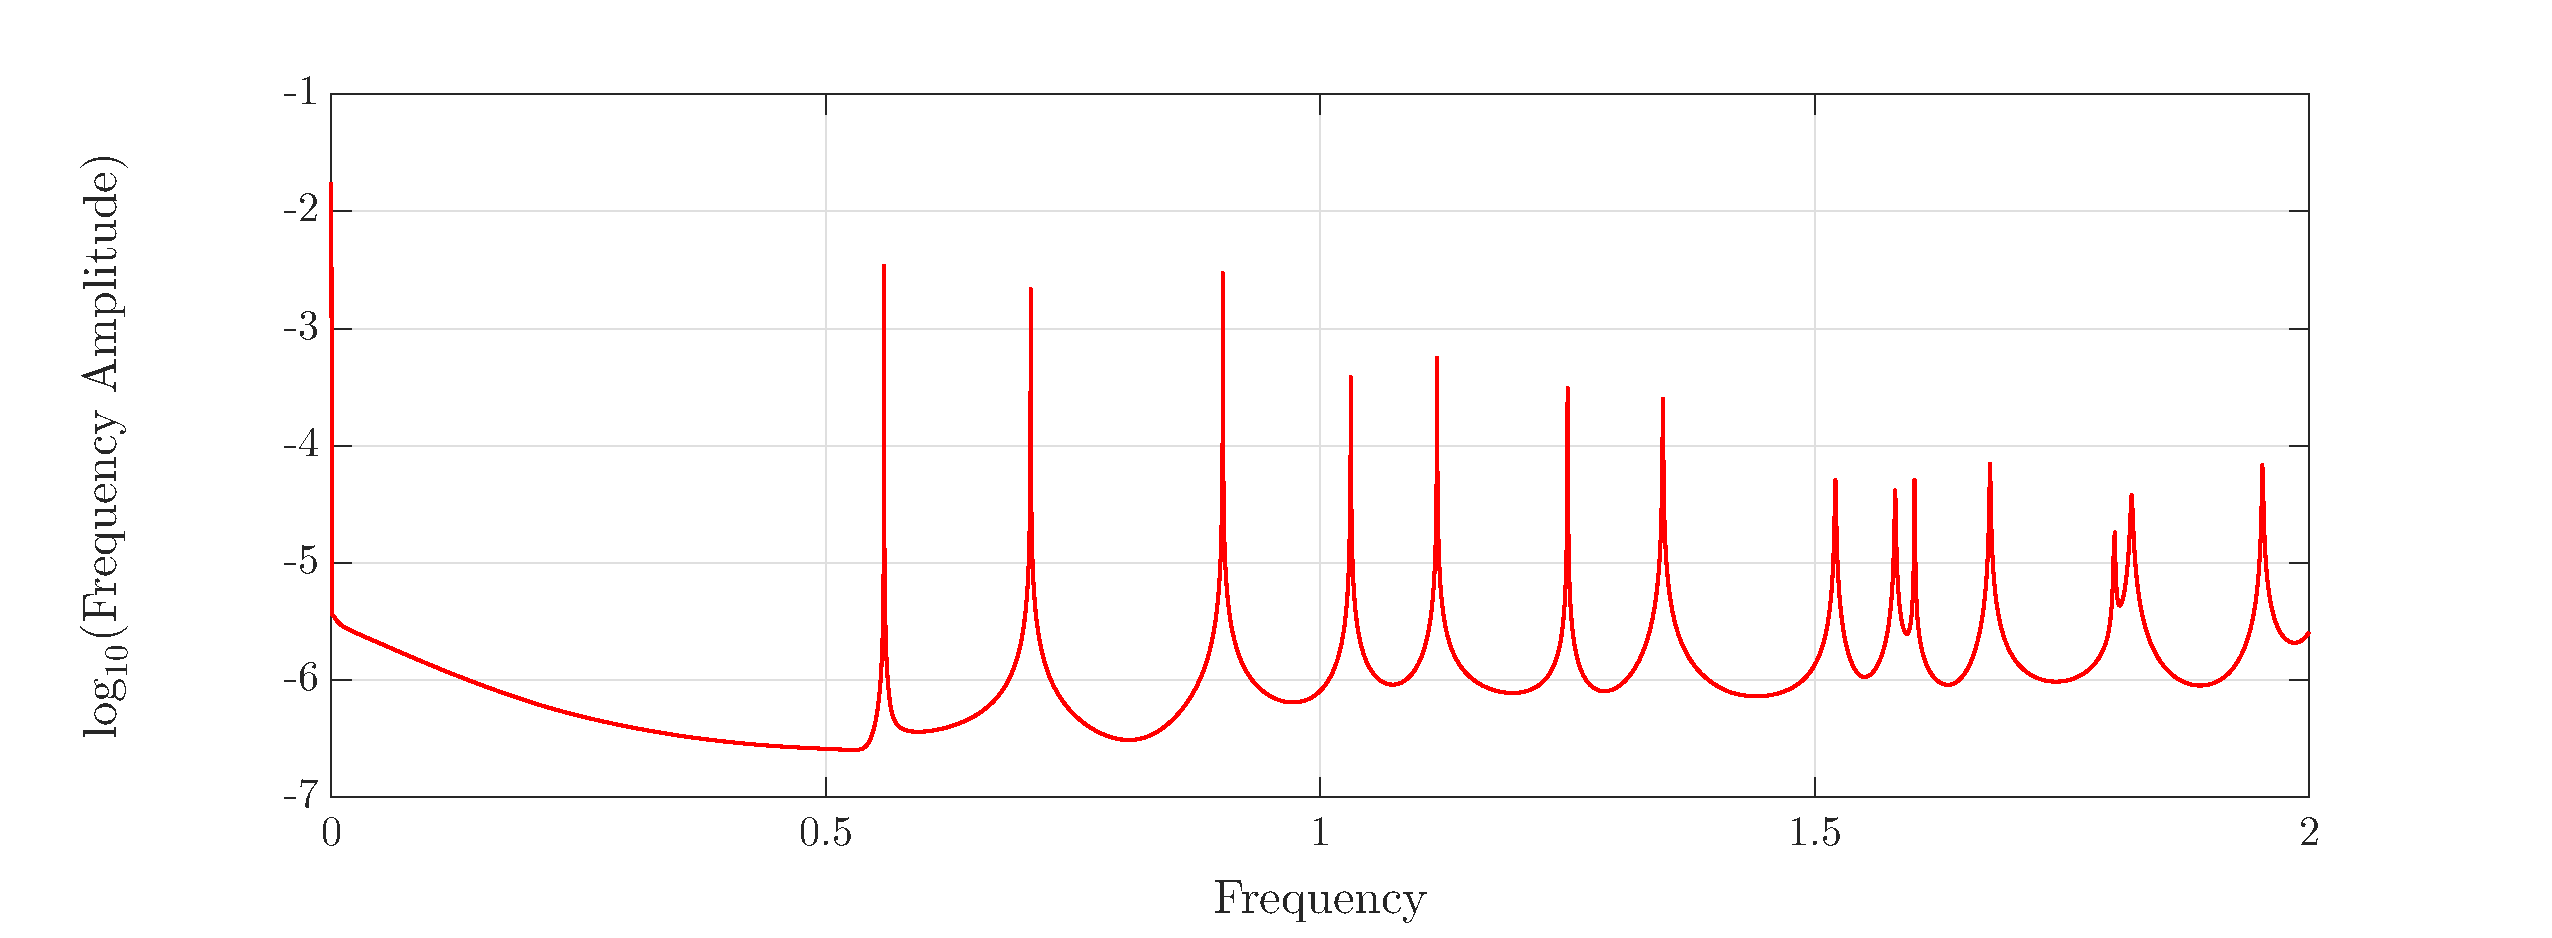
\includegraphics[width=\textwidth]{2D_FreeSpaceCavity/Windows/spectra/RectWindow}}
\subfigure[ Blackman window]{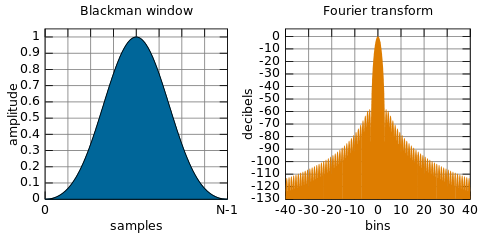
\includegraphics[width=\textwidth]{2D_FreeSpaceCavity/Windows/spectra/BlackmanWindow}}
\subfigure[ Blackman-Harris window]{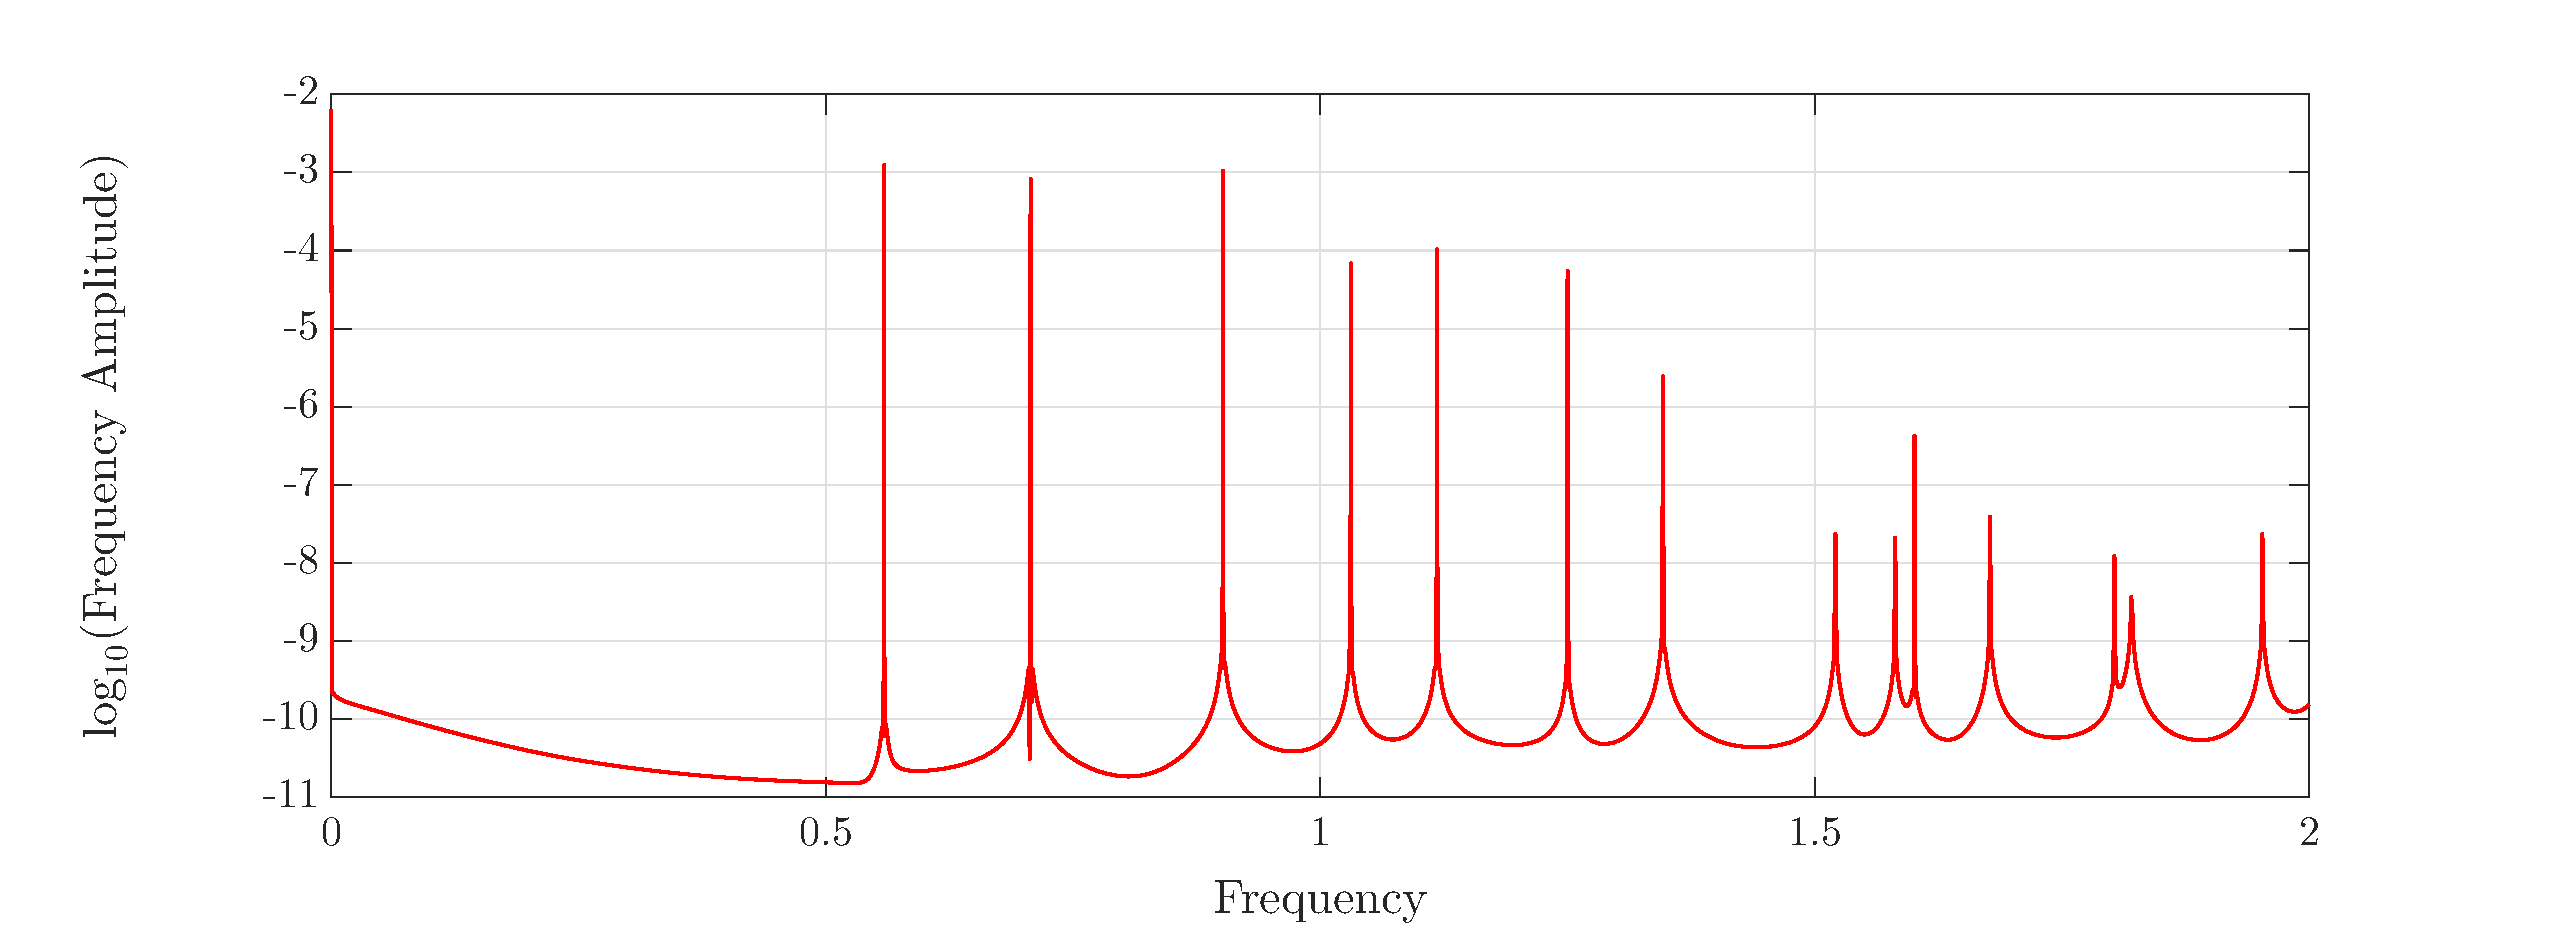
\includegraphics[width=\textwidth]{2D_FreeSpaceCavity/Windows/spectra/BlackmanHarrisWindow}}
\subfigure[ Gaussian window]{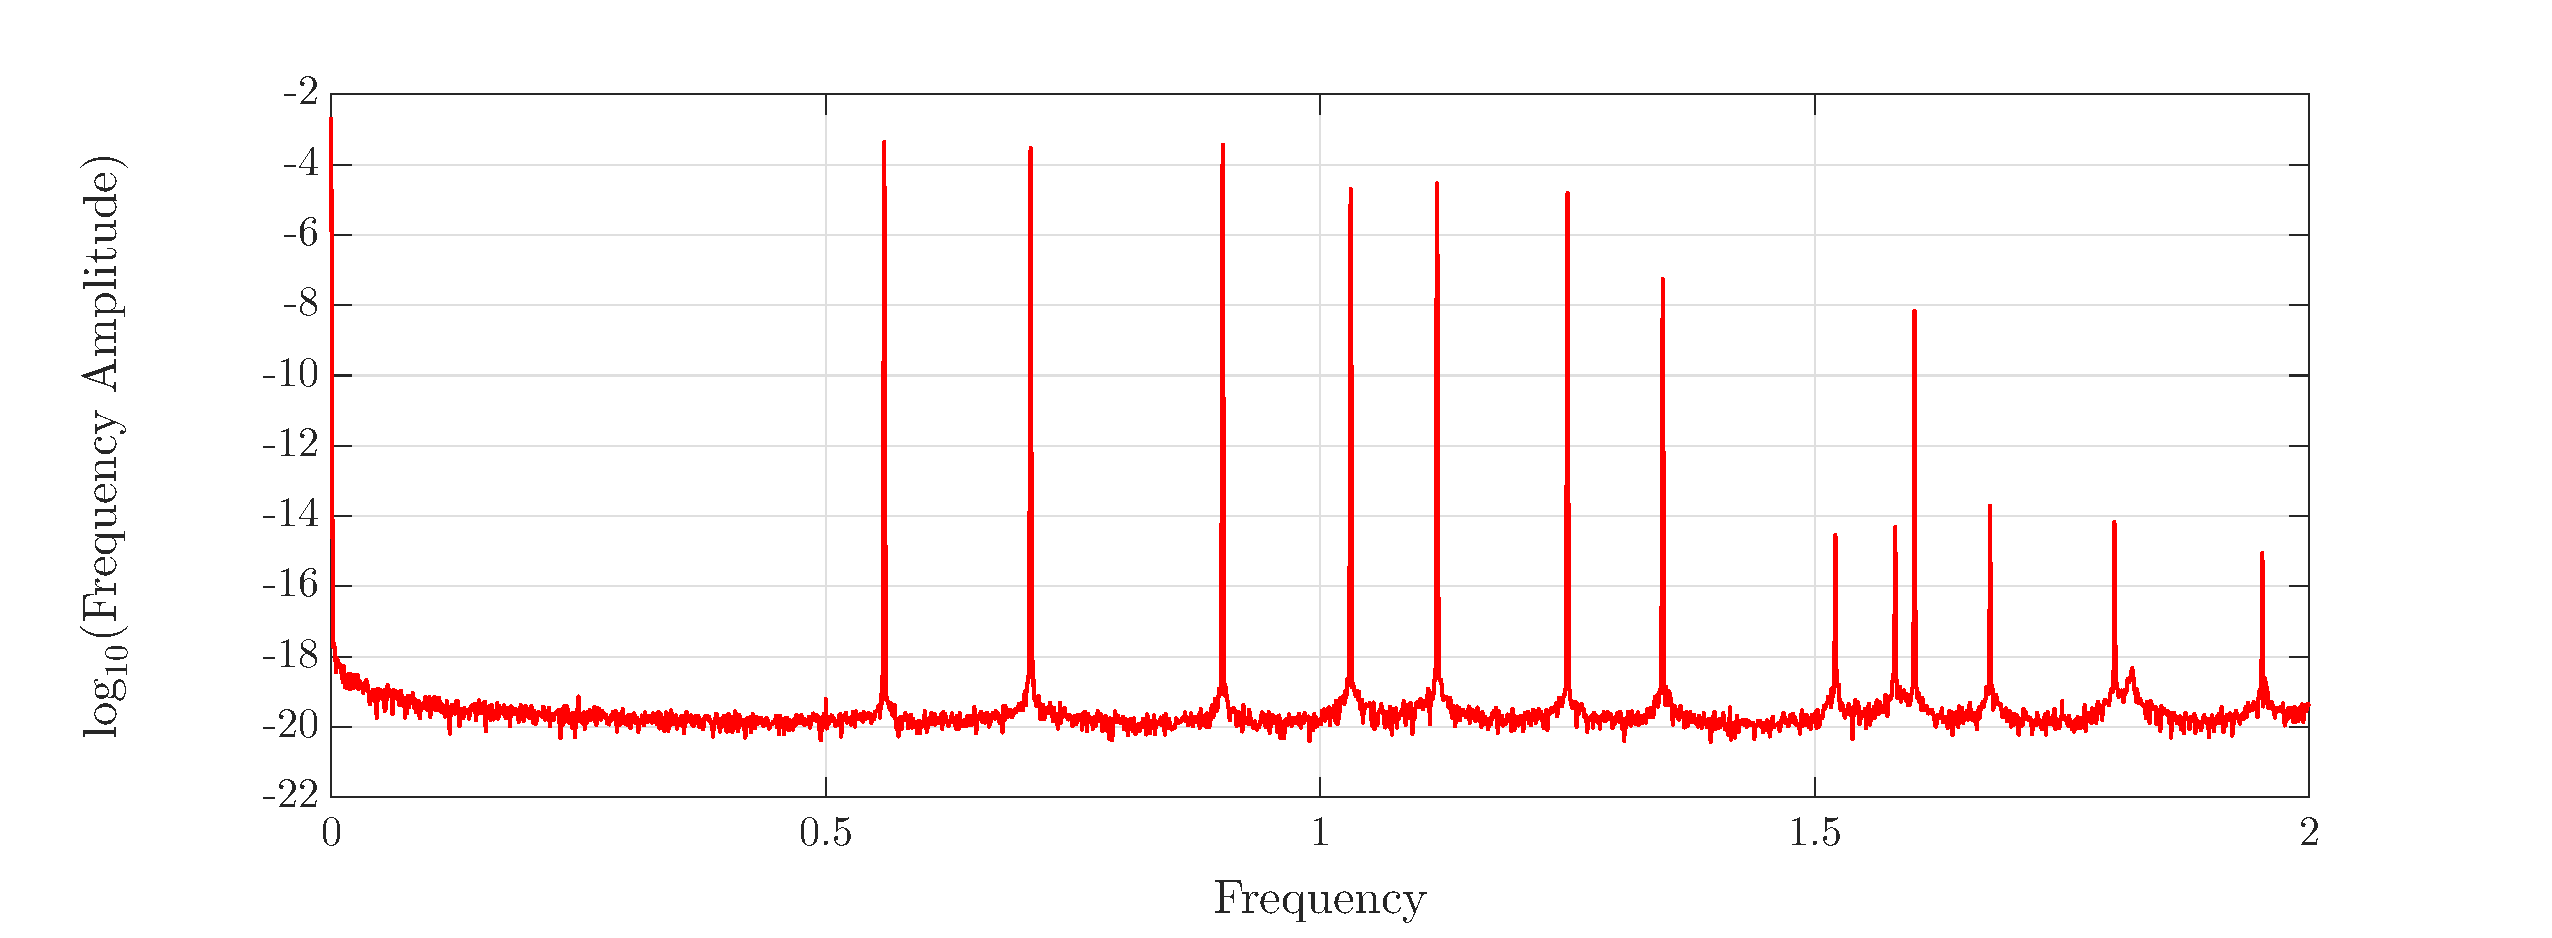
\includegraphics[width=\textwidth]{2D_FreeSpaceCavity/Windows/spectra/GaussianWindow}}
\end{figure}
%figure DONE convergence with various windows
\begin{figure}[!ht]
	\centering
  \subfigure[$f_{3}$]{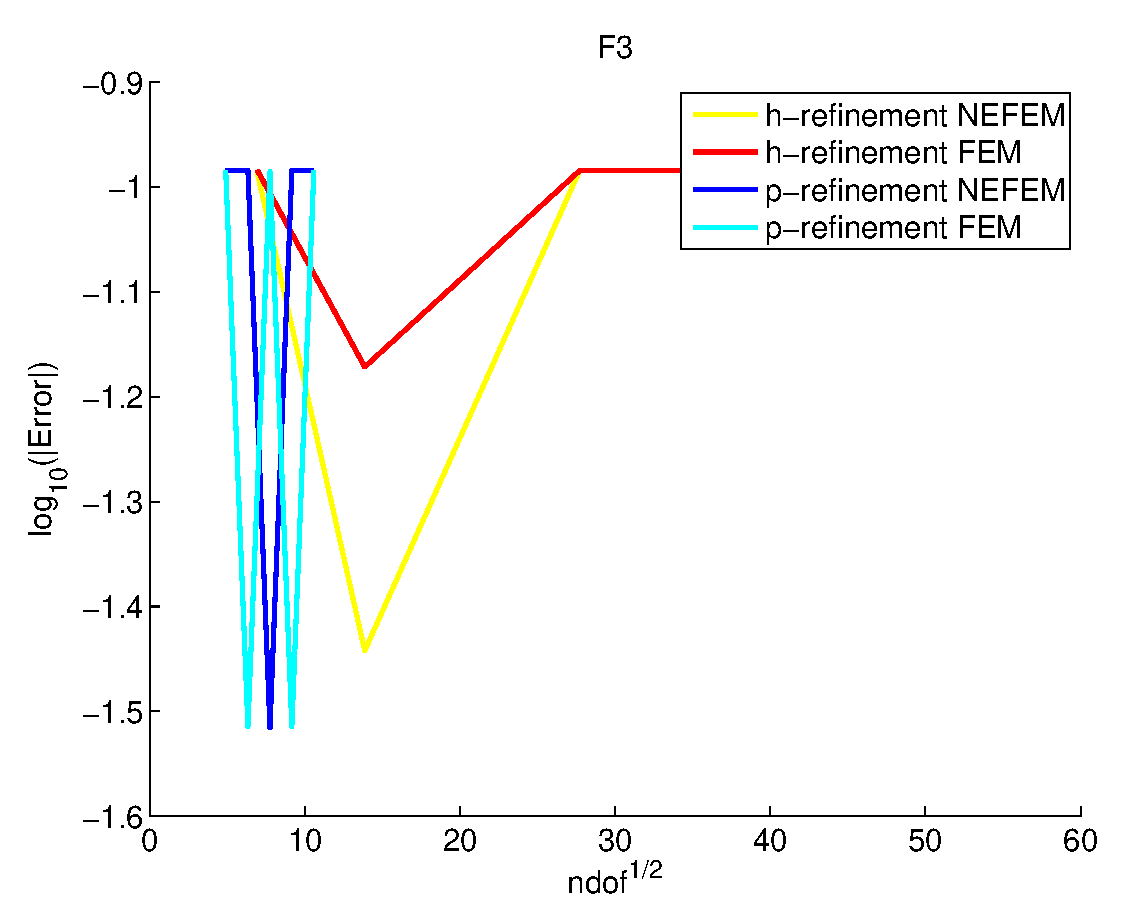
\includegraphics[width=0.45\textwidth]{2D_FreeSpaceCavity/Windows/conv/F3}}
  %\subfigure[$f_{4}$]{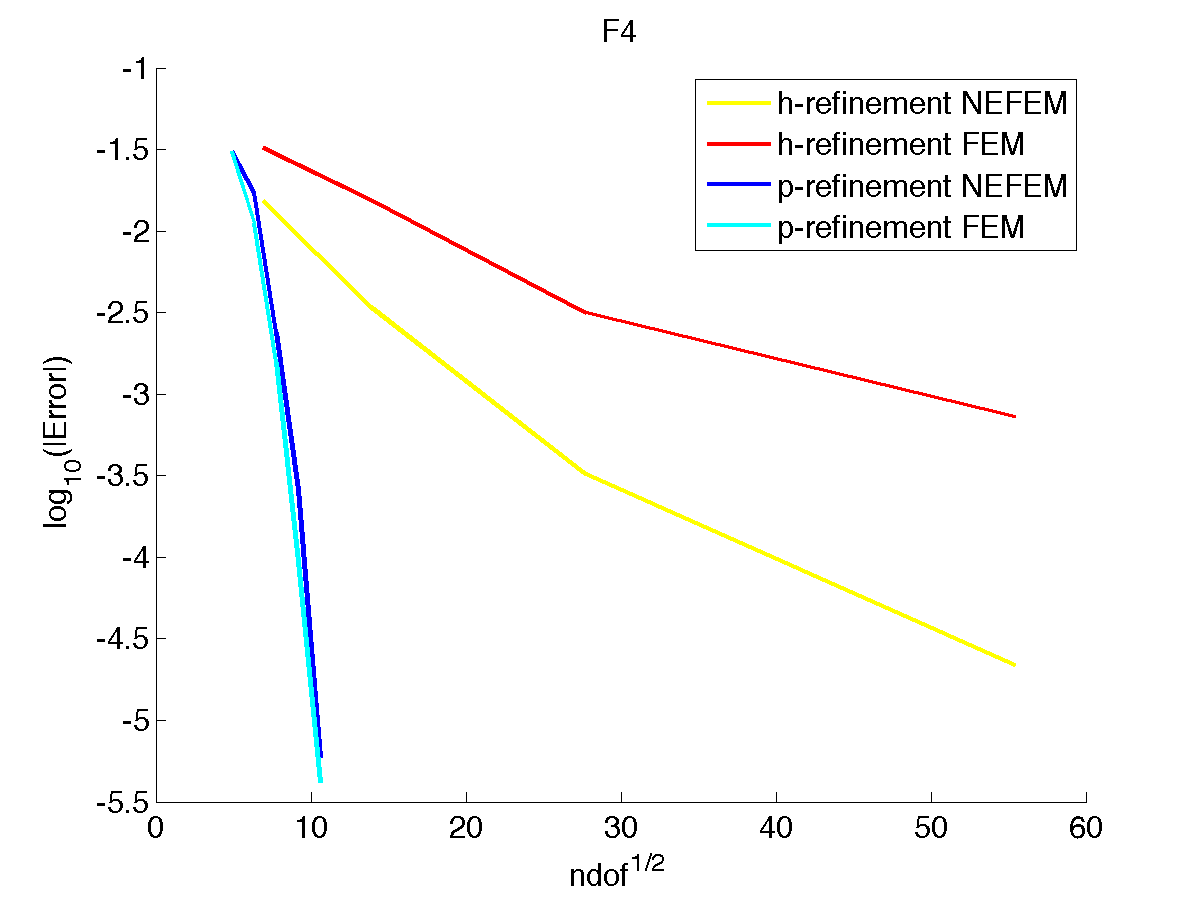
\includegraphics[width=0.45\textwidth]{2D_FreeSpaceCavity/Windows/conv/F4}}
  %\subfigure[$f_{8}$]{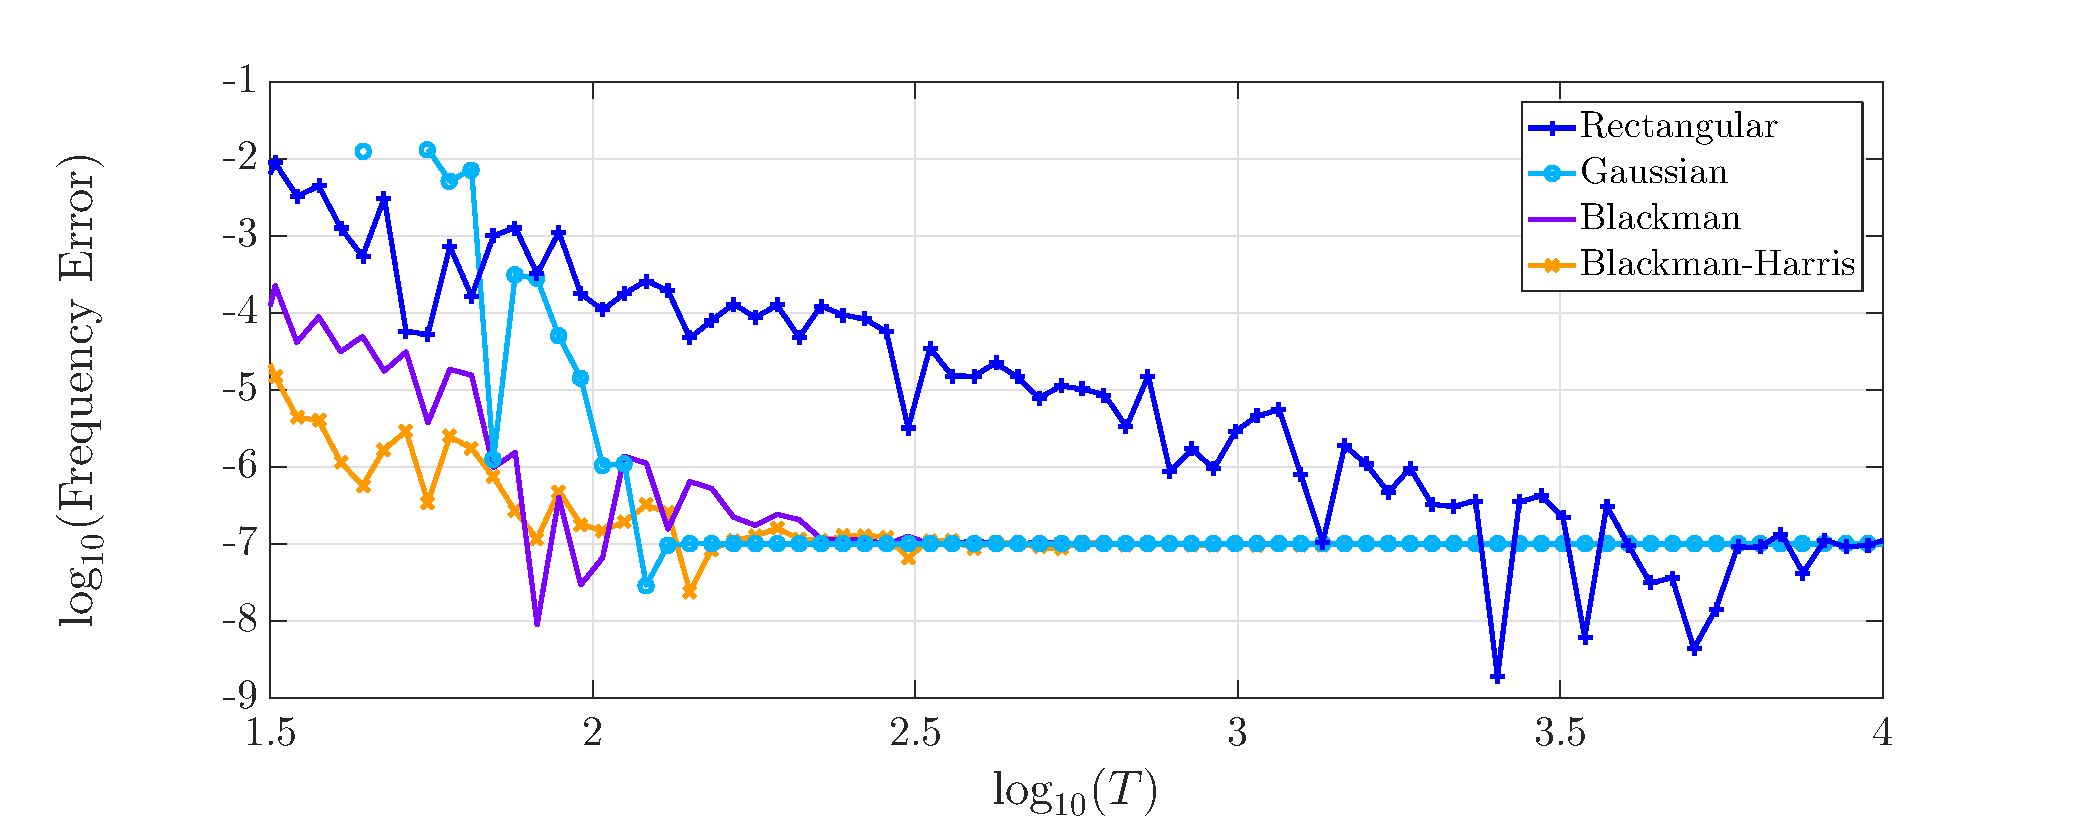
\includegraphics[width=0.45\textwidth]{2D_FreeSpaceCavity/Windows/conv/F8}}
  %\subfigure[$f_{9}$]{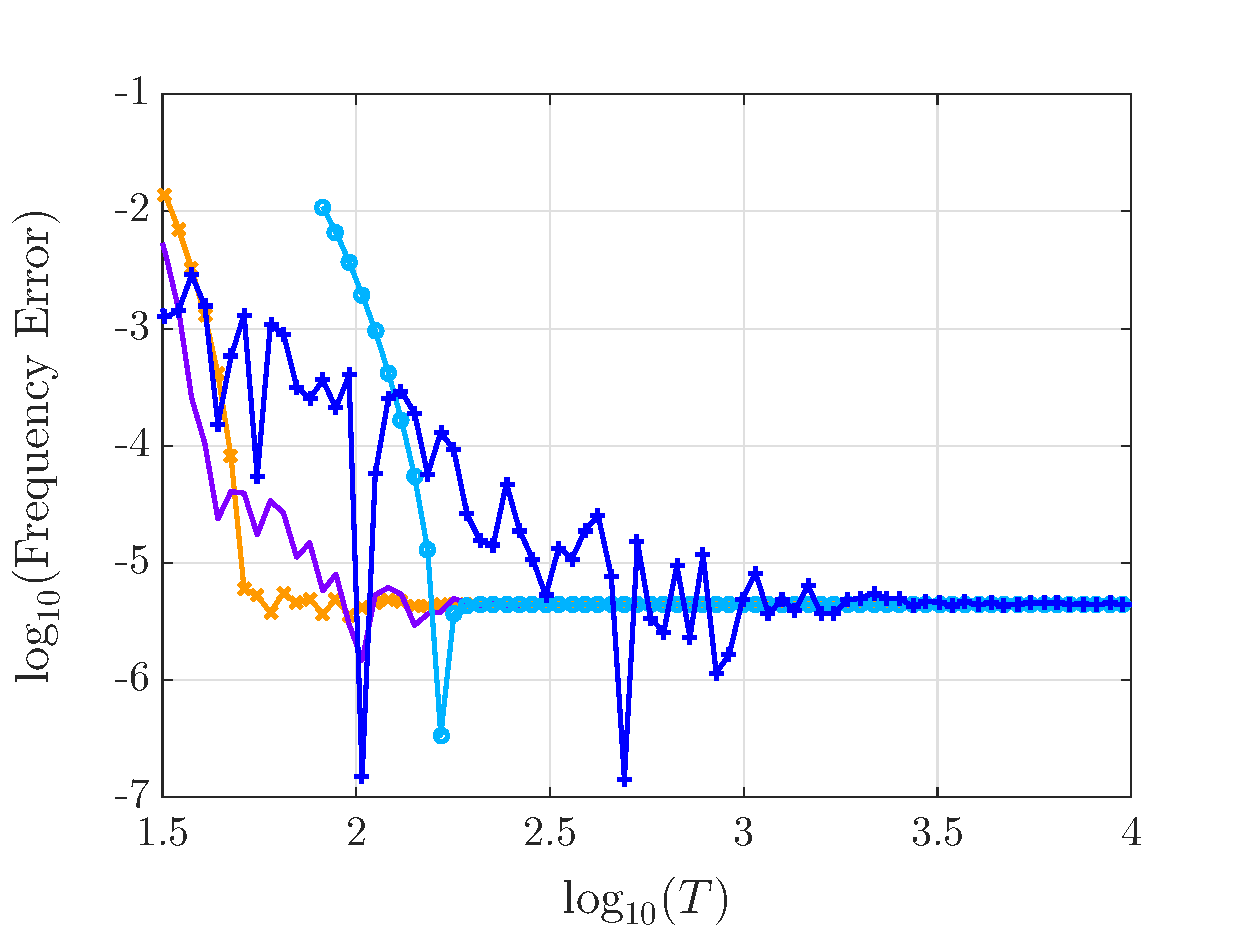
\includegraphics[width=0.45\textwidth]{2D_FreeSpaceCavity/Windows/conv/F9}}
  \subfigure[$f_{10}$]{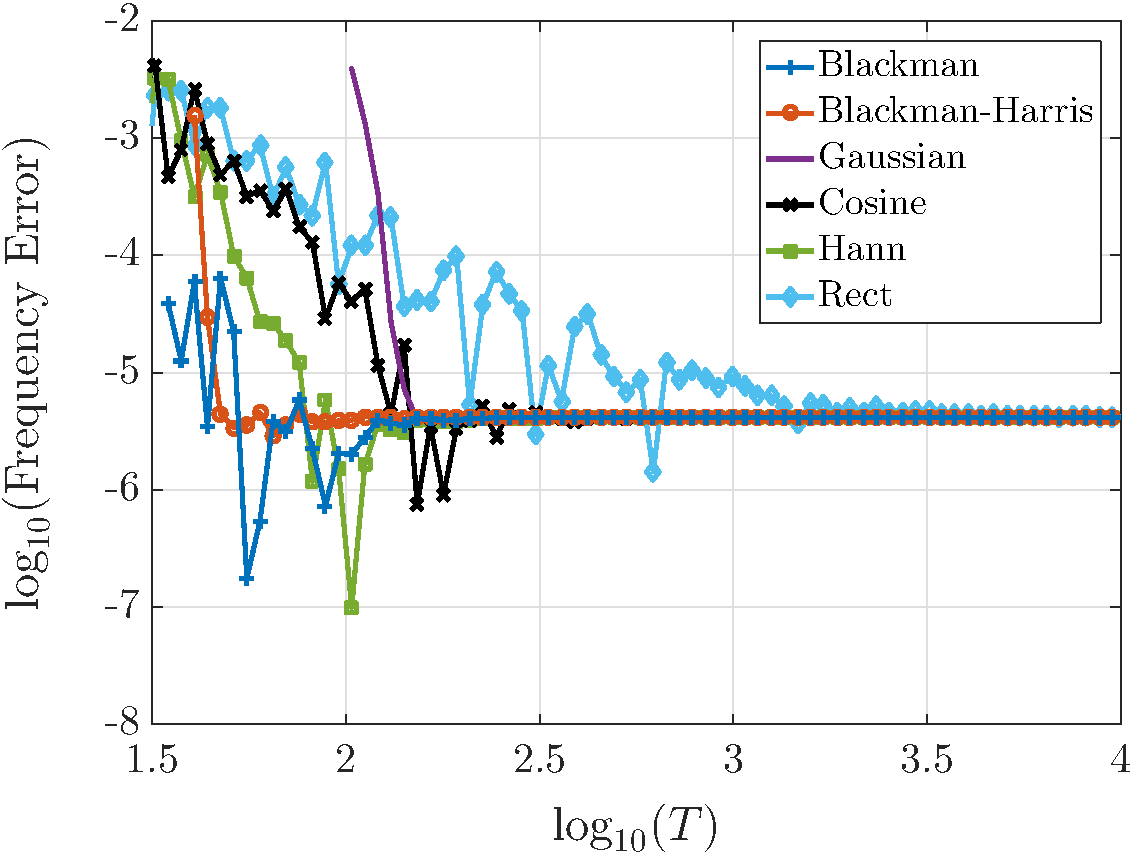
\includegraphics[width=0.45\textwidth]{2D_FreeSpaceCavity/Windows/conv/F10_legend}}
	\label{fig:rectangle2DfreeSpace_filteringConvergence}
\end{figure}
\clearpage
\subsection{Effect of the geometric representation for cavities with curved boundaries}
%text
The second example considers the computation of the resonant frequencies and associated modes in a metallic disk resonator of radius 1$\mu$m filled with air, for which an analytical solution is known~\cite{BalanisBook}. The objective is to study the effect of the geometric approximation of curved boundaries in the accuracy and convergence properties of isoparametric finite elements and NEFEM. In addition, the benefits of using high-order curved elements in this context are quantified using the computational time. 

The resonator is discretised using a series of unstructured triangular meshes with 4, 16, 64, 256, and 1,024 elements and with different orders of approximation. Figure~\ref{fig:circleFEMvsNEFEM_Convergence} (a) shows the evolution of the error in the first resonant frequency, $f_1 \approx$ 57.59 THz, as a function of the element size for linear and quadratic elements and by using standard isoparametric finite elements and NEFEM. 
%figure REVISE - 2D Circle convergence comparison - more of them!
\begin{figure}[!ht]
	\centering
	\subfigure[$h$-refinement]{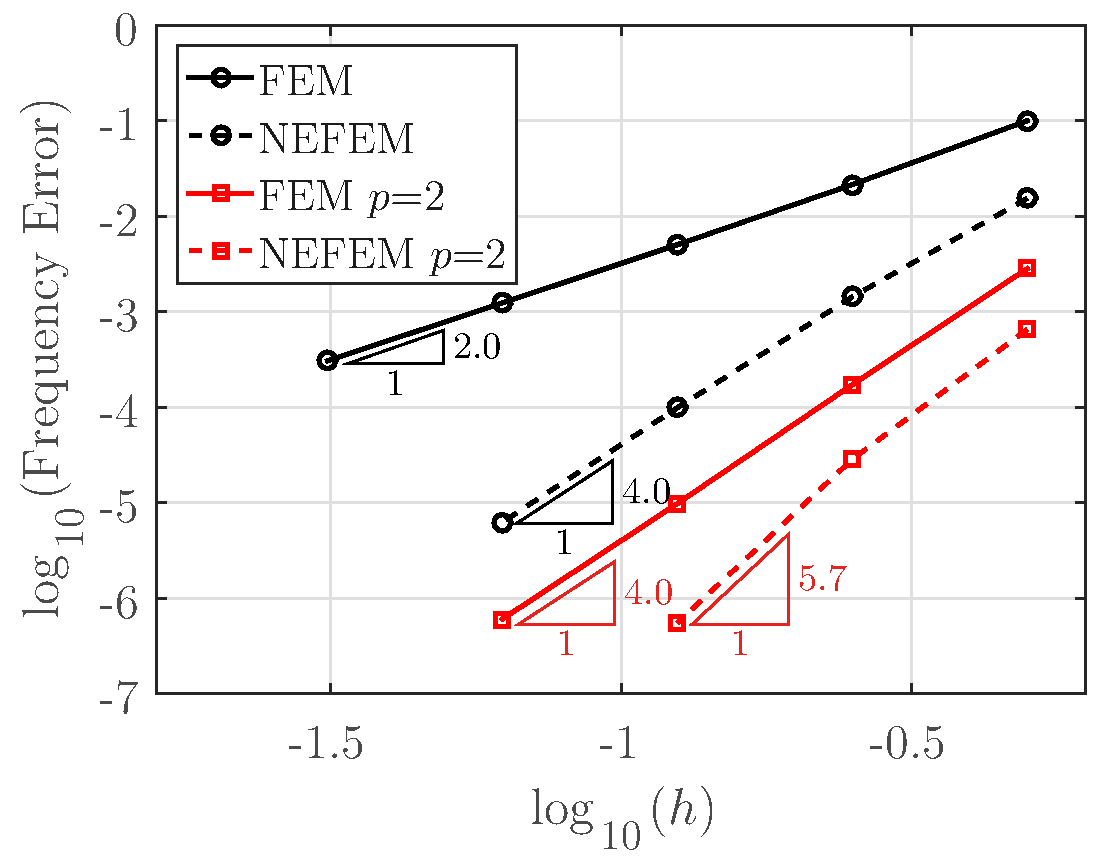
\includegraphics[width=0.49\textwidth]{figs/circleFreeSpace_hRef}}
	\subfigure[$p$-refinement]{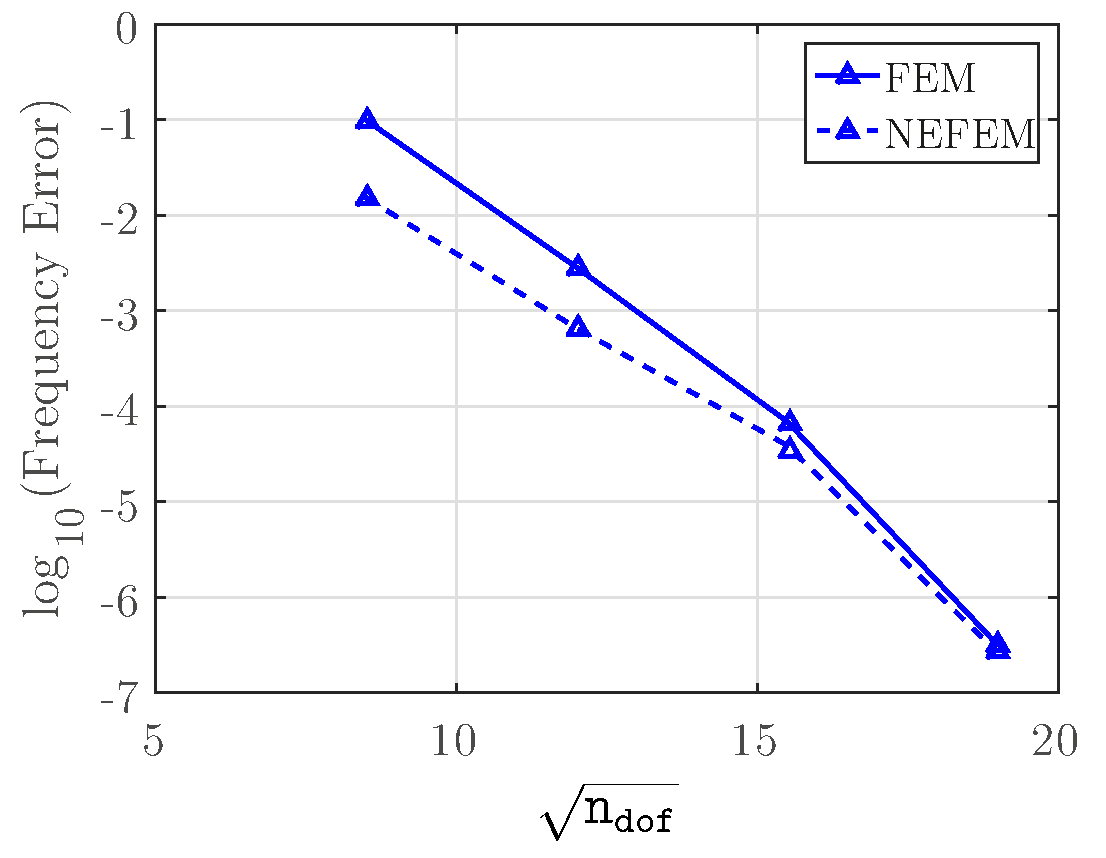
\includegraphics[width=0.49\textwidth]{figs/circleFreeSpace_pRef}}
	\caption{Disk resonator: $h$-convergence and $p$-convergence of the error for the first resonant frequency $f_1 \approx$ 57.59 THz.}
	\label{fig:circleFEMvsNEFEM_Convergence}
\end{figure}
%text
The results show that the geometric approximation of curved boundaries introduced by standard finite elements induce not only a significant loss of accuracy but, more importantly, a loss of the optimal rate of convergence. For example, in the fourth mesh, with 256 elements and using a linear approximation of the solution, the error on the resonant frequency with NEFEM is more than two orders of magnitude lower than the error obtained by using standard finite elements. For isoparametric finite element a rate of convergence $2p$ is observed whereas for NEFEM the optimal rate of convergence, $2p+2$, is observed. 

Figure~\ref{fig:circleFEMvsNEFEM_Convergence} (b) shows a $p$-refinement study. The first mesh, with only four elements, is considered and the degree of approximation is increased from $p$=1 to $p$=4. The evolution of the error in the first resonant frequency as a function of the square root of the number of degrees of freedom is shown for isoparametric finite elements and NEFEM. The comparison shows important differences for low order approximations (i.e, $p$=1,2) whereas for higher order approximations (i.e, $p \geq$3), a similar error is obtained suggesting that a high order approximation of the geometry is mandatory is order to avoid an effect on the computed resonant frequencies. 

Figure~\ref{fig:circle2DfreeSpace_modes} shows the third component of the electric field for twelve modes. 
%figure DONE Circle Mode Shapes
\begin{figure}[!ht]
\centering
\subfigure[$f_1 \approx$ 57.37 THz]{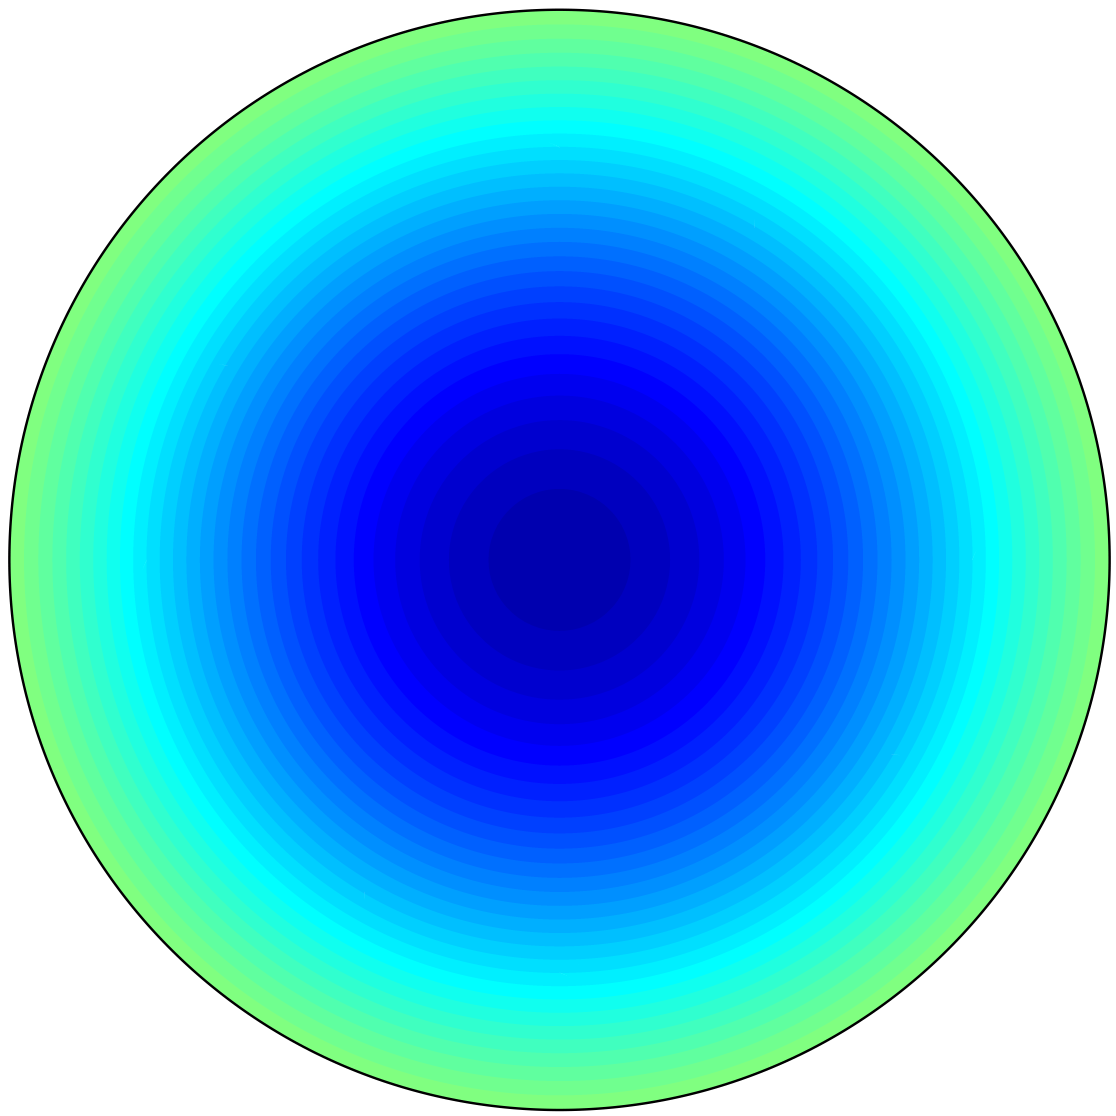
\includegraphics[width=0.24\textwidth] {2D_Circle/modeShapes/circleFreeSpace_mode1_U3}}
\subfigure[$f_2 \approx$ 91.41 THz]{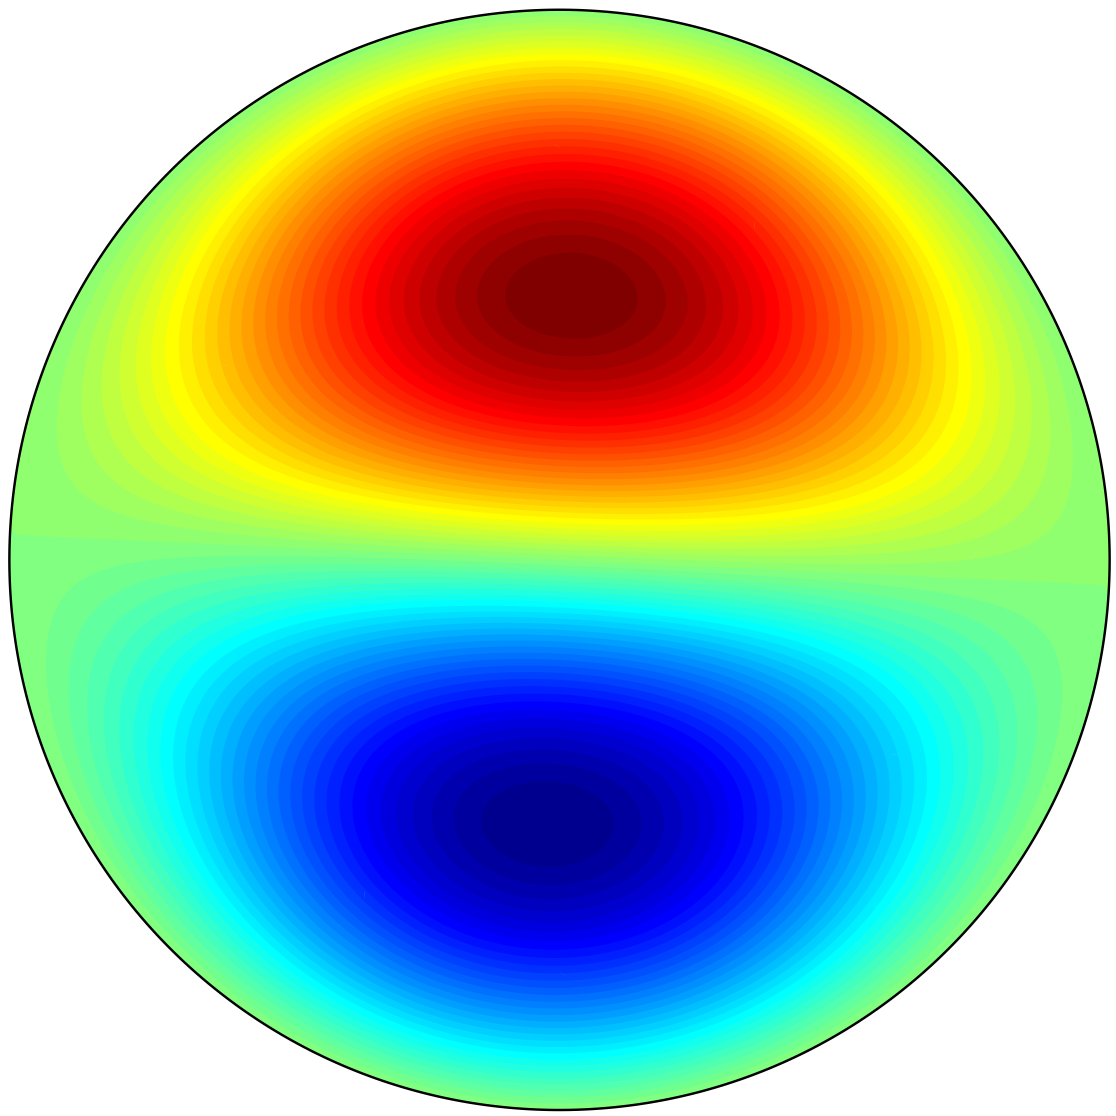
\includegraphics[width=0.24\textwidth] {2D_Circle/modeShapes/circleFreeSpace_mode2_U3}}
\subfigure[$f_3 \approx$ 122.52 THz]{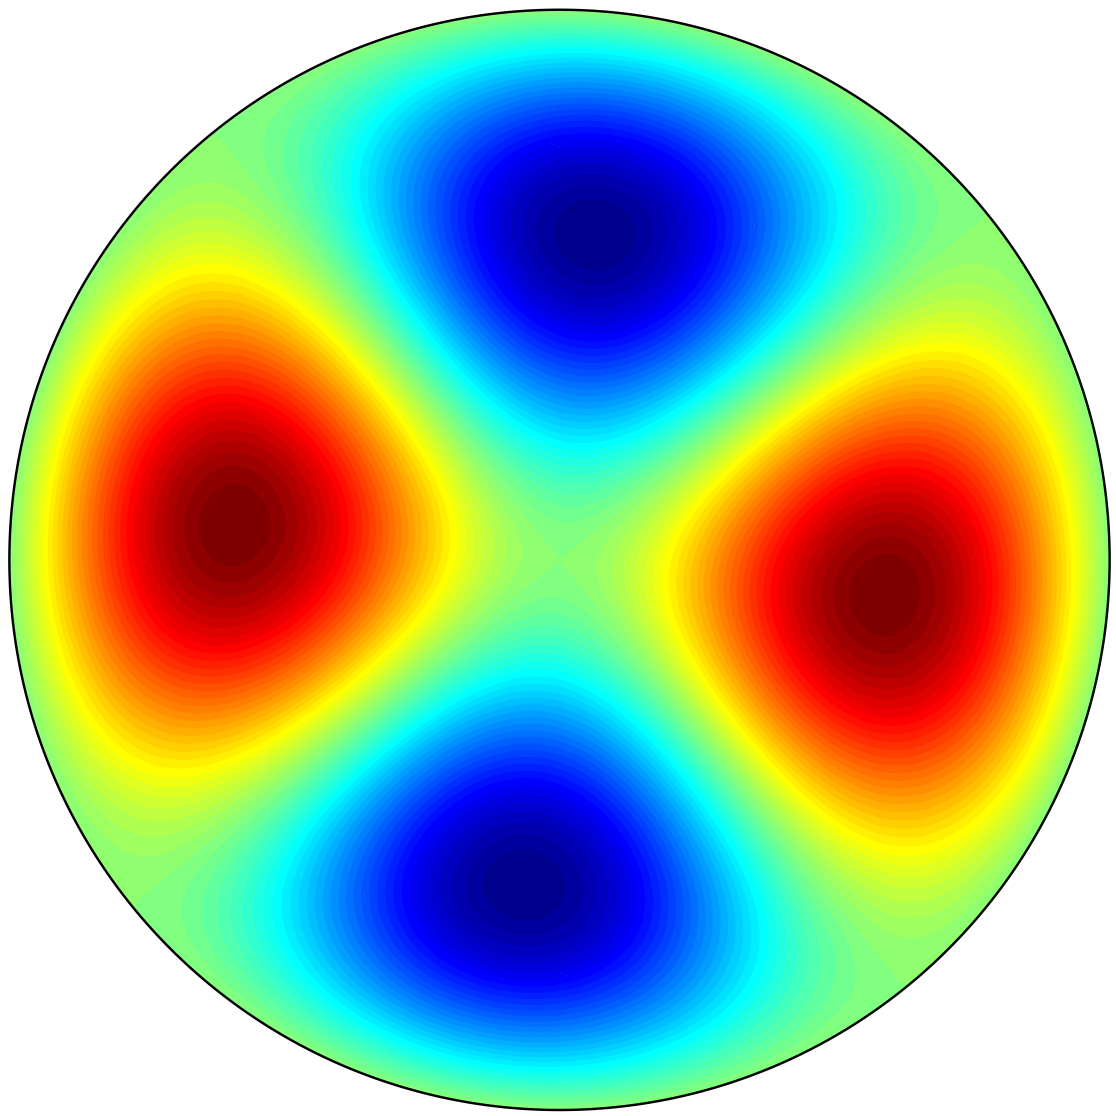
\includegraphics[width=0.24\textwidth] {2D_Circle/modeShapes/circleFreeSpace_mode3_U3}}
\subfigure[$f_{14} \approx$ 263.97 THz]{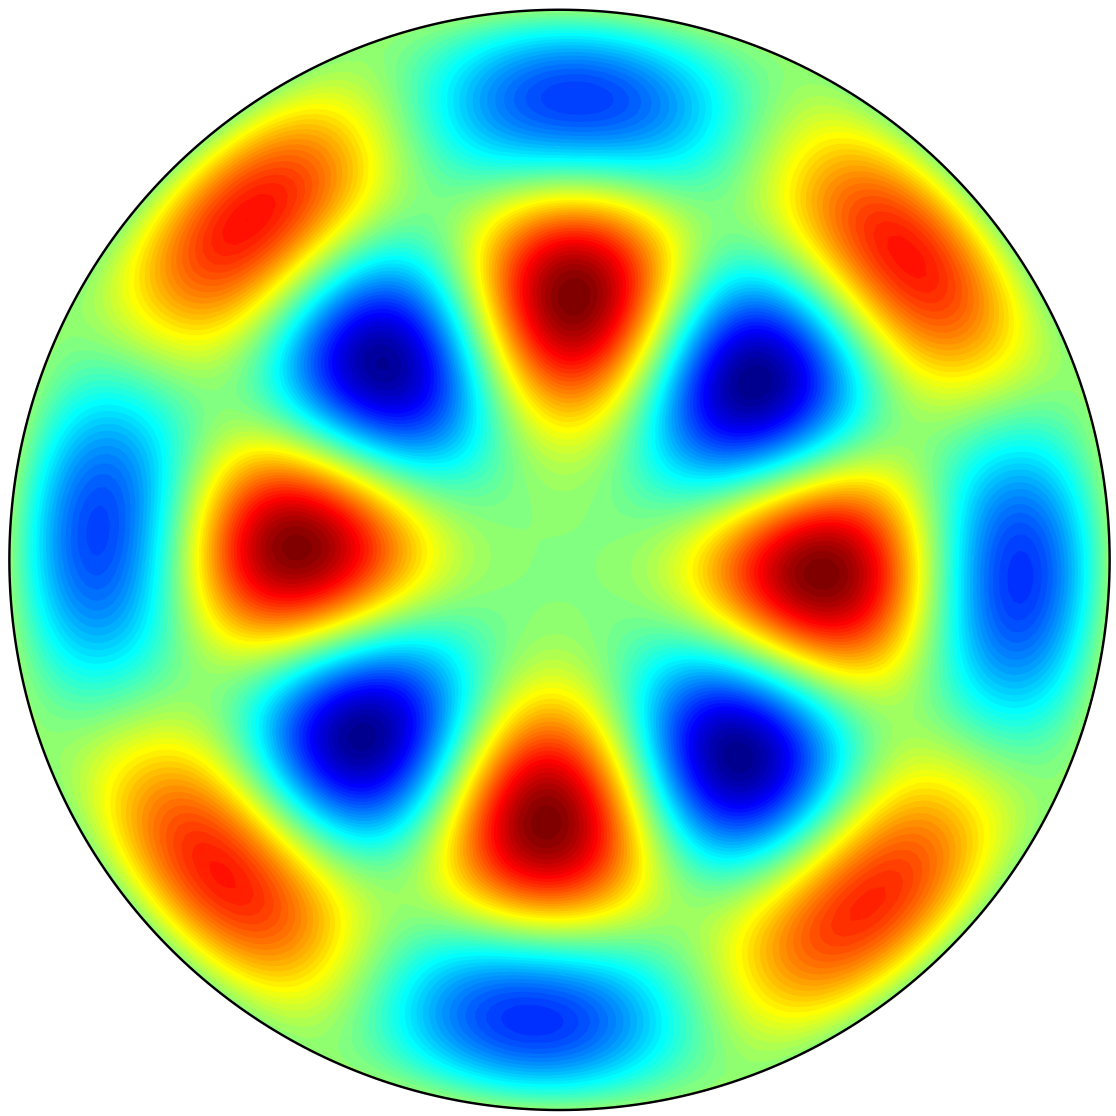
\includegraphics[width=0.24\textwidth] {2D_Circle/modeShapes/circleFreeSpace_mode14_U3}} \\
%
\subfigure[$f_4 \approx$ 131.69 THz]{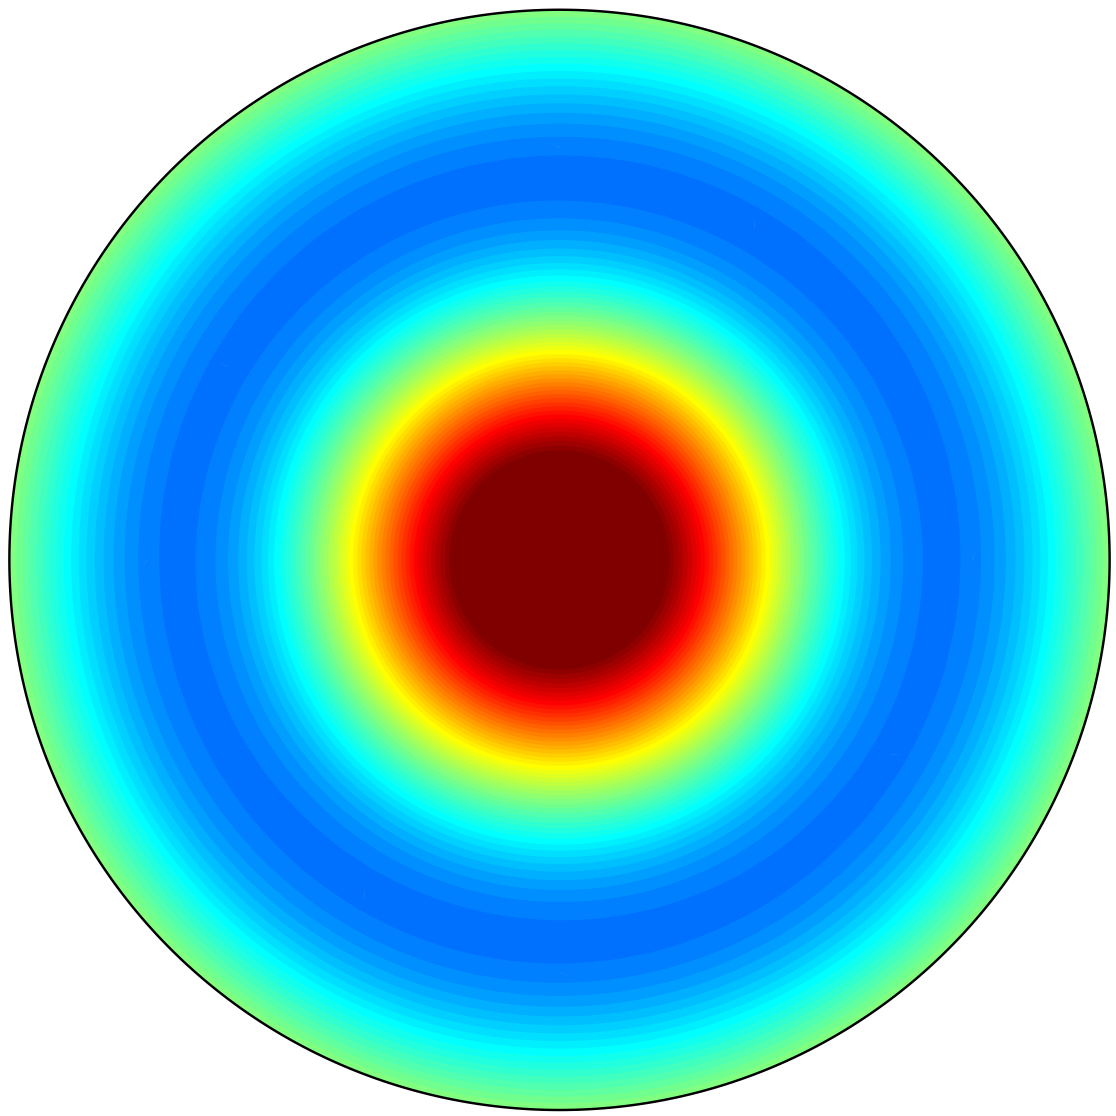
\includegraphics[width=0.24\textwidth] {2D_Circle/modeShapes/circleFreeSpace_mode4_U3}}
\subfigure[$f_6 \approx$ 167.37 THz]{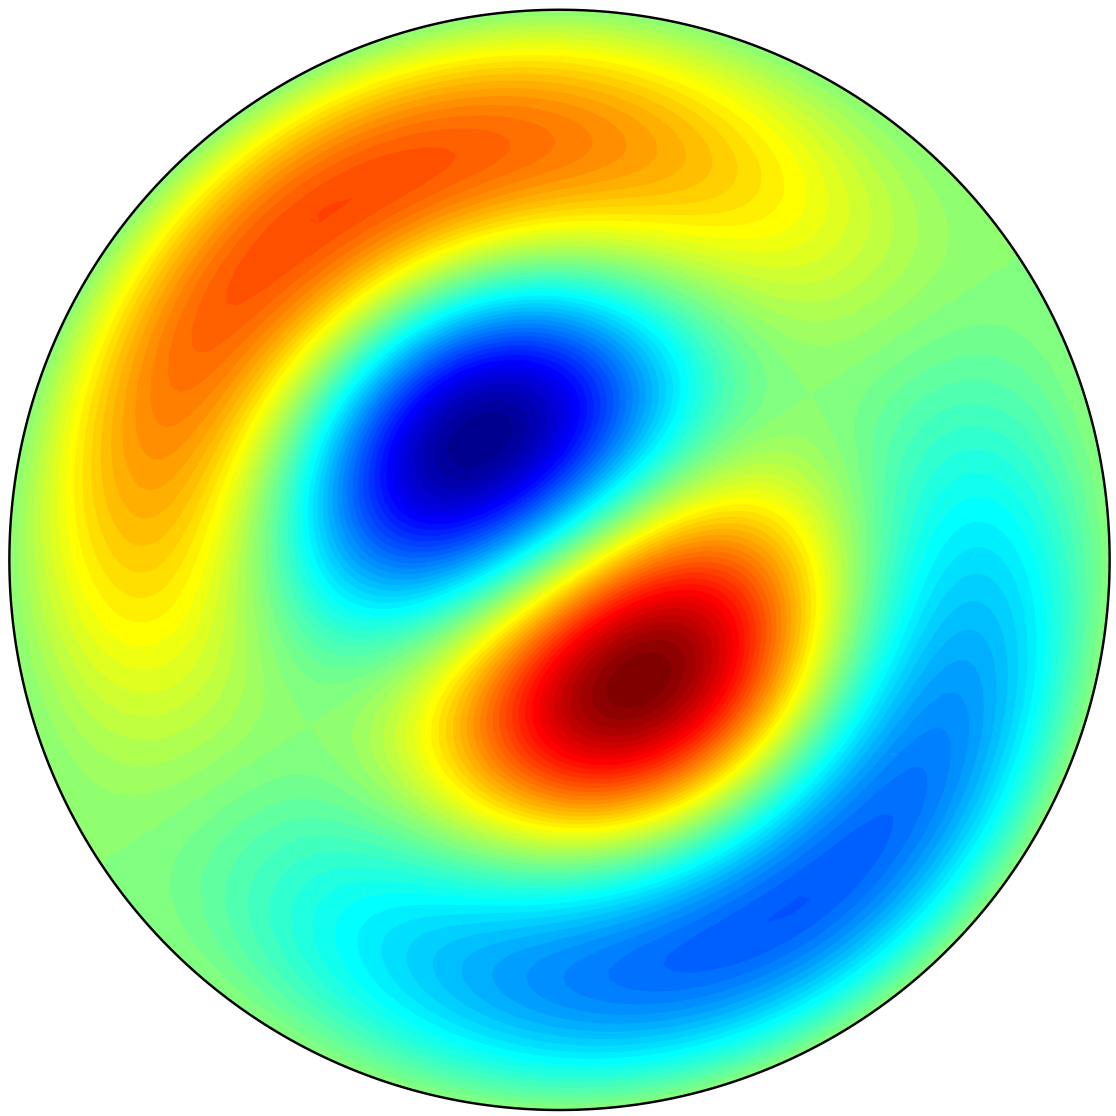
\includegraphics[width=0.24\textwidth] {2D_Circle/modeShapes/circleFreeSpace_mode6_U3}}
\subfigure[$f_5 \approx$ 152.21 THz]{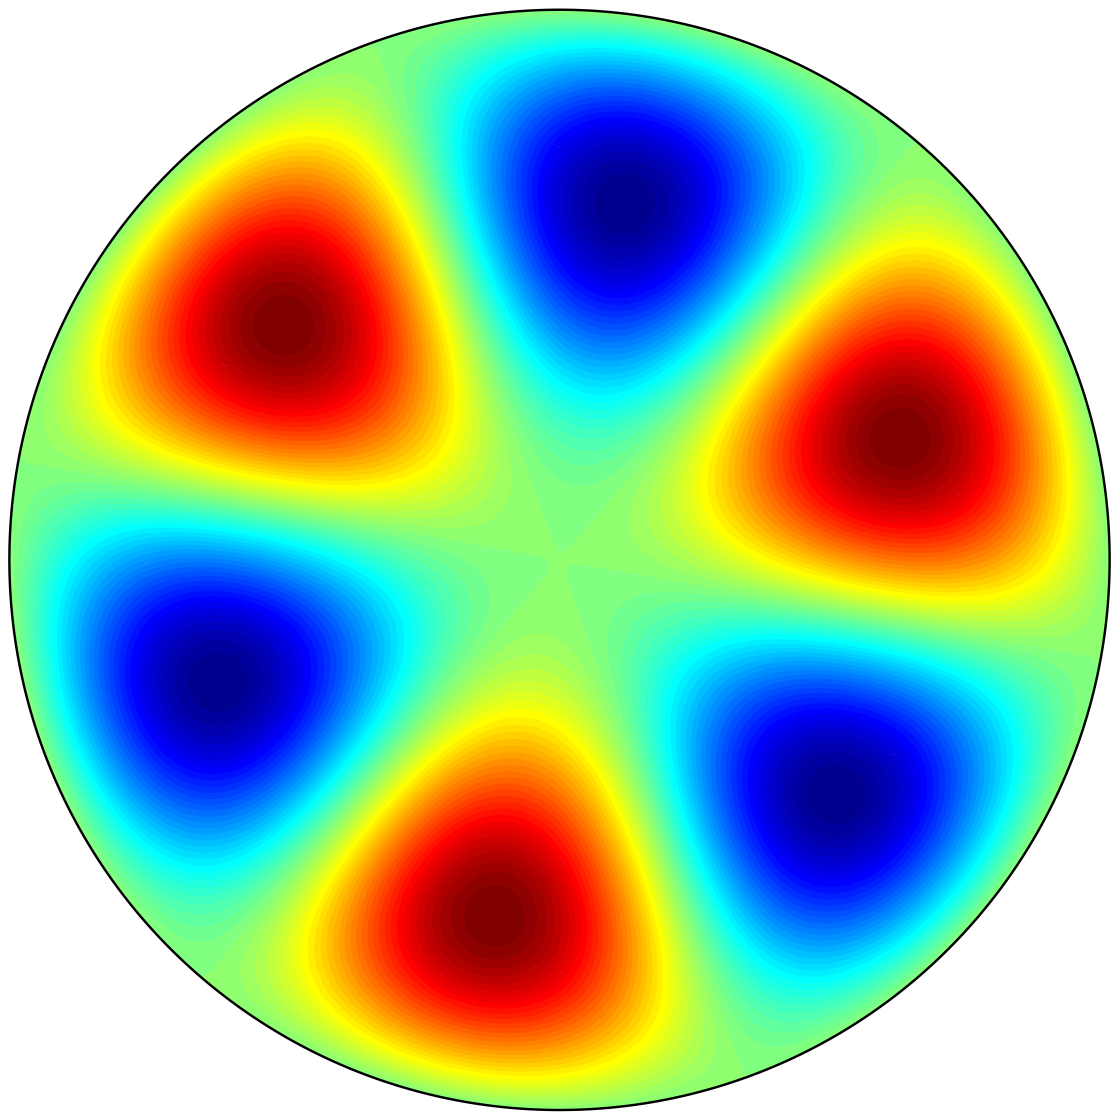
\includegraphics[width=0.24\textwidth] {2D_Circle/modeShapes/circleFreeSpace_mode5_U3}}
\subfigure[$f_{19} \approx$ 294.36 THz]{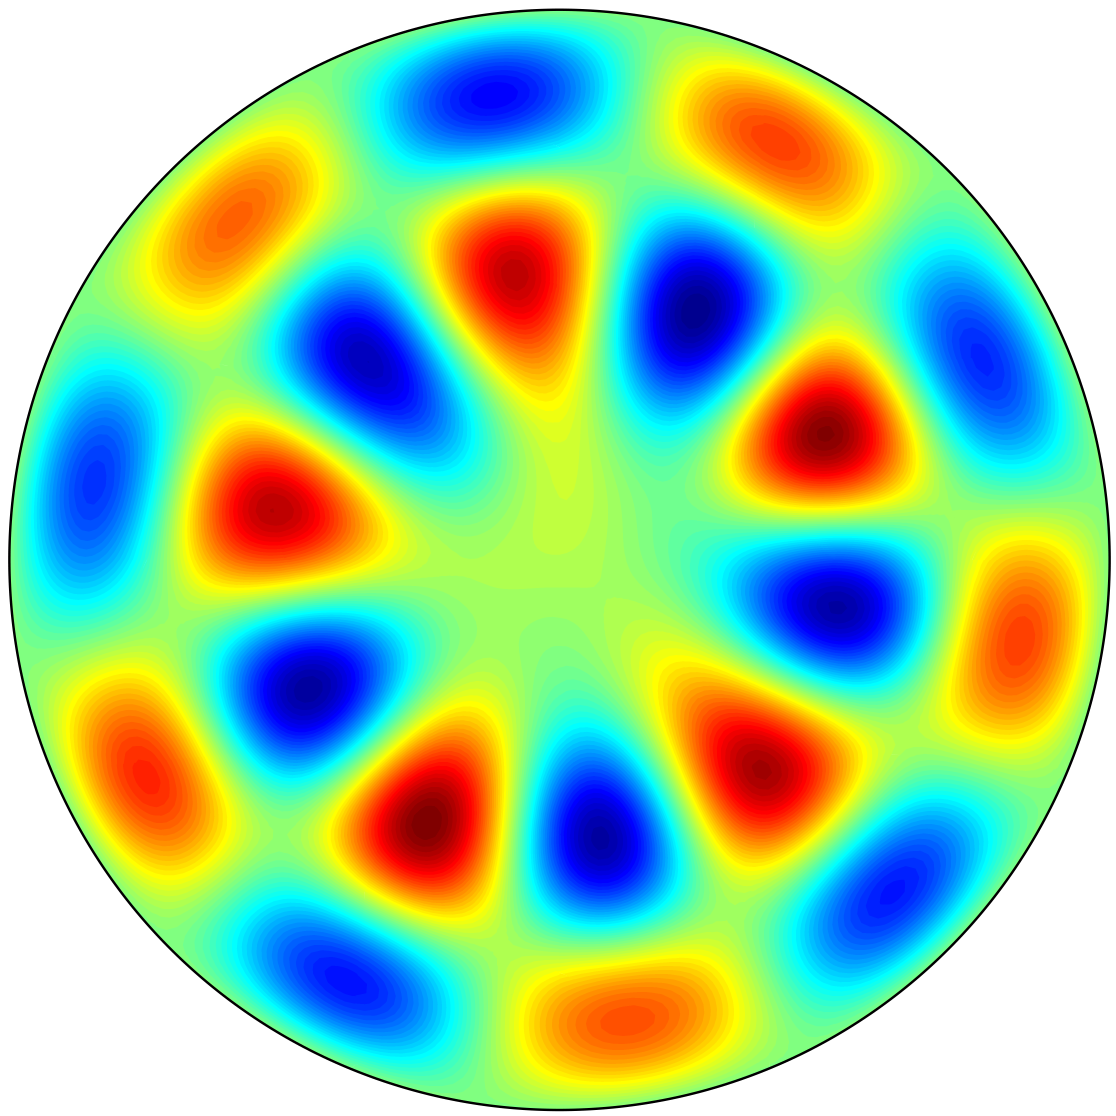
\includegraphics[width=0.24\textwidth] {2D_Circle/modeShapes/circleFreeSpace_mode19_U3}} \\
%
\subfigure[$f_{17} \approx$ 281.31 THz]{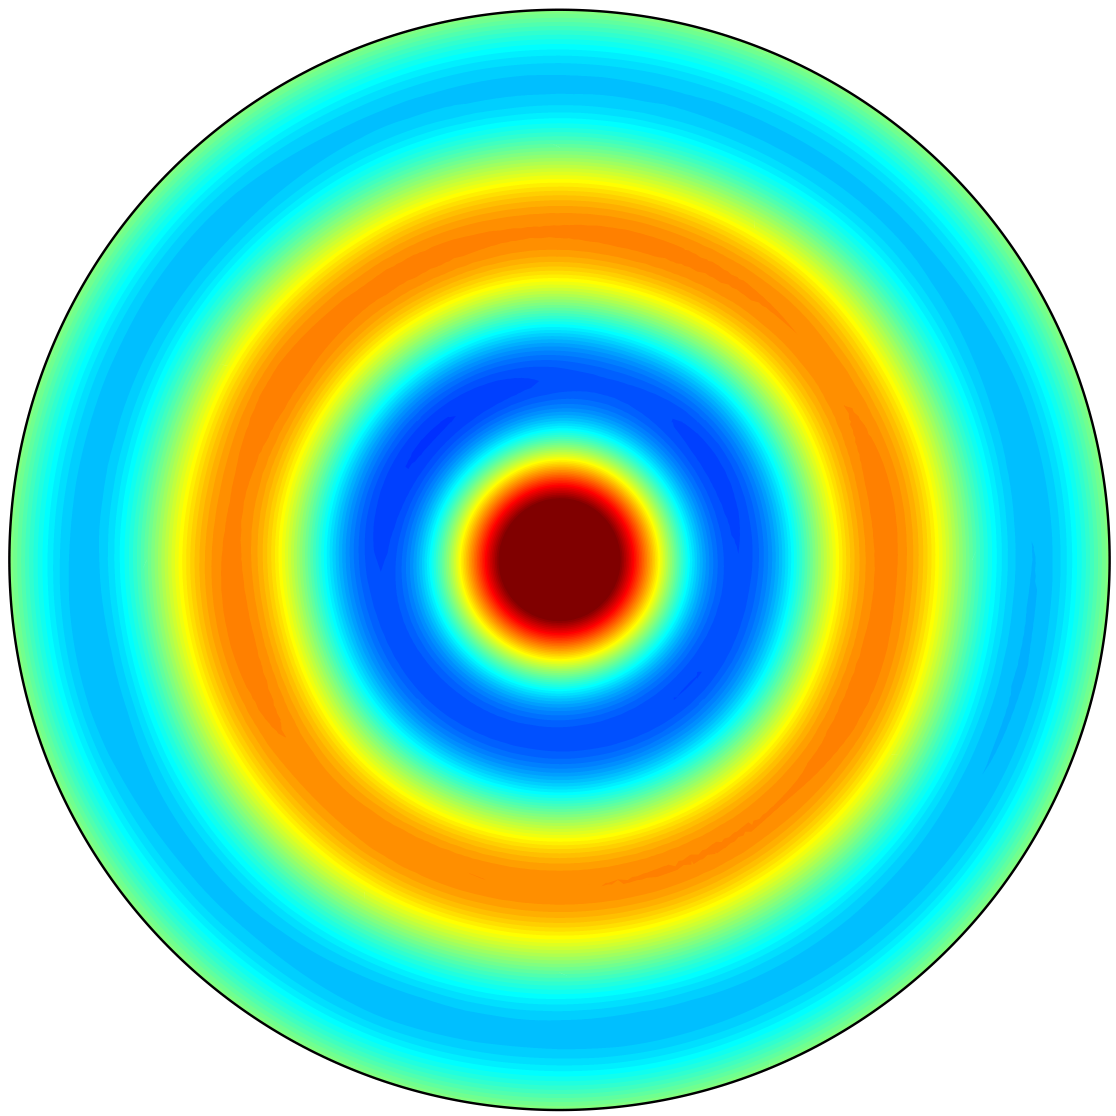
\includegraphics[width=0.24\textwidth] {2D_Circle/modeShapes/circleFreeSpace_mode17_U3}}
\subfigure[$f_{13} \approx$ 242.71 THz]{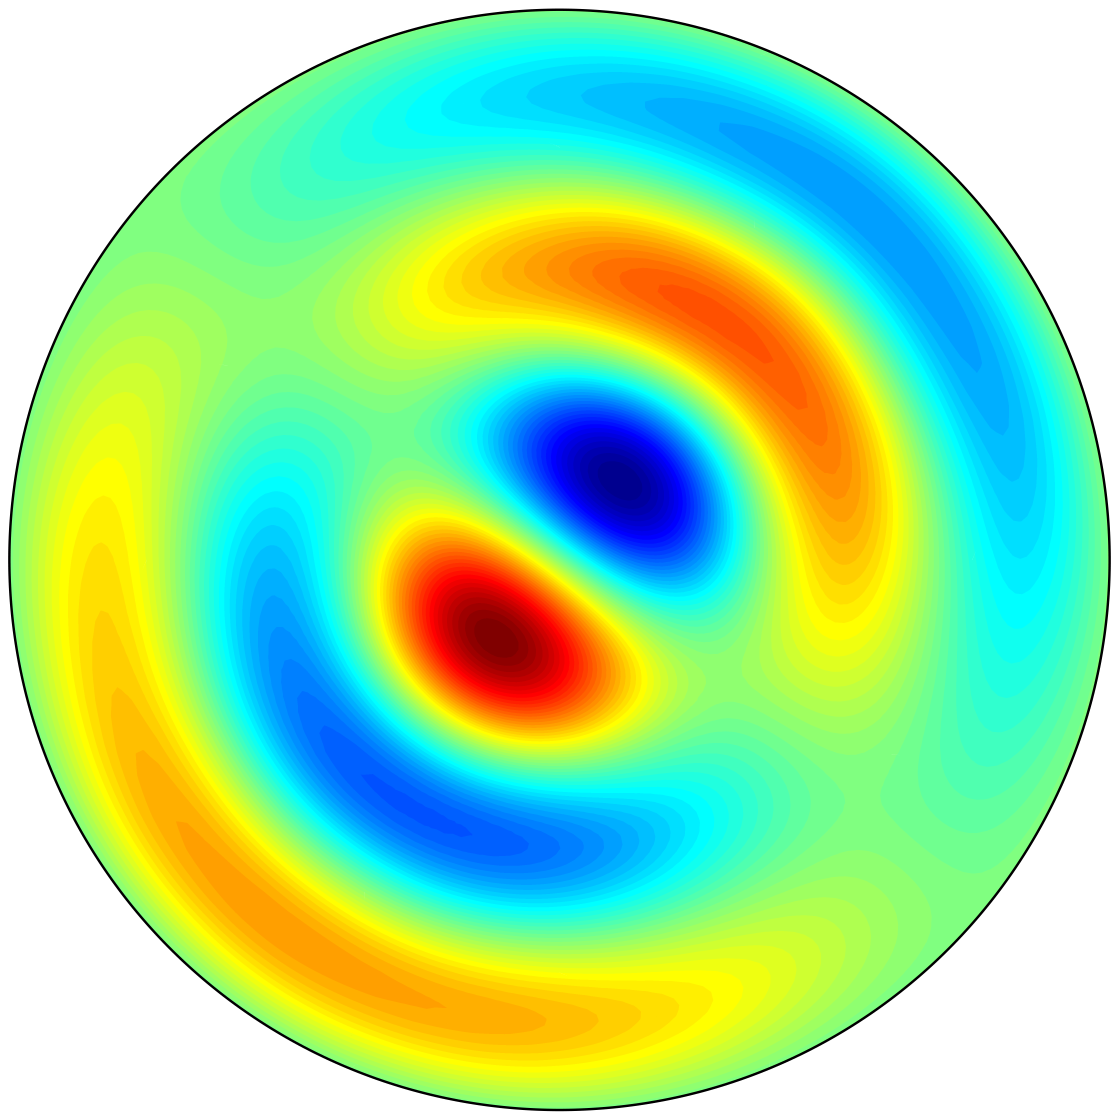
\includegraphics[width=0.24\textwidth] {2D_Circle/modeShapes/circleFreeSpace_mode13_U3}}
\subfigure[$f_7 \approx$ 181.03 THz]{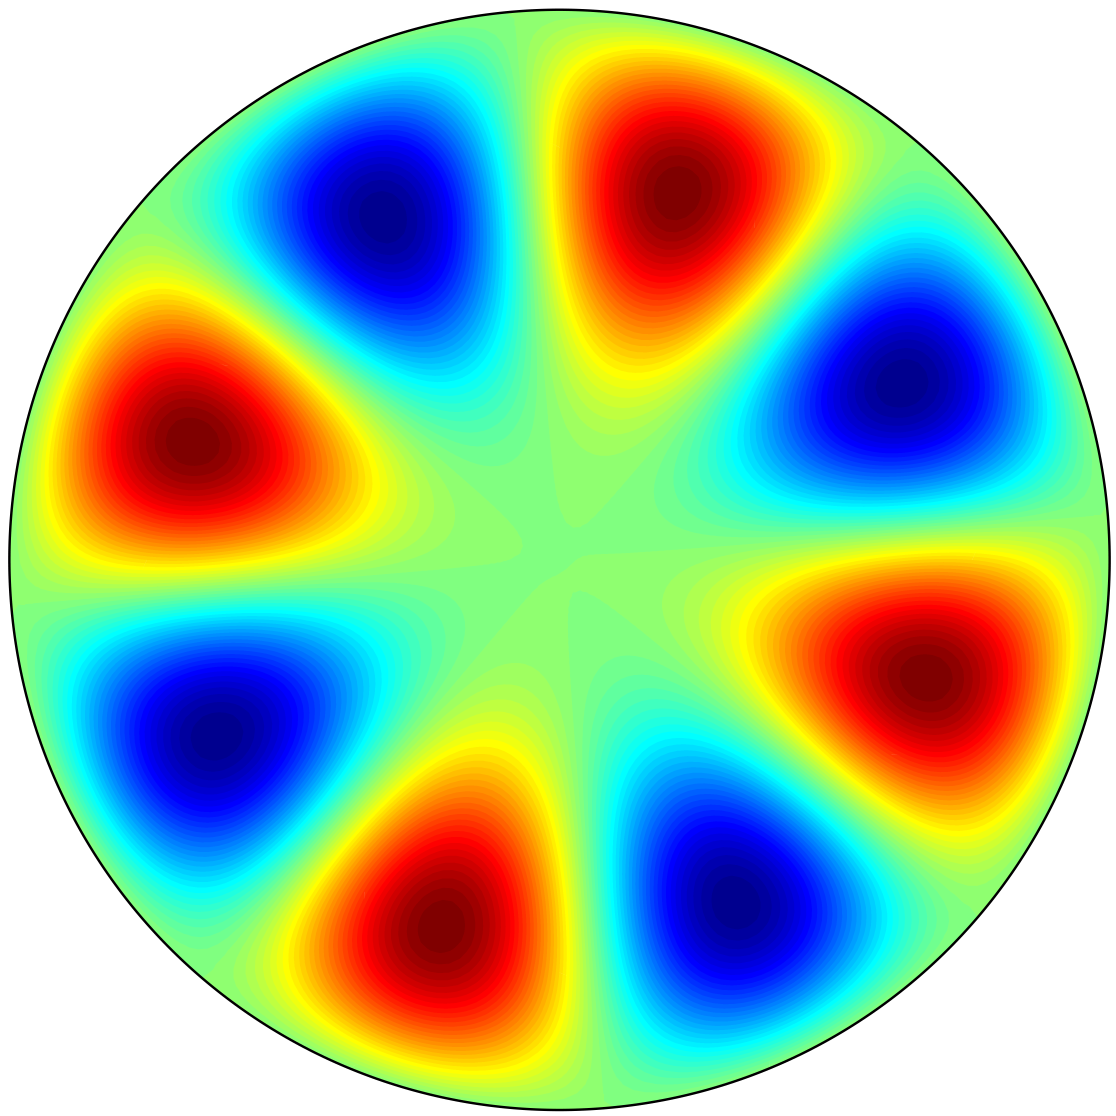
\includegraphics[width=0.24\textwidth] {2D_Circle/modeShapes/circleFreeSpace_mode7_U3}}
\subfigure[$f_{20} \approx$ 310.50 THz]{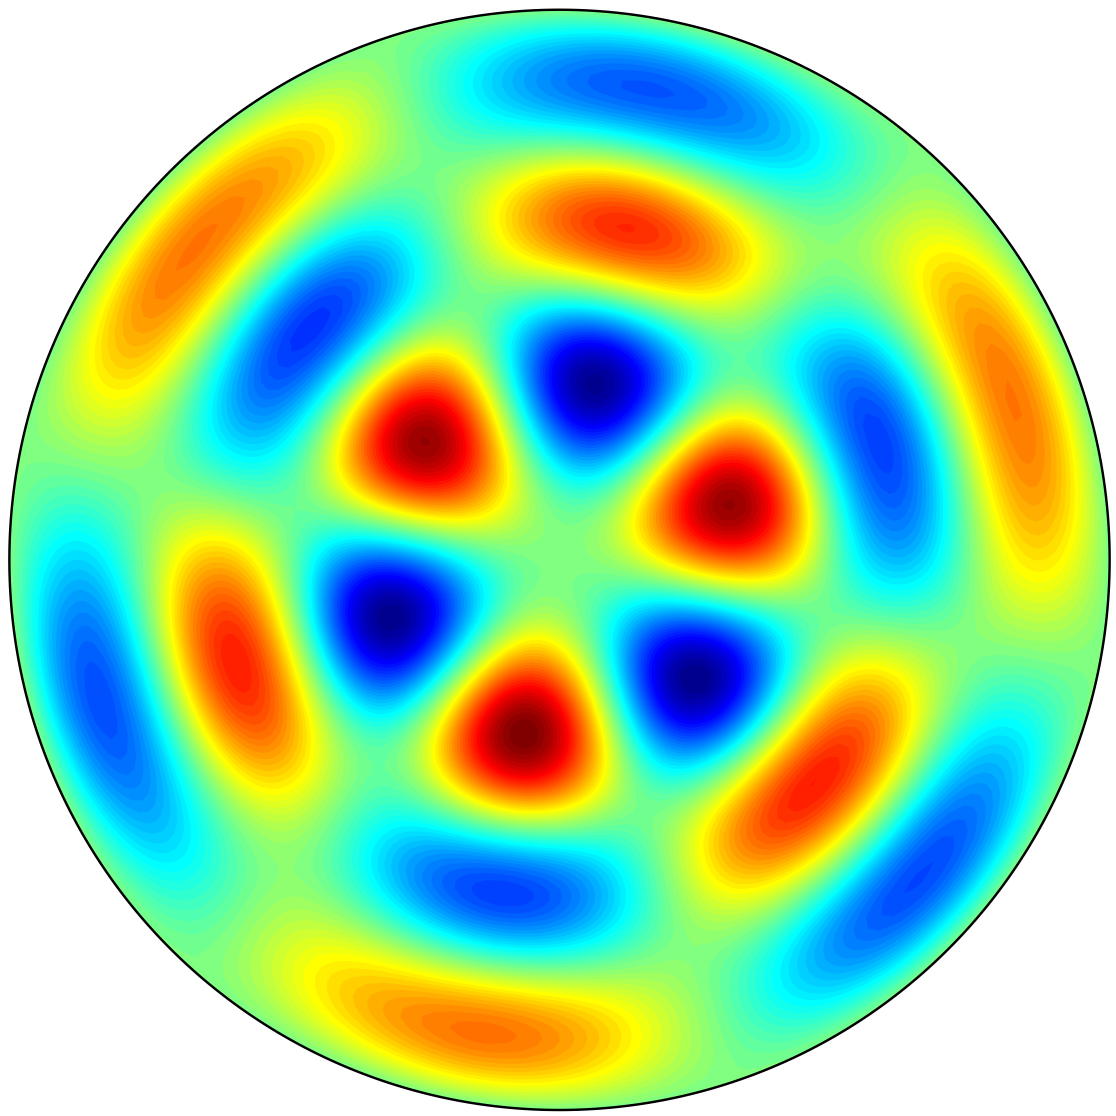
\includegraphics[width=0.24\textwidth] {2D_Circle/modeShapes/circleFreeSpace_mode20_U3}} 
\caption{Disk resonator: component $H_3$ of twelve resonant modes.}
\label{fig:circle2DfreeSpace_modes}
\end{figure}
%text
These modes are extracted by performing a discrete Fourier transform as described in Section~\ref{sc:FrequenciesAndModes}. All the modes were computed using a single time domain run on a mesh with 
only 1,024 elements and using a degree of approximation $p$=5 (i.e, 46,080 degrees of freedom) and the error on the highest computed resonant frequency ($f_{20} \approx$ 310.50 THz) is less than 0.3\%. This clearly illustrate the potential of the proposed approach for computing a broadband of resonant frequencies and the associated modes using NEFEM with a DG formulation in the time domain.

Next, the performance of both low and high-order approximations is studied. Figure~\ref{fig:circleHvsP} shows the evolution of the error of the first computed resonant frequency as a function of the number of degrees of freedom (\ndof) and the CPU time for low and high-order approximations. In both cases NEFEM is considered in order to avoid any error introduced by the polynomial approximation of curved boundaries inherent to standard isoparametric finite elements.
%figure REVISE : Circle convergence CPU times
\begin{figure}[!ht]
	\centering
	\subfigure[]{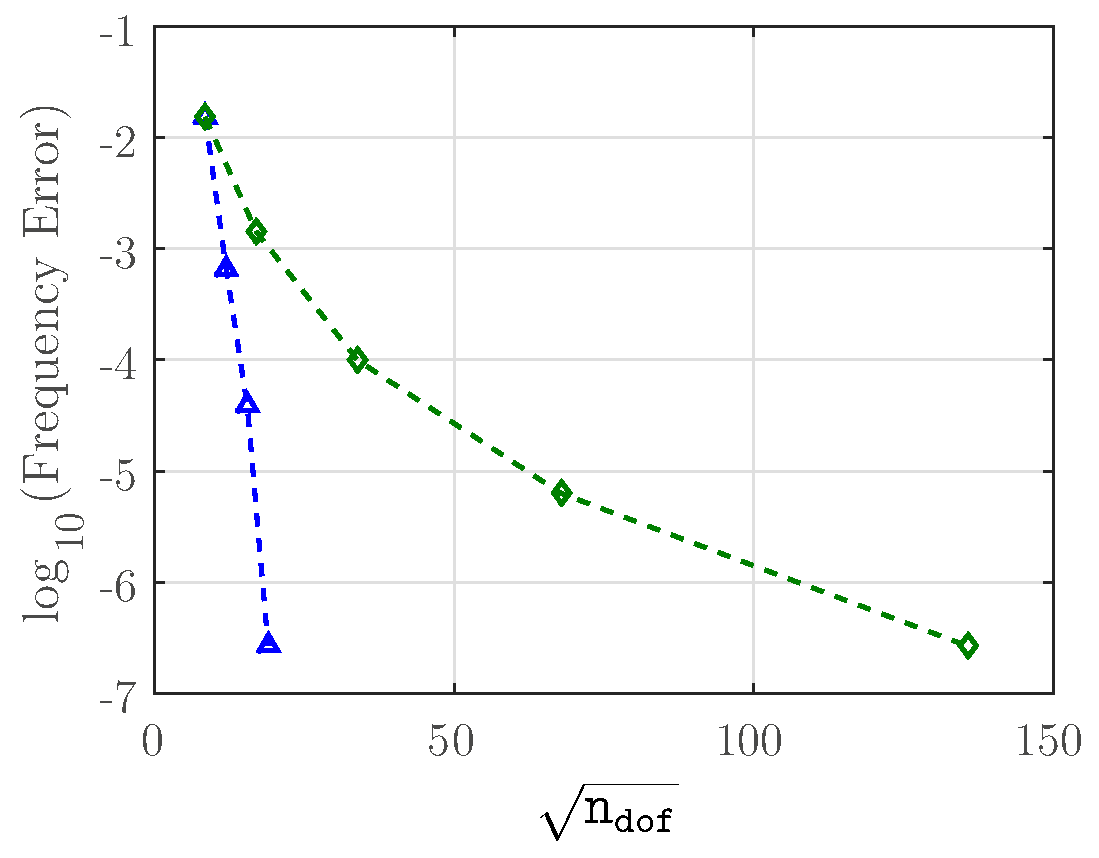
\includegraphics[width=0.49\textwidth]{figs/circleFreeSpace_ndof}}
	\subfigure[]{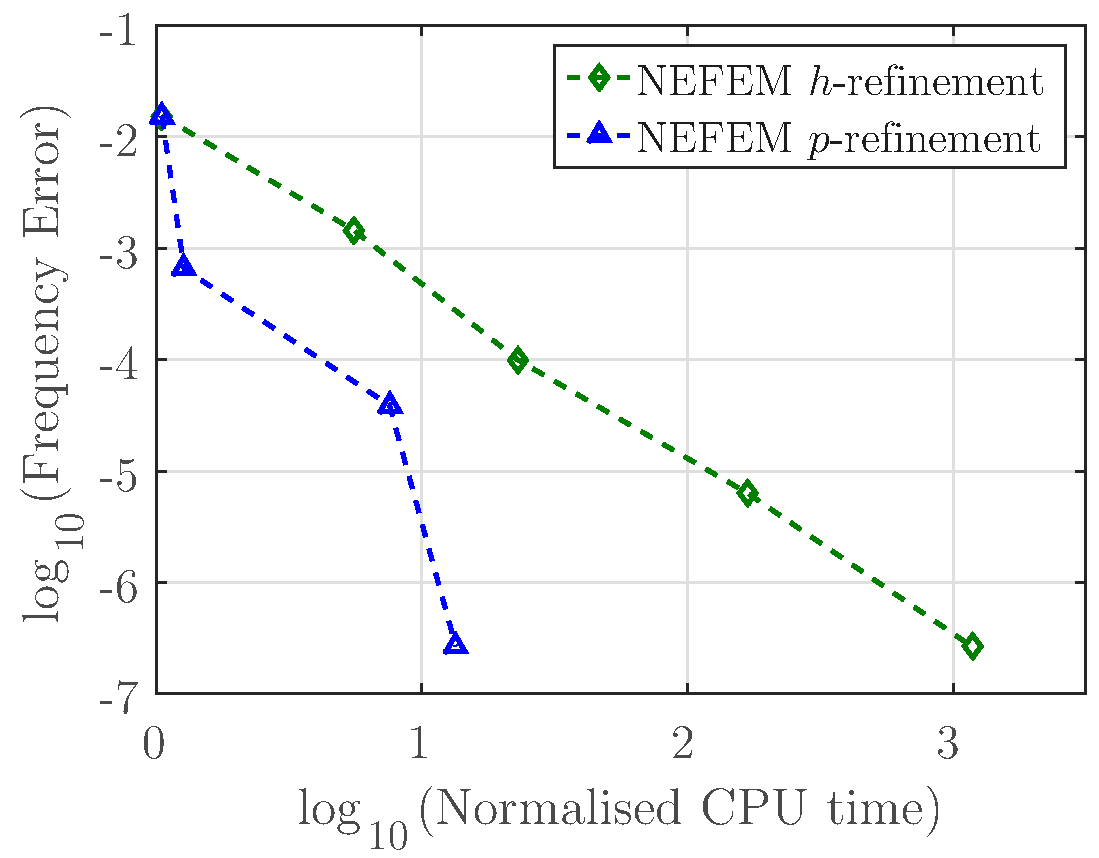
\includegraphics[width=0.49\textwidth]{figs/circleFreeSpace_cpu}}
	\caption{Disk resonator: Comparison of $h$ and $p$ refinement in terms of (a) the number of degrees of freedom (\ndof) and (b) the CPU time for the computation of the first resonant frequency $f_1 \approx$ 57.59 THz.}
	\label{fig:circleHvsP}
\end{figure}

%text
The comparison in terms of number of degrees of freedom in Figure~\ref{fig:circleHvsP} (a) shows, as expected that high-order elements significantly outperform low-order elements when the solution is smooth due to the exponential rate of convergence of a $p$-refinement strategy compared to the algebraic rate of an $h$-refinement strategy. In this example, for an error in the first resonant frequency of $10^{-4}$ the number of degrees of freedom required using NEFEM with linear approximation is 1,149, whereas the same accuracy can be obtained using approximately 204 degrees of freedom. For high accurate results, namely an error in the first resonant frequency of $2.5 \times 10^{-7}$, the use of high-order methods is even more advantageous. NEFEM with linear approximation requires 18,432 degrees of freedom, whereas the same accuracy can be obtained using only 360 degrees of freedom. 

The save in number of degrees of freedom introduced by a high-order functional approximation has been consistently observed in many examples and it is probably a crucial factor for the growing interest in high-order methods not only by the computational electromagnetics and but also by the computational fluid dynamics community~\cite{ADIGMA,HO-Fluids}. In some examples this save is not translated in a lower computational cost due to the extra computational cost per element induced by a high-order approximation. Figure~\ref{fig:circleHvsP} (b) shows the comparison of low and high-order approximations in terms of the normalised CPU time (i.e, dividing by the computational cost of linear elements in the coarse mesh) in logarithmic scale. The results demonstrate that high-order methods are not only competitive in terms of memory requirements, but more importantly, in terms of the computing time. In this example, an error in the first resonant frequency of $10^{-4}$ can be achieved using high-order elements 5.5 times faster than using linear elements. For high accurate results, namely an error in the first resonant frequency of $2.5 \times 10^{-7}$, high-order elements are 88 times faster than linear elements.

It is worth noting that the speed up factor of high-order elements compared to low-order elements is similar, or even higher, than the factor by which the number of degrees of freedom is reduced, clearly illustrating the potential and performance of high-order elements for the computation of resonant frequencies in cavities.


%============================================================
\clearpage
\subsection{Effect of the monitor position choice for cavities}
\clearpage
%figure TODO : Plots for effects of monitor positions - take them from ACME and change unit system as appropriate
\subsection{Rectangular dispersive cavity}
%text
The next example considers a rectangular cavity of dimension $2L \times L$, with $L=$20$\mu$m made of a dispersive material with non-dimensional constants $\omega_p = 0.7933$ and $\gamma = 0.076$ and with a perfect electric conducting boundary.

First, the implementation of the DG method for a lossless single-pole Drude media with no magnetic polarisation is validated by considering the propagation of a mode in the cavity. A volumetric source term is considered so that the analytical solution is
% 
\begin{equation*}
\E = \sin (\pi t) 
\begin{pmatrix}
- \cos (\pi x_1) \sin (\pi x_2) \\
  \sin (\pi x_1) \cos (\pi x_2) \\
2 \sin (\pi x_1) \sin (\pi x_2) 
\end{pmatrix}
%
\quad
%
\H = \cos (\pi t) 
\begin{pmatrix}
- \sin (\pi x_1) \cos (\pi x_2) \\
  \cos (\pi x_1) \sin (\pi x_2) \\
- \cos (\pi x_1) \cos (\pi x_2) 
\end{pmatrix}.
\end{equation*}

The computations are performed on a series of structured quadrilateral meshes with 4$\times$2, 8$\times$4, 16$\times$8, 32$\times$16,  64$\times$32 and 128$\times$64 elements and for a degree of approximation from $p$=1 to $p$=4. Initial and boundary conditions corresponding to the analytical solution are considered.

Figure~\ref{fig:rectangle2DdispersiveTest_Convergence} shows the $\mathcal{L}^2(\Omega)$ norm of the error of two components of the electromagnetic field, namely $E_1$ and $H_3$, as a function of the characteristic element size $h$. In all cases, the expected optimal rate of convergence (i.e, $p$+1) is observed. 
%figure DONE: Volumetric source convergence
\begin{figure}[!ht]
	\centering
	\subfigure[$E_1$]{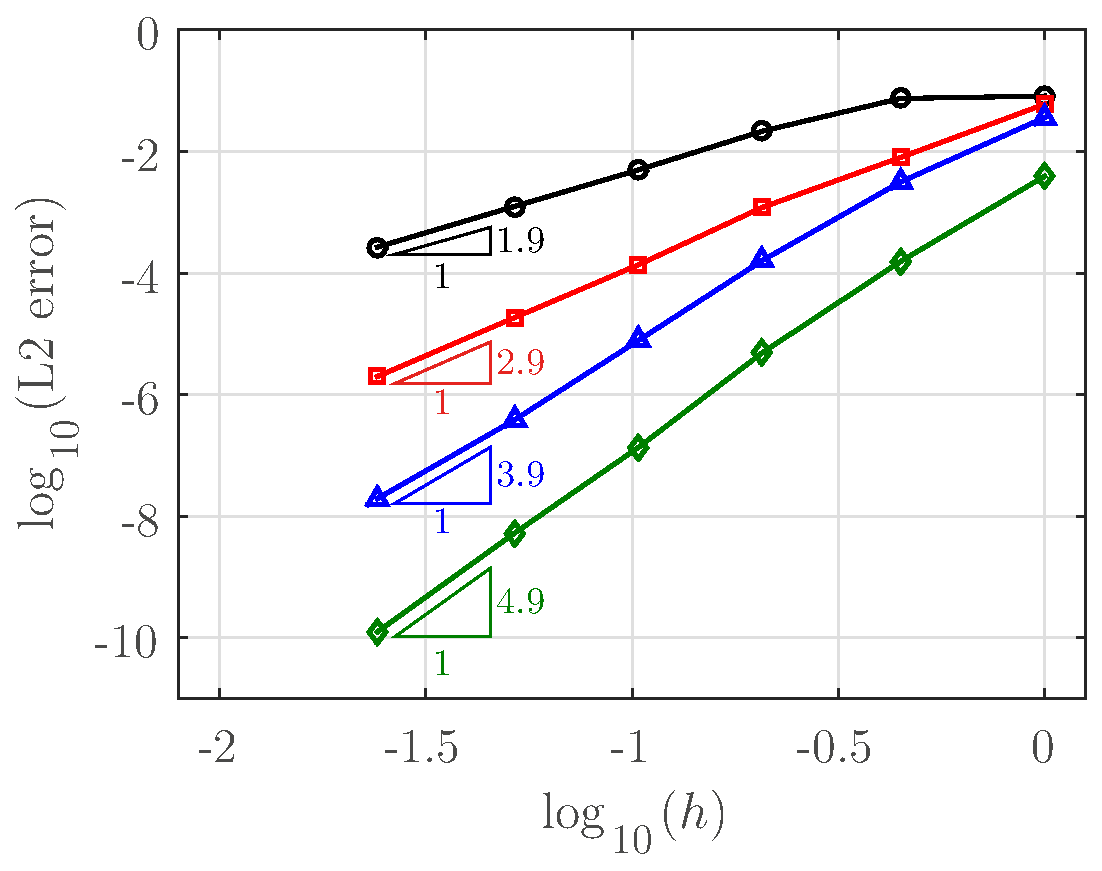
\includegraphics[width=0.49\textwidth]{figs/dispersiveHconv_U1}}
	\subfigure[$H_3$]{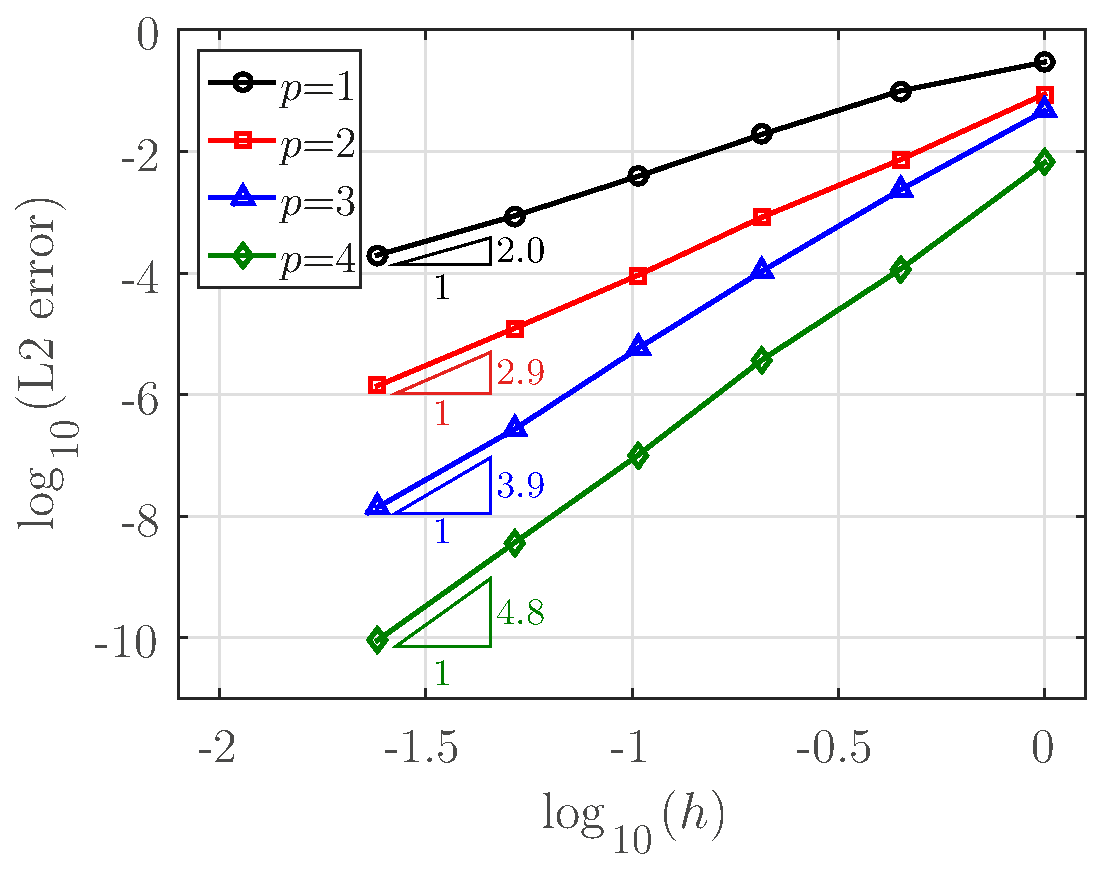
\includegraphics[width=0.49\textwidth]{figs/dispersiveHconv_U3}}
	\caption{Rectangular dispersive cavity: $h$-convergence of the $\mathcal{L}^2(\Omega)$ norm of the error of two components of the electromagnetic field as a function of the characteristic element size $h$ for different degrees of approximation ($p$).}
	\label{fig:rectangle2DdispersiveTest_Convergence}
\end{figure}
%text
Next, the convergence properties of the proposed technique for the computation of resonant frequencies in a dispersive cavity are validated. As no analytical solution is available for the resonant frequencies, a reference solution is computed using a mesh with 2048 elements and a degree of approximation $p$=3.  The error in the computed frequency $f_i$ is evaluated as $\epsilon_i = (|f_i - f_i^r|)/f_i^r$, where $f_i^r$ is the reference value of the resonant frequency.

Figure~\ref{fig:rectangle2Ddispersive_Convergence} shows the evolution of the error on two computed resonant frequencies as a function of the element size for linear and quadratic elements. 
%figure DONE: dispersive convergence
\begin{figure}[!ht]
	\centering

\subfigure[$f_{3},\USoltn_{3} $]{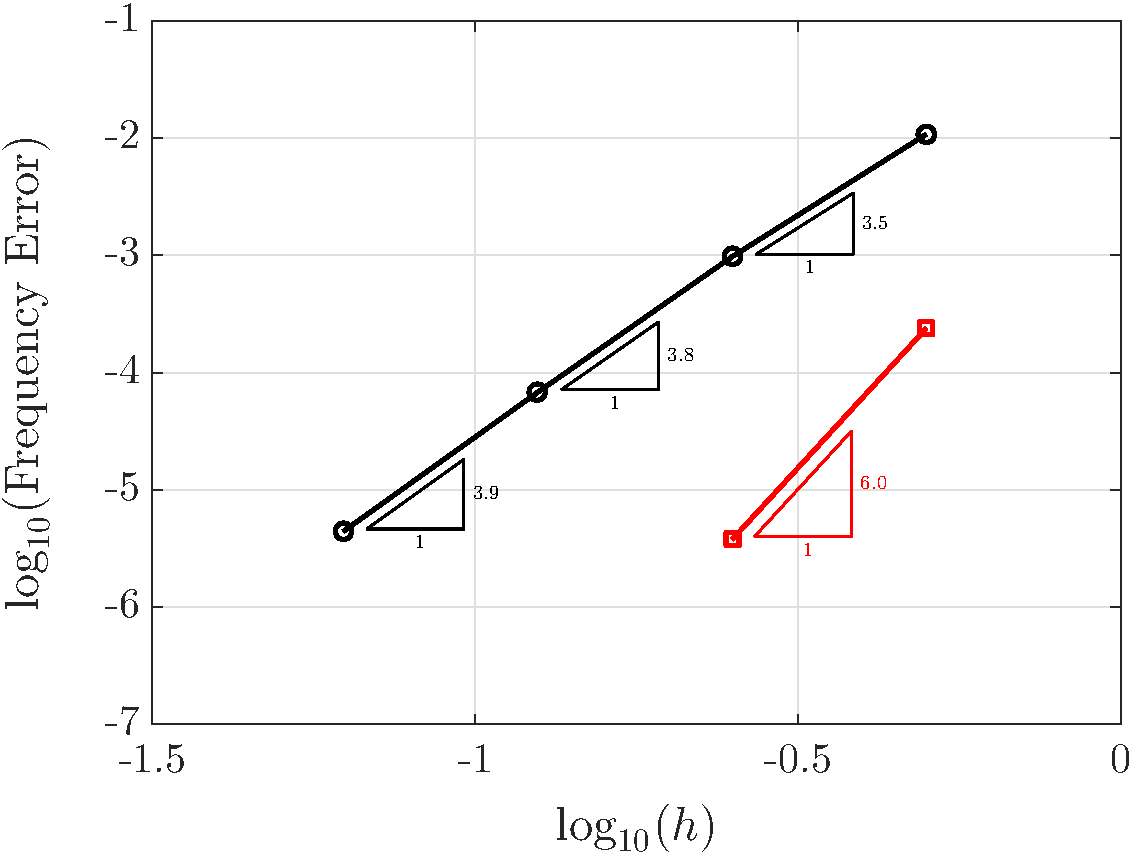
\includegraphics[width=0.49\textwidth]{2D_DispersivePlate/Conv/F3_U3_TM}}
\subfigure[$f_{6},\USoltn_{3} $]{\includegraphics[width=0.49\textwidth]{2D_DispersivePlate/Conv/F6_U3_TM}}
\subfigure[$f_{8},\USoltn_{3} $]{\includegraphics[width=0.49\textwidth]{2D_DispersivePlate/Conv/F8_U3_TM}}
\subfigure[$f_{9},\USoltn_{2} $]{\includegraphics[width=0.49\textwidth]{2D_DispersivePlate/Conv/F9_U2_TM}}
\subfigure[$f_{10},\USoltn_{3} $]{\includegraphics[width=0.49\textwidth]{2D_DispersivePlate/Conv/F10_U3_TM} }
	\caption{Rectangular dispersive cavity: $h$-convergence of the error for two resonant frequencies.}
	\label{fig:rectangle2Ddispersive_Convergence}
\end{figure}
%text
In all the examples, the expected $2p+2$ rate of convergence is approximately obtained, confirming the optimality of the proposed approach for computing the resonant frequencies of cavities filled with dispersive materials. As in previous examples, it can be observed that, for a given mesh and degree of approximation, the error increases as the frequency increases, illustrating the challenge in approximating higher frequencies. 


The effect of the dispersive material in the signal recorded at a point of the cavity is shown in Figure~\ref{fig:freeSpaceDispersiveSignal} by comparing the results to the ones obtained in the free-space cavity discussed in Section~\ref{sbc:freeSpace2D}.
%figure DONE: dispersive signal(unfiltered)
\begin{figure}[!ht]
	\centering
	\subfigure[]{\includegraphics[width=0.49\textwidth]{figs/freeSpaceDispersiveSignal1}}
	\subfigure[]{\includegraphics[width=0.49\textwidth]{figs/freeSpaceDispersiveSignal2}}
	\caption{Rectangular dispersive cavity: Comparison of the time recorded signal corresponding to the component $H_3$ at a point of the cavity for free-space and dispersive media.}
	\label{fig:freeSpaceDispersiveSignal}
\end{figure}
%text
It can be observed in Figure~\ref{fig:freeSpaceDispersiveSignal}(a) that in initially the signals are very similar in shape and phase despite important differences are already observed in the amplitude. As represented in Figure~\ref{fig:freeSpaceDispersiveSignal}(b) for latter times the recorded signals vary significantly.

Finally, Figure~\ref{fig:dispersiveFreeSpaceSpectrum} shows the computed spectrum for both the free-space cavity and the dispersive cavity using, in both cases, a mesh with 128 elements and a degree of approximation $p$=2. 
%figure LATER: dispersive spectrum comparison -  can I do better?
\begin{figure}[!ht]
\centering
\includegraphics[width=0.6\textwidth]{figs/dispersiveFreeSpaceSpectrum}
\caption{Rectangular dispersive cavity: Comparison of computed spectra for a for free-space and dispersive cavity.}
\label{fig:dispersiveFreeSpaceSpectrum}
\end{figure}
%text
The results reveal a shift of all the frequencies, being more important for low frequencies than for the higher frequencies. It can also be observed that the amplitude is lower for the dispersive cavity compared to the cavity filled with air.


%============================================================
\clearpage
\subsection{Three dimensional cavities with planar faces}
%text
The next example considers a three dimensional metallic cavity of dimension $L\times L \times L$, where $L$=2$\mu$m filled with air, for which an analytical solution is known~\cite{BalanisBook}. The objective is to validate the implementation and illustrate the potential of the proposed approach in three dimensions.  

The frequencies are computed using a series of structured hexahedral meshes with 2$\times$2$\times$2, 4$\times$4$\times$4, 8$\times$8$\times$8 and 16$\times$16$\times$16 elements and different degrees of approximation. Although the use of tetrahedral meshes is preferred for geometrically complex cavities, the use of hexahedral elements, when possible, reduces significantly the cost of the time domain solver due to the reduced number of interior faces compared to a tetrahedral mesh. The performance of different elements was studied in detail in~\cite{HybridMeshesCEM} and it was concluded that in order to obtain the same accuracy hexahedral elements require between 10 to 15 less computational time than tetrahedral elements.

The evolution of the error on two computed resonant frequencies as a function of the element size for a degree of approximation $p$ ranging from 1 up to 3 is shown in Figure~\ref{fig:cube3DfreeSpace_ConvergenceTet} for tetrahedral elements and in Figure~\ref{fig:cube3DfreeSpace_ConvergenceHex} for hexahedral elements.

\begin{figure}[!ht]
	\centering
	\subfigure[$f_5    \approx$ 1.118, $\USoltn_{1}$]{\includegraphics[width=0.49\textwidth]{3D_CubeCavity/Conv/HEX/U[1]/F5_CF}}
	\subfigure[$f_6    \approx$ 1.225, $\USoltn_{6}$]{\includegraphics[width=0.49\textwidth]{3D_CubeCavity/Conv/HEX/U[6]/F6_CF}}
	\subfigure[$f_9    \approx$ 1.581, $\USoltn_{4}$]{\includegraphics[width=0.49\textwidth]{3D_CubeCavity/Conv/HEX/U[4]/F9_CF}}
	\subfigure[$f_{10} \approx$ 1.658, $\USoltn_{2}$]{\includegraphics[width=0.49\textwidth]{3D_CubeCavity/Conv/HEX/U[2]/F10_CF}}

	\caption{Three dimensional cavity: $h$-convergence of the error for a selection of four choices of resonant frequency and solution component using hexahedral elements.}
	\label{fig:cube3DfreeSpace_ConvergenceHex}
\end{figure}

\begin{figure}[!ht]
	\centering
	\subfigure[$f_5    \approx$ 1.118, $\USoltn_{3}$]{\includegraphics[width=0.49\textwidth]{3D_CubeCavity/Conv/TET/U[1]/F5_CF}}
	\subfigure[$f_6    \approx$ 1.225, $\USoltn_{6}$]{\includegraphics[width=0.49\textwidth]{3D_CubeCavity/Conv/TET/U[6]/F6_CF}}
	\subfigure[$f_9    \approx$ 1.581, $\USoltn_{4}$]{\includegraphics[width=0.49\textwidth]{3D_CubeCavity/Conv/TET/U[4]/F9_CF}}
	\subfigure[$f_{10} \approx$ 1.658, $\USoltn_{2}$]{\includegraphics[width=0.49\textwidth]{3D_CubeCavity/Conv/TET/U[2]/F10_CF}}

	\caption{Three dimensional cavity: $h$-convergence of the error for a selection of four choices of resonant frequency and solution component using tetrahedral elements.}
	\label{fig:cube3DfreeSpace_ConvergenceTet}
\end{figure}
%text
The results demonstrate the optimal convergence properties of the proposed approach to compute the resonant frequencies in three dimensional cavities and illustrate the challenge of computing high resonant frequencies as the accuracy of the frequency $f_5$ is almost two orders of magnitude higher than the accuracy for the frequency $f_9$. 

In addition, it is important to remark that the save in terms of number of degrees of freedom is more significant here than for the two dimensional problems discussed before. For instance, in order to obtain a relative error on the frequency $f_9$ below $10^{-4}$, cubic elements employ a mesh with 64 elements (i.e, 1,280 degrees of freedom), quadratic elements require a mesh with 512 elements (i.e, 5,120 degrees of freedom) and linear elements require a further level of mesh refinement (not considered in Figure~\ref{fig:cube3DfreeSpace_Convergence}(b)), resulting in a mesh with 32,768 elements (i.e, 131,072 degrees of freedom). This means that cubic elements are able to perform a similar accuracy compared to linear elements by reducing the number of degrees of freedom by more than two orders of magnitude.

The resonant modes are again computed using another time domain simulation as described in Section~\ref{sc:FrequenciesAndModes}. Figure~\ref{fig:cubeFreeSpace_1stMode} shows the three components of the electric field for the resonant mode associated to the lowest frequency, $f_1 \approx$ 105.99 THz.
%figure DONE: 3D Cube mode shapes different components
\begin{figure}[!ht]
	\centering
	\subfigure[$E_1$]{\includegraphics[width=0.32\textwidth] {3D_CubeCavity/modeShapes/Cube_Mode2_U1}}
	\subfigure[$E_2$]{\includegraphics[width=0.32\textwidth] {3D_CubeCavity/modeShapes/Cube_Mode2_U2}}
	\subfigure[$E_3$]{\includegraphics[width=0.32\textwidth] {3D_CubeCavity/modeShapes/Cube_Mode2_U3}}
	\caption{Three dimensional cavity: three components of the electric field for the first resonant mode with frequency $f_1 \approx$ 105.99 THz.}
	\label{fig:cubeFreeSpace_1stMode}
\end{figure}

%text
To further illustrate the potential of the proposed methodology, Figure~\ref{fig:cubeFreeSpace_modes} shows the intensity of the electric and magnetic fields for four resonant modes, associated to the resonant frequencies $f_4\approx$ 167.59 THz, $f_6\!\approx$ 211.99 THz, $f_{35} \approx$ 491.47 THz and $f_{36} \approx$ 502.77 THz.
%figure TODO: better 3D Cube mode shapes
\begin{figure}[!ht]
	\centering
	\subfigure[$\!\!\!E, f_4\!\approx$167.6 THz]{\includegraphics[width=0.24\textwidth]{3D_CubeCavity/modeShapes/Cube_Mode5_E}}
	\subfigure[$\!\!\!E, f_6\!\approx$212.0 THz]{\includegraphics[width=0.24\textwidth]{3D_CubeCavity/modeShapes/Cube_Mode7_E}}
	\subfigure[$\!\!\!E, f_{35}\!\approx$491.5 THz]{\includegraphics[width=0.24\textwidth]{3D_CubeCavity/modeShapes/Cube_Mode36_E}}
	\subfigure[$\!\!\!E, f_{36}\!\approx$502.8 THz]{\includegraphics[width=0.24\textwidth]{3D_CubeCavity/modeShapes/Cube_Mode37_E}} \\
	\subfigure[$\!\!\!H, f_4\!\approx$167.6 THz]{\includegraphics[width=0.24\textwidth]{3D_CubeCavity/modeShapes/Cube_Mode5_H}}
	\subfigure[$\!\!\!H, f_6\!\approx$212.0 THz]{\includegraphics[width=0.24\textwidth]{3D_CubeCavity/modeShapes/Cube_Mode7_H}}
	\subfigure[$\!\!\!H, f_{35}\!\approx$491.5 THz]{\includegraphics[width=0.24\textwidth]{3D_CubeCavity/modeShapes/Cube_Mode36_H}}
	\subfigure[$\!\!\!H, f_{36}\!\approx$502.8 THz]{\includegraphics[width=0.24\textwidth]{3D_CubeCavity/modeShapes/Cube_Mode37_H}} 
	\caption{Three dimensional cavity: intensity of the electric (top) and magnetic (bottom) fields for four resonant modes.}
	\label{fig:cubeFreeSpace_modes}
\end{figure}

%text
All the modes have been computed on a mesh with only 64 hexahedral elements and using a degree of approximation $p=3$ (i.e, 7,680 degrees of freedom) and the relative error in the four resonant frequencies associated to the mode represented in Figure~\ref{fig:cubeFreeSpace_modes}, ranging from 167.59 THz to 502.77 THz is below $10^{-5}$.

\clearpage
\subsection{Three dimensional cavities with curved faces}
%text TODO introduce 3D Sphere
%figures TODO show some figures of 3D Sphere

\clearpage
\subsection{Cavities with small features}
%figure
\begin{figure}[!ht]
	\centering
\subfigure[without scatterers]{\includegraphics[width=0.49\textwidth]{NotchedAndSpiral/peakCircleOnly}}
\subfigure[with scatterers]{\includegraphics[width=0.49\textwidth]{NotchedAndSpiral/peakNotchOnly}}
\subfigure[with and without scatterers]{\includegraphics[width=0.49\textwidth]{NotchedAndSpiral/peakNotchAndCircle}}
	\caption{Rectangular dispersive cavity: $h$-convergence of the error for two resonant frequencies.}
	\label{fig:rectangle2Ddispersive_Convergence}
\end{figure}
%text TODO introduce 3D Sphere
\section{Parallel}
\subsection{3D Convergence plots}
\begin{figure}[!ht]
	\centering
  \includegraphics[width=0.49\textwidth]{Parallel/3DSpeedPlot_unitCube_legend}
	\caption{3D unit cube: timings obtained with a non-uniform mesh}
	\label{fig:unitCubeNonUniformTimings}
\end{figure}
\clearpage
\subsection{3D Non-Uniform Cube}
speed(normalised): 0.5551    0.6592    1.0000
(computed from minimum timestep length)
\begin{figure}[!ht]
	\centering
  \subfigure[unweighted]{\includegraphics[width=0.49\textwidth]{Parallel/3D_UnitCube_nonUniform/noWeighting}} \\
  \subfigure[by measurement]{\includegraphics[width=0.49\textwidth]{Parallel/3D_UnitCube_nonUniform/computedWeighting}}
  \subfigure[by operation count]{\includegraphics[width=0.49\textwidth]{Parallel/3D_UnitCube_nonUniform/analyticalWeighting}}
	\caption{3D unit cube: timings obtained with a non-uniform mesh}
	\label{fig:unitCubeNonUniformTimings}
\end{figure}

16689 elements
3437 nodes
Tets
\begin{figure}[!ht]
	\centering
\subfigure[]{\includegraphics[width=0.49\textwidth]{Parallel/3D_UnitCube_nonUniform/weightingComparison_legend}}
\caption{3D unit cube: weighting comparison}
	\label{fig:unitCubeNonUniformTimings}
\end{figure}
\begin{figure}[!ht]
	\centering
  \subfigure[histogram]{\includegraphics[width=0.49\textwidth]{Parallel/3D_UnitCube_nonUniform/elementSizeHsitogram}}
  \subfigure[histogram]{\includegraphics[width=0.49\textwidth]{Parallel/3D_UnitCube_nonUniform/pHistogram}}
\caption{3D unit cube: histograms of p and element size}
	\label{fig:unitCubeNonUniformTimings}
\end{figure}

change in delta t is only 6x
hMin=0.003963734230961


\section{Variable order}
%figure done 3D Cube Exploded
\begin{figure}[!ht]
	\centering
  \includegraphics[width=\textwidth]{3D_SphereExploded/sphereDots}
	\caption{3D unit cube: timings obtained with a non-uniform mesh}
	\label{fig:unitCubeNonUniformAdaptiveP}
\end{figure}
\begin{figure}[!ht]
	\centering
\includegraphics[width=\textwidth]{Parallel/globalL2Convergence}
\caption{3D unit cube: global convergence of L2 norm of the solution}
	\label{fig:unitCubeNonUniformGlobalAdaptivePL2Conv}
\end{figure}
L2 computed at $T=1$
\begin{figure}[!ht]
	\centering
\subfigure[]{\includegraphics[width=0.49\textwidth]{/home/mark/Data/ForHardDrive/AdaptiveP/local_convergence/localConvergenceFrame0_legend}}
\subfigure[]{\includegraphics[width=0.49\textwidth]{/home/mark/Data/ForHardDrive/AdaptiveP/local_convergence/localConvergenceFrame1}}
\end{figure}
\begin{figure}[!ht]
	\centering
  \includegraphics[width=\textwidth]{pAdaptivity/localConvergence/nestedElementsWithoutP}
\caption{3D unit cube: histograms of p and element size}
	\label{fig:unitCubeNonUniformTimings}
\end{figure}
% text TODO
%% * use the same dimensions as the 3D Cube
\section{Photonic Crystals}
\begin{figure}[!ht]
	\centering
  \includegraphics[width=0.49\textwidth]{PhC/PhCHexagonal}
\end{figure}
NEFEM mesh
TODO: mesh details (number of elements etc)
\begin{figure}[!ht]
	\centering
\subfigure[$f_{2}, \USoltn_{3}$]{\includegraphics[width=0.49\textwidth]{PhC/modeShapes/frame2_U3_nurbsZoom}}
\subfigure[$f_{5}, \USoltn_{2}$]{\includegraphics[width=0.49\textwidth]{PhC/modeShapes/frame5_U2_nurbsZoom}}
\subfigure[$f_{4}, \USoltn_{2}$]{\includegraphics[width=0.49\textwidth]{PhC/modeShapes/frame4_U2_nurbsZoom}}
\subfigure[$f_{3}, \USoltn_{3}$]{\includegraphics[width=0.49\textwidth]{PhC/modeShapes/frame3_U3_nurbsZoom}}
\subfigure[$f_{1}, \USoltn_{3}$]{\includegraphics[width=0.49\textwidth]{PhC/modeShapes/frame1_U3_nurbsZoom}}
\subfigure[$f_{7}, \USoltn_{1}$]{\includegraphics[width=0.49\textwidth]{PhC/modeShapes/frame7_U1_nurbsZoom}}
\subfigure[$f_{5}, \USoltn_{3}$]{\includegraphics[width=0.49\textwidth]{PhC/modeShapes/frame5_U3_nurbsZoom}}
\subfigure[$f_{7}, \USoltn_{3}$]{\includegraphics[width=0.49\textwidth]{PhC/modeShapes/frame7_U3_nurbsZoom}}
\subfigure[$f_{3}, \USoltn_{2}$]{\includegraphics[width=0.49\textwidth]{PhC/modeShapes/frame3_U2_nurbsZoom}}
\subfigure[$f_{1}, \USoltn_{2}$]{\includegraphics[width=0.49\textwidth]{PhC/modeShapes/frame1_U2_nurbsZoom}}
\subfigure[$f_{3}, \USoltn_{1}$]{\includegraphics[width=0.49\textwidth]{PhC/modeShapes/frame3_U1_nurbsZoom}}
\subfigure[$f_{1}, \USoltn_{1}$]{\includegraphics[width=0.49\textwidth]{PhC/modeShapes/frame1_U1_nurbsZoom}}
\subfigure[$f_{7}, \USoltn_{2}$]{\includegraphics[width=0.49\textwidth]{PhC/modeShapes/frame7_U2_nurbsZoom}}
\subfigure[$f_{9}, \USoltn_{3}$]{\includegraphics[width=0.49\textwidth]{PhC/modeShapes/frame9_U3_nurbsZoom}}
\subfigure[$f_{4}, \USoltn_{1}$]{\includegraphics[width=0.49\textwidth]{Figures/PhC/modeShapes/frame4_U1_nurbsZoom}}
\end{figure}

\section{3D Computations}
% TODO : remember the stuff I did for the more accurate timestepping...! 
%text ENDDOC
%%% Local Variables:
%%% mode: latex
%%% TeX-master: "../Thesis"
%%% End:
